\documentclass[notheorems,compress,mathserif,table]{beamer}

\useoutertheme{tree}
\usecolortheme{whale}      % Outer color themes, 其他选择: whale, seahorse, dolphin . 换一个编译看看有什么不同.
\usecolortheme{orchid}     % Inner color themes, 其他选择: lily, orchid
\useinnertheme[shadow]{rounded} % 对 box 的设置: 圆角、有阴影.
\setbeamercolor{sidebar}{bg=blue!50} % sidebar的颜色, 50%的蓝色.
%\setbeamercolor{background canvas}{bg=blue!9} % 背景色, 9%的蓝色. 去掉下一行, 试一试这个.
\setbeamertemplate{background canvas}[vertical shading][bottom=white,top=structure.fg!25] %%背景色, 上25%的蓝, 过渡到下白.
\usefonttheme{serif}  % 字体. 个人偏好有轮廓的字体. 去掉这个设置编译, 就看到不同了.
\setbeamertemplate{navigation symbols}{}   %% 去掉页面下方默认的导航条.
%%------------------------常用宏包---------------------------------------------------------------------
%%注意, beamer 会默认使用下列宏包: amsthm, graphicx, hyperref, color, xcolor, 等等
%\usepackage{CJK}
\usepackage{ctex}
\usepackage{amsmath,amsthm,amsfonts,amssymb,bm}
\usepackage{mathrsfs}
\usepackage{subfigure} %%图形或表格并排排列
\usepackage{xmpmulti}  %%支持文中的 \multiinclude 等命令, 使 mp 文件逐帧出现. 具体讨论见 beamer 手册.
\usepackage{colortbl,dcolumn}     %% 彩色表格
%\logo{
\includegraphics[height=0.09\textwidth]{ajln.jpg}}   %左上角科大logo
%%%%%%%%%%%%%%%%%%%%%%%%%%%%%%%%%%%%%%重定义字体、字号命令 %%%%%%%%%%%%%%%%%%%%%%%%%%%%%%%%%%%%%%%%%%%%%%
%\newcommand{\songti}{\CJKfamily{song}}        % 宋体
%\newcommand{\fangsong}{\CJKfamily{fs}}        % 仿宋体
%\newcommand{\kaishu}{\CJKfamily{kai}}         % 楷体
%\newcommand{\heiti}{\CJKfamily{hei}}          % 黑体
%\newcommand{\lishu}{\CJKfamily{li}}           % 隶书
\newcommand{\youyuang}{\CJKfamily{you}}       % 幼圆
\newcommand{\sanhao}{\fontsize{16pt}{\baselineskip}\selectfont}     % 字号设置
\newcommand{\sihao}{\fontsize{14pt}{\baselineskip}\selectfont}      % 字号设置
\newcommand{\xiaosihao}{\fontsize{12pt}{\baselineskip}\selectfont}  % 字号设置
\newcommand{\wuhao}{\fontsize{10.5pt}{\baselineskip}\selectfont}    % 字号设置
\newcommand{\xiaowuhao}{\fontsize{9pt}{\baselineskip}\selectfont}   % 字号设置
\newcommand{\liuhao}{\fontsize{7.875pt}{\baselineskip}\selectfont}  % 字号设置
\newcommand{\qihao}{\fontsize{5.25pt}{\baselineskip}\selectfont}    % 字号设置
%%%%%%%%%%%%%%%%%%%%%%%%%%%%%%%%%%%%%%%%%%%%%%%%%%%%%%%%%%%%%%%%%%%%%%%%%%%%%%%%%%%%%%%%%%%%%%%%%%%%%%%%
%%----------------------- Theorems ---------------------------------------------------------------------
\newtheorem{theorem}{定理}
\newtheorem{definition}{定义}
\newtheorem{lemma}{引理}
\newtheorem{example}{例题}
\newtheorem{answer}{解:}
\newtheorem{dablock}{}
\newtheorem{jytg}{提纲}
\newtheorem{daproof}{证明}
\newtheorem{explain}{说明}
\newtheorem{summary}{小结}

\newtheorem{zhuyi}{注意}
\newtheorem{zhu}{注:}
\newtheorem{gongshi}{公式}
\newtheorem{shuoming}{说明}
\newtheorem{wenti}{问题}
\newtheorem{jielun}{结论}
\newtheorem{yinli}{引理}
%%----------------------------------------------------------------------------------------------------
\title{\heiti 第5章\quad 数字滤波器的基本网络结构}
\author[\textcolor{blue}]{{\sihao\kaishu  笪邦友}}
\institute{\sihao\lishu  \textcolor{violet}{中南民族大学~~ 电子信息工程学院}}
\date{\fangsong\today} 

\begin{document}
	%  \begin{CJK*}{GBK}{kai}
\kaishu
\frame{ \titlepage }
%%---------------------------------------------------------------------------------------------------
\section*{目录}
\frame{\kaishu\frametitle{\kaishu 目录}\tableofcontents}

%%---------------------------------------------------------------------------------------------------


%%===================================================================================================
\section{5.1 引言}
%%%%%%%%%%%%%%%%%%%%%%%%%%%%%%%%%%%%%%%%%%%%%%%%%%%%%%%%%%%%%%%%%%%%%%%%%%%%%%%%%%%%%%%%%%%%%%%%%%%%%%%%%%%%%%%%%%%%%%%%%%%%%%%%%%%%
%%%%%
%%%%%
%%%%%%%%%%%%%%%%%%%%%%%%%%%%%%%%%%%%%%%%%%%%%%%%%%%%%%%%%%%%%%%%%%%%%%%%%%%%%%%%%%%%%%%%%%%%%%%%%%%%%%%%%%%%%%%%%%%%%%%%%%%%%%%%%%%%
\begin{frame}[shrink]\frametitle{引言}
对于时域离散系统,其描述方式包括:
\begin{itemize}
  \item 差分方程
  \item 单位脉冲响应$h(n)$
  \item 系统函数$H(z)$
\end{itemize}
%$$\underbrace{h(n)}_{\mbox{单位脉冲响应}}\Longleftrightarrow \underbrace{H(z)}_{\mbox{系统函数}}
%\Longleftrightarrow \underbrace{H(e^{j\omega})}_{\mbox{频率响应函数}}$$
\end{frame}
%%%%%%%%%%%%%%%%%%%%%%%%%%%%%%%%%%%%%%%%%%%%%%%%%%%%%%%%%%%%%%%%%%%%%%%%%%%%%%%%%%%%%%%%%%%%%%%%%%%%%%%%%%%%%%%%%%%%%%%%%%%%%%%%%%%%
%%%%%
%%%%%
%%%%%%%%%%%%%%%%%%%%%%%%%%%%%%%%%%%%%%%%%%%%%%%%%%%%%%%%%%%%%%%%%%%%%%%%%%%%%%%%%%%%%%%%%%%%%%%%%%%%%%%%%%%%%%%%%%%%%%%%%%%%%%%%%%%%
\begin{frame}\frametitle{差分方程}
如果系统输入输出满足$N$阶差分方程:
$$
y(n)=\sum_{i=0}^{M}b_ix(n-i) - \sum_{i=1}^{N}a_iy(n-i)
$$
\par 则其系统函数$H(z)$为:
$$H(z)=\frac{Y(z)}{X(z)}= \frac{\sum_{i=0}^{M}
b_iz^{-i}}{1+\sum_{i=1}^{N}a_i z^{-i}}$$
\end{frame}
%%%%%%%%%%%%%%%%%%%%%%%%%%%%%%%%%%%%%%%%%%%%%%%%%%%%%%%%%%%%%%%%%%%%%%%%%%%%%%%%%%%%%%%%%%%%%%%%%%%%%%%%%%%%%%%%%%%%%%%%%%%%%%%%%%%%
%%%%%
%%%%%
%%%%%%%%%%%%%%%%%%%%%%%%%%%%%%%%%%%%%%%%%%%%%%%%%%%%%%%%%%%%%%%%%%%%%%%%%%%%%%%%%%%%%%%%%%%%%%%%%%%%%%%%%%%%%%%%%%%%%%%%%%%%%%%%%%%%
\begin{frame}[shrink]\frametitle{}
\par 简单的推导如下:
对差分方程两边取ZT可得:
$$
ZT\left[y(n)\right]=ZT\left[\sum_{i=0}^{M}b_ix(n-i)\right] - ZT\left[ \sum_{i=1}^{N}a_iy(n-i)\right]
$$
$$Y(z)=\sum_{i=0}^{M}b_iz^{-i}X(z) - \sum_{i=1}^{N}a_iz^{-i}Y(z)$$
$$Y(z)\left (1 + \sum_{i=1}^{N}a_iz^{-i}\right ) =\sum_{i=0}^{M}b_iz^{-i}X(z)$$
%$\quad\quad\quad\quad\quad\quad\quad\therefore\quad\quad$
$$\therefore\quad\quad
H(z)=\frac{Y(z)}{X(z)}= \frac{\sum_{i=0}^{M}b_iz^{-i}}{1+\sum_{i=1}^{N}a_iz^{-i}}$$

\par 对于同一数字系统,其差分方程与系统函数是等价的。
\end{frame}
%%%%%%%%%%%%%%%%%%%%%%%%%%%%%%%%%%%%%%%%%%%%%%%%%%%%%%%%%%%%%%%%%%%%%%%%%%%%%%%%%%%%%%%%%%%%%%%%%%%%%%%%%%%%%%%%%%%%%%%%%%%%%%%%%%%%
%%%%%
%%%%%
%%%%%%%%%%%%%%%%%%%%%%%%%%%%%%%%%%%%%%%%%%%%%%%%%%%%%%%%%%%%%%%%%%%%%%%%%%%%%%%%%%%%%%%%%%%%%%%%%%%%%%%%%%%%%%%%%%%%%%%%%%%%%%%%%%%%
\begin{frame}[shrink]\frametitle{系统函数与网络结构}
%\textbf{说明:}
对于时域离散系统,一个重要的\textbf{问题}是:

\textbf{已知系统函数$H(z)$,如何得到一种算法,以实现该系统。}
\begin{enumerate}
  %\item 对于时域离散系统,一个重要的\textbf{问题}是:已知系统函数$H(z)$,如何得到一种算法,以实现该系统。
  \item [(1)]给定一个系统函数,有多种实现算法
      \begin{itemize}
        \item 不同的算法直接影响系统的运算误差、运算速度以及系统的复杂度和成本等问题
      \end{itemize}

  \item [(2)]网络结构可用于表示具体算法,
      \begin{itemize}
        \item 网络结构实际表示的是一种运算结构,而同一个系统对应多种网络结构(运算结构)
      \end{itemize}

\end{enumerate}

\end{frame}
%%%%%%%%%%%%%%%%%%%%%%%%%%%%%%%%%%%%%%%%%%%%%%%%%%%%%%%%%%%%%%%%%%%%%%%%%%%%%%%%%%%%%%%%%%%%%%%%%%%%%%%%%%%%%%%%%%%%%%%%%%%%%%%%%%%%
%%%%%
%%%%%
%%%%%%%%%%%%%%%%%%%%%%%%%%%%%%%%%%%%%%%%%%%%%%%%%%%%%%%%%%%%%%%%%%%%%%%%%%%%%%%%%%%%%%%%%%%%%%%%%%%%%%%%%%%%%%%%%%%%%%%%%%%%%%%%%%%%
\section{5.2 用信号流图表示网络结构}

\subsection{5.2.1 基本信号流图}
%%%%%%%%%%%%%%%%%%%%%%%%%%%%%%%%%%%%%%%%%%%%%%%%%%%%%%%%%%%%%%%%%%%%%%%%%%%%%%%%%%%%%%%%%%%%%%%%%%%%%%%%%%%%%%%%%%%%%%%%%%%%%%%%%%%%
%%%%%
%%%%%
%%%%%%%%%%%%%%%%%%%%%%%%%%%%%%%%%%%%%%%%%%%%%%%%%%%%%%%%%%%%%%%%%%%%%%%%%%%%%%%%%%%%%%%%%%%%%%%%%%%%%%%%%%%%%%%%%%%%%%%%%%%%%%%%%%%%
\begin{frame}[shrink]\frametitle{三种基本运算的流图表示}
数字信号处理中有三种基本运算,即乘法、加法和单位延迟。%其基本运算框图及其流图如图\ref{graph:chp5jibenliutu}所示。
\begin{figure}[h]
  \centering
  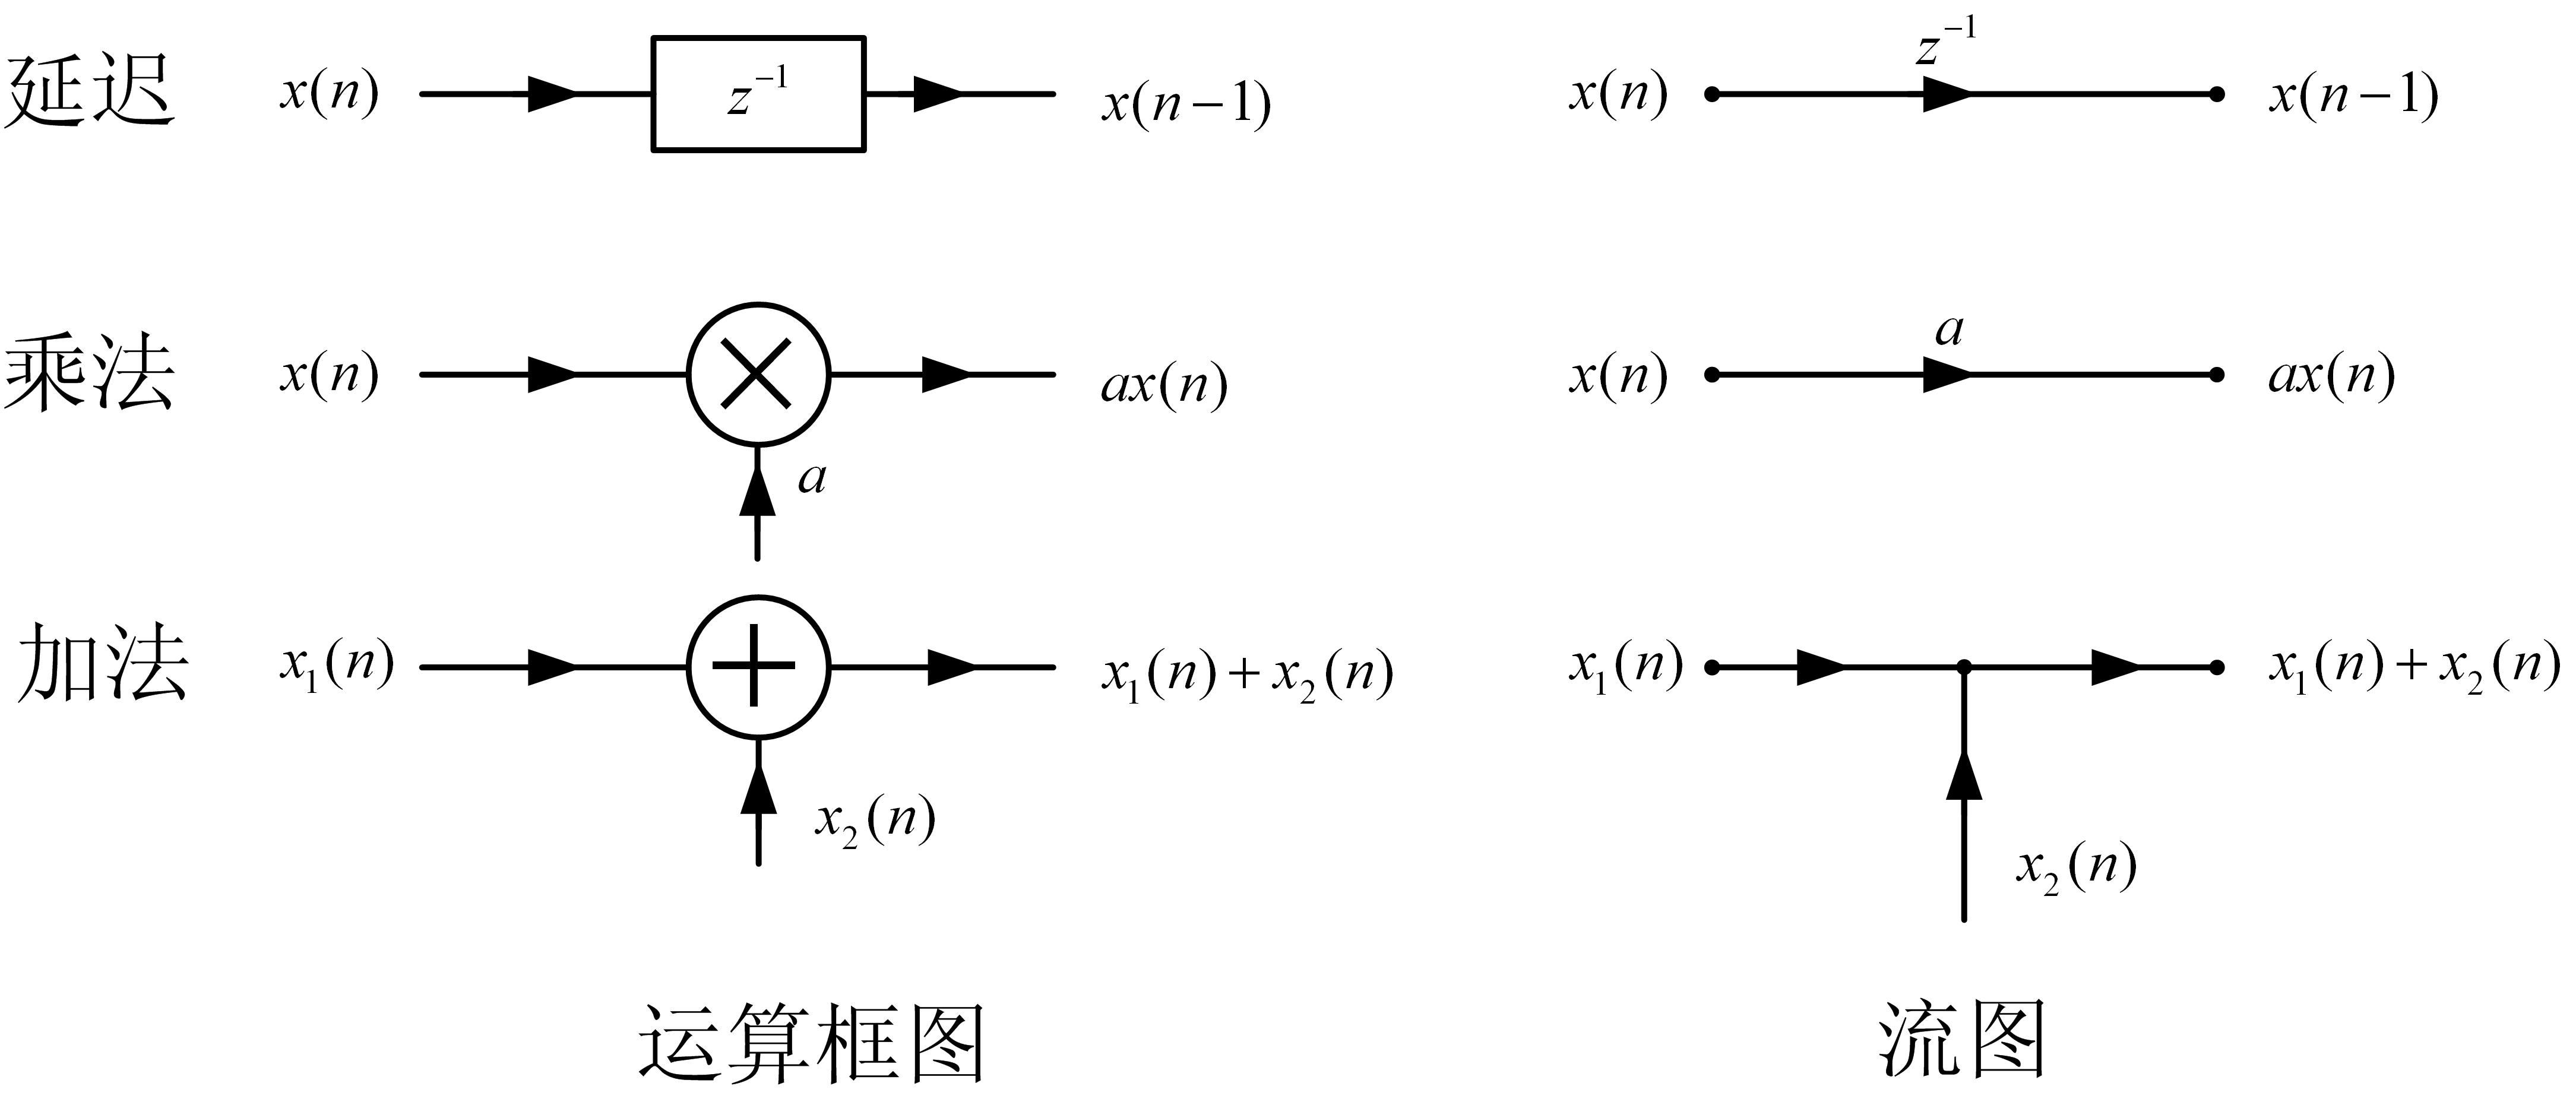
\includegraphics[width=0.8\textwidth]{jibenliutu.jpg}
  %\caption{三种基本运算的流图表示}
  \label{graph:chp5jibenliutu}
\end{figure}
\begin{enumerate}
  \item $z^{-1}$和系数a作为支路增益写在支路箭头旁边,箭头表示信号流动方向。
  \item 两个信号相加,用一个圆点表示,称为网络节点。
  %\item 输入$x(n)$的节点称为源节点或输入节点
\end{enumerate}
\end{frame}
%%%%%%%%%%%%%%%%%%%%%%%%%%%%%%%%%%%%%%%%%%%%%%%%%%%%%%%%%%%%%%%%%%%%%%%%%%%%%%%%%%%%%%%%%%%%%%%%%%%%%%%%%%%%%%%%%%%%%%%%%%%%%%%%%%%%
%%%%%
%%%%%
%%%%%%%%%%%%%%%%%%%%%%%%%%%%%%%%%%%%%%%%%%%%%%%%%%%%%%%%%%%%%%%%%%%%%%%%%%%%%%%%%%%%%%%%%%%%%%%%%%%%%%%%%%%%%%%%%%%%%%%%%%%%%%%%%%%%
%\begin{frame}[allowframebreaks]\frametitle{用信号流图表示网络结构}%[allowframebreaks]
%基本信号流图
%\begin{enumerate}
%  \item 信号流图中所有支路都是基本支路,即支路增益是常数或$z^{-1}$
%  \item 流图环路中必须存在延迟支路;
%  \item 节点和支路的数目是有限的。
%\end{enumerate}
%\end{frame}
%%%%%%%%%%%%%%%%%%%%%%%%%%%%%%%%%%%%%%%%%%%%%%%%%%%%%%%%%%%%%%%%%%%%%%%%%%%%%%%%%%%%%%%%%%%%%%%%%%%%%%%%%%%%%%%%%%%%%%%%%%%%%%%%%%%%
%%%%%
%%%%%
%%%%%%%%%%%%%%%%%%%%%%%%%%%%%%%%%%%%%%%%%%%%%%%%%%%%%%%%%%%%%%%%%%%%%%%%%%%%%%%%%%%%%%%%%%%%%%%%%%%%%%%%%%%%%%%%%%%%%%%%%%%%%%%%%%%%
\begin{frame}[allowframebreaks]\frametitle{用信号流图表示网络结构}%[allowframebreaks]
{\heiti 基本信号流图}
\begin{enumerate}
  \item [(1)] 信号流图中所有支路都是基本支路,即支路增益是常数或$z^{-1}$
  \item [(2)] 流图环路中必须存在延迟支路;
  \item [(3)] 节点和支路的数目是有限的。
\end{enumerate}

\begin{example}
\label{exam:ch5exam1}
设%\mbox{设:}
$$\quad\quad\quad\quad H(z)=\frac{Y(z)}{X(z)}= \frac{b_0+b_1z^{-1}+b_2z^{-2}}{1+a_1z^{-1}+a_2z^{-2}}$$
试画出其基本信号流图。
\end{example}
\newpage
根据$H(z)$的表达式,有:
$$\quad\quad           Y(z)=(b_0+b_1z^{-1}+b_2z^{-2})\frac{X(z)}{1+a_1z^{-1}+a_2z^{-2}}$$
$$\mbox{令:}\quad\quad\quad\quad W(z)=\frac{X(z)}{1+a_1z^{-1}+a_2z^{-2}}\quad\quad\quad$$
$$\mbox{有:}\quad\quad\quad\quad Y(z)=(b_0+b_1z^{-1}+b_2z^{-2})W(z)$$

变换$W(z)$后有:

$$W(z)=X(z)-a_1W(z)z^{-1}-a_2W(z)z^{-2}$$

\end{frame}
%%%%%%%%%%%%%%%%%%%%%%%%%%%%%%%%%%%%%%%%%%%%%%%%%%%%%%%%%%%%%%%%%%%%%%%%%%%%%%%%%%%%%%%%%%%%%%%%%%%%%%%%%%%%%%%%%%%%%%%%%%%%%%%%%%%%
%%%%%
%%%%%
%%%%%%%%%%%%%%%%%%%%%%%%%%%%%%%%%%%%%%%%%%%%%%%%%%%%%%%%%%%%%%%%%%%%%%%%%%%%%%%%%%%%%%%%%%%%%%%%%%%%%%%%%%%%%%%%%%%%%%%%%%%%%%%%%%%%
\begin{frame}\frametitle{}%[allowframebreaks]
$$W(z)=X(z)-a_1W(z)z^{-1}-a_2W(z)z^{-2}$$
$$Y(z)=(b_0+b_1z^{-1}+b_2z^{-2})W(z)$$
%其信号流图如图(\ref{graph:ch5exam1})所示。
\begin{figure}[h]
  \centering
  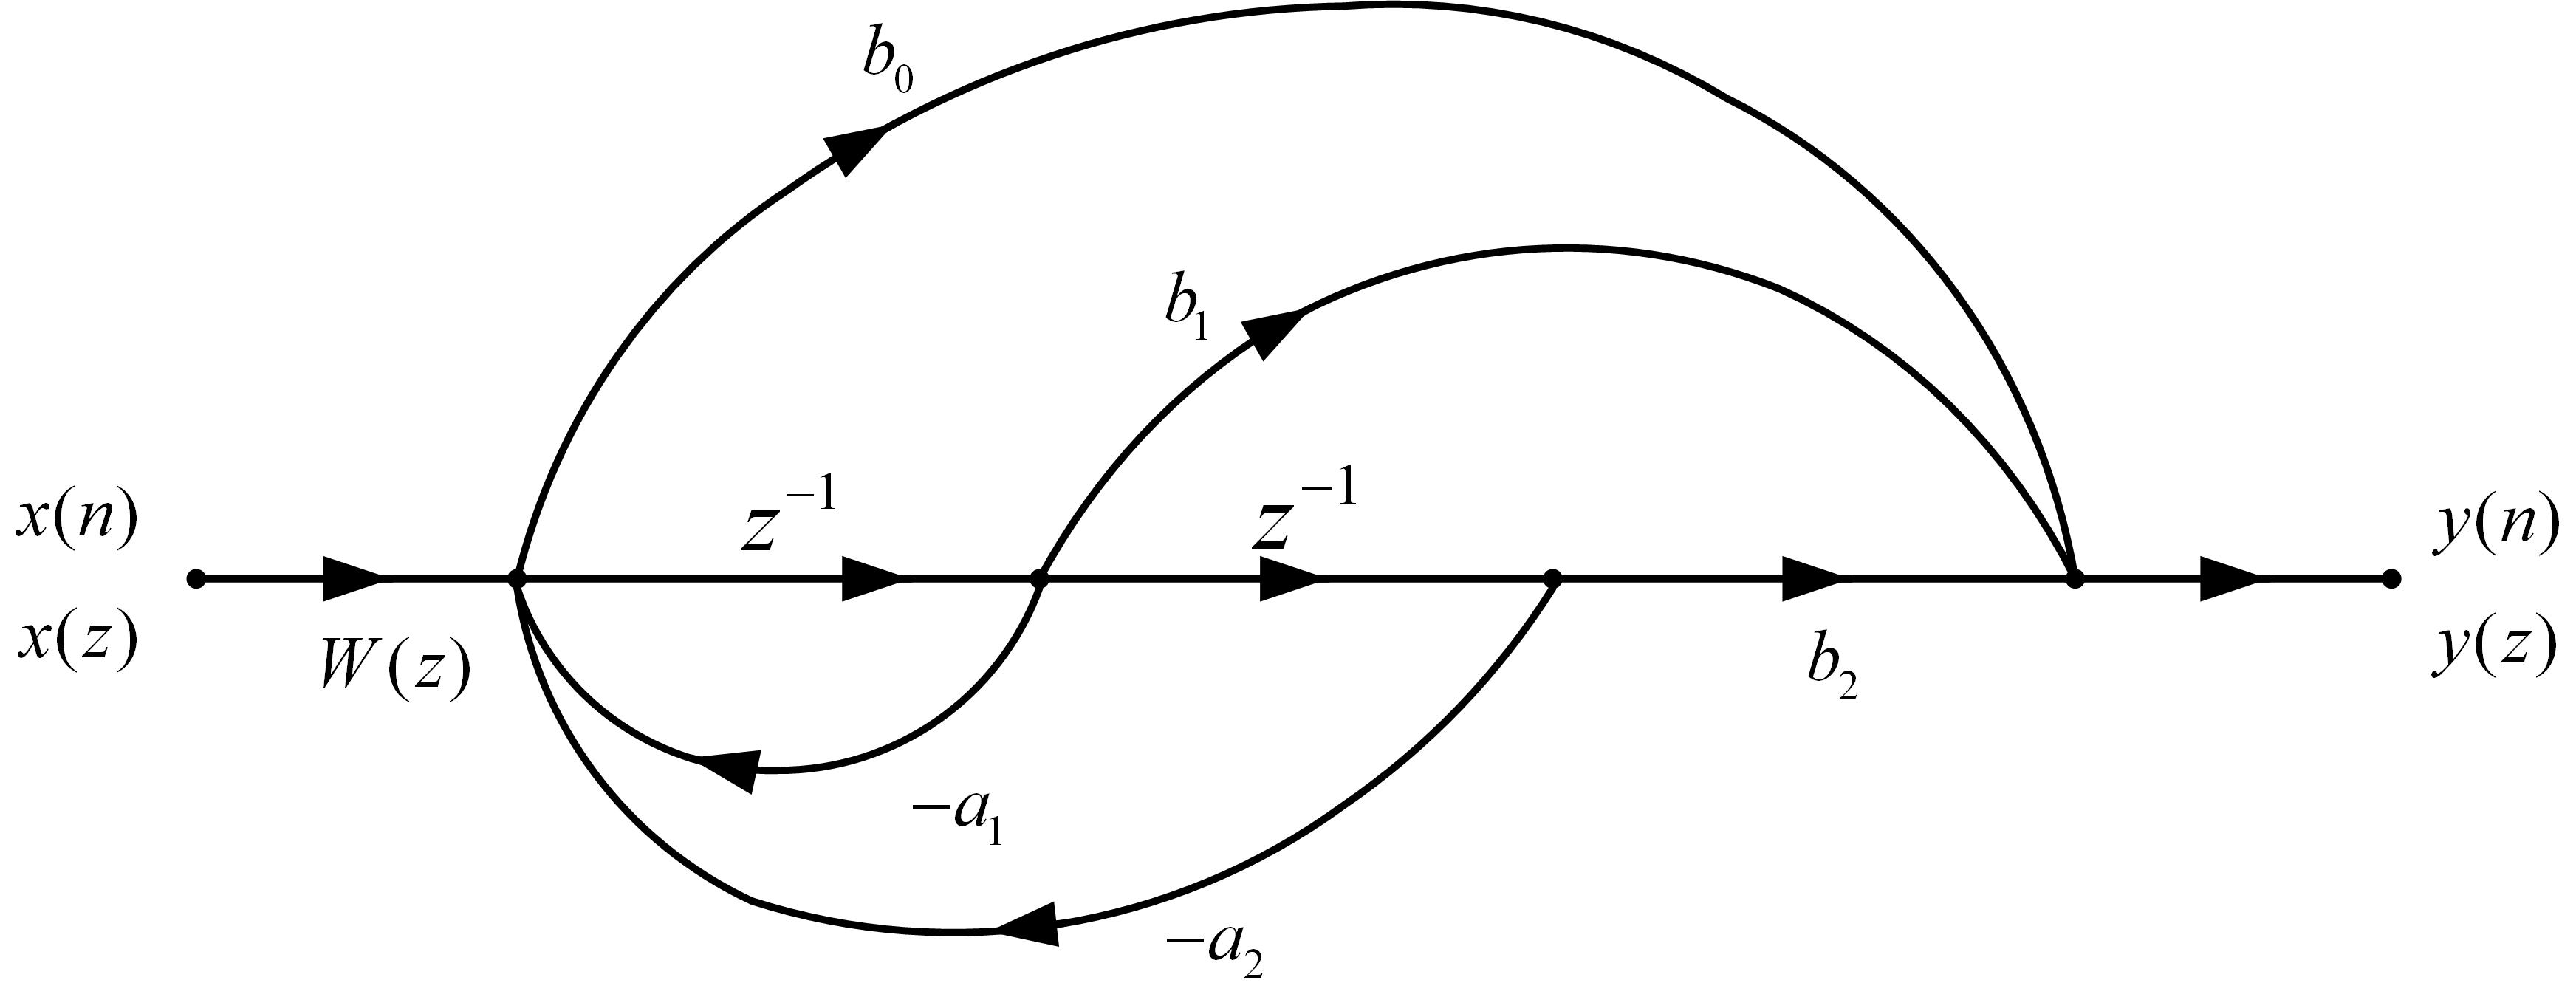
\includegraphics[width=0.8\textwidth]{jbxinhaoliutu.jpg}
  %\caption{例题中对应的基本信号流图}
  \label{graph:ch5exam1}
\end{figure}
\begin{enumerate}
  \item 输入$x(n)$的节点称源节点或输入节点,输出$y(n)$称为吸收节点或输出节点。
  \item 每个节点处的信号称节点变量,{\heiti 节点变量等于所有输入支路信号之和}。
  %\item 节点和支路的数目是有限的。
\end{enumerate}
\end{frame}
%%%%%%%%%%%%%%%%%%%%%%%%%%%%%%%%%%%%%%%%%%%%%%%%%%%%%%%%%%%%%%%%%%%%%%%%%%%%%%%%%%%%%%%%%%%%%%%%%%%%%%%%%%%%%%%%%%%%%%%%%%%%%%%%%%%%
%%%%%
%%%%%
%%%%%%%%%%%%%%%%%%%%%%%%%%%%%%%%%%%%%%%%%%%%%%%%%%%%%%%%%%%%%%%%%%%%%%%%%%%%%%%%%%%%%%%%%%%%%%%%%%%%%%%%%%%%%%%%%%%%%%%%%%%%%%%%%%%%
\begin{frame}[shrink]\frametitle{H(z)的标准形式}%[allowframebreaks]

$$ H(z)=\frac{Y(z)}{X(z)}= \frac{b_0+b_1z^{-1}+b_2z^{-2}}{1+a_1z^{-1}+a_2z^{-2}}$$
\begin{figure}[h]
  \centering
  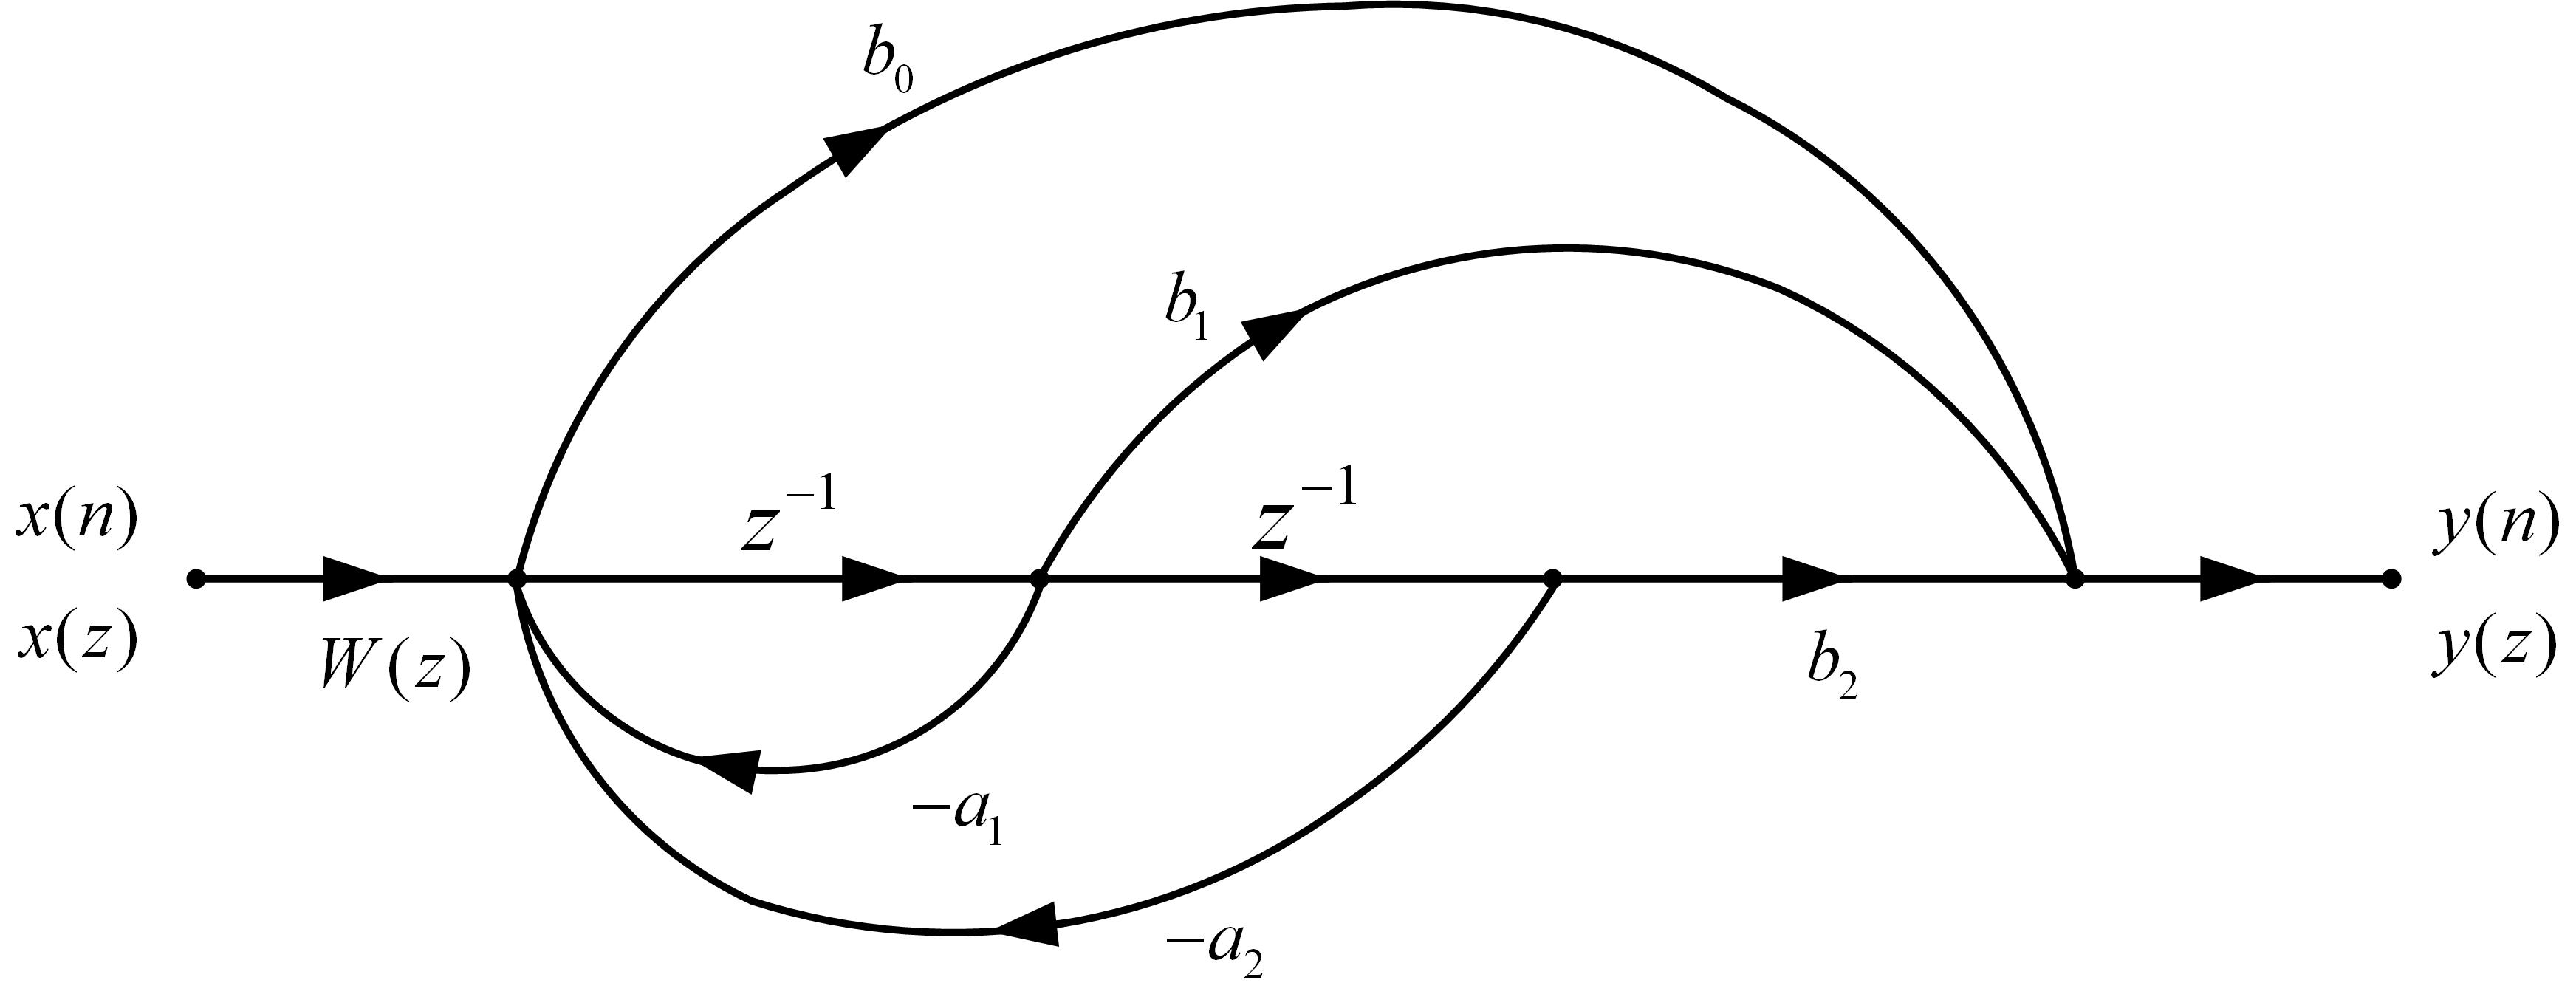
\includegraphics[width=0.7\textwidth]{jbxinhaoliutu.jpg}
  %\caption{例题中对应的基本信号流图}
  \label{graph:ch5exam1}
\end{figure}
\textbf{说明:}
\begin{enumerate}
  \item [(1)] $H(z)$的标准形式为:
  \begin{enumerate}
    \item 分子、分母均为$z^{-1}$的多项式。
    \item 分母中常数项为1。
  \end{enumerate}
  \item [(2)] $H(z)$的\textbf{分子代表前馈支路},\textbf{分母代表反馈支路},且分母中各项系数在图中取负号。
  \item [(3)] 流图中没有标明增益的,其增益为1。
\end{enumerate}
\end{frame}


\subsection{5.2.2 数字滤波器的分类}
%%%%%%%%%%%%%%%%%%%%%%%%%%%%%%%%%%%%%%%%%%%%%%%%%%%%%%%%%%%%%%%%%%%%%%%%%%%%%%%%%%%%%%%%%%%%%%%%%%%%%%%%%%%%%%%%%%%%%%%%%%%%%%%%%%%%
%%%%%
%%%%%
%%%%%%%%%%%%%%%%%%%%%%%%%%%%%%%%%%%%%%%%%%%%%%%%%%%%%%%%%%%%%%%%%%%%%%%%%%%%%%%%%%%%%%%%%%%%%%%%%%%%%%%%%%%%%%%%%%%%%%%%%%%%%%%%%%%%
\begin{frame}[shrink]\frametitle{数字滤波器的分类}%[allowframebreaks]
1、根据数字滤波器的单位取样响应$h(n)$的长度分类
$$
\left\{ \begin{aligned}
\mbox{FIR} &: \mbox{有限长单位脉冲响应滤波器} \quad\quad\quad\quad\quad\quad\quad\quad\quad\quad\quad\quad\\
\mbox{IIR} &: \mbox{无限长单位脉冲响应滤波器}
\end{aligned} \right.
$$
2、根据数字滤波器的实现方式分类
$$
\left\{ \begin{aligned}
\mbox{递归型} &: \mbox{(有反馈)} \quad\quad\quad\quad\quad\quad\quad\quad\quad\quad\quad\quad\\
\mbox{非递归型} &:\mbox{(无反馈)}
\end{aligned} \right.
$$
\end{frame}
%%%%%%%%%%%%%%%%%%%%%%%%%%%%%%%%%%%%%%%%%%%%%%%%%%%%%%%%%%%%%%%%%%%%%%%%%%%%%%%%%%%%%%%%%%%%%%%%%%%%%%%%%%%%%%%%%%%%%%%%%%%%%%%%%%%%
%%%%%
%%%%%
%%%%%%%%%%%%%%%%%%%%%%%%%%%%%%%%%%%%%%%%%%%%%%%%%%%%%%%%%%%%%%%%%%%%%%%%%%%%%%%%%%%%%%%%%%%%%%%%%%%%%%%%%%%%%%%%%%%%%%%%%%%%%%%%%%%%
\begin{frame}[shrink]\frametitle{FIR-DF(有限长单位脉冲响应数字滤波器)}%[allowframebreaks]
\vspace{-0.4cm}
$$\mbox{差分方程}\quad\quad y(n)=\sum_{i=0}^{M}b_ix(n-i)$$
%系统函数:
$$\mbox{系统函数}\quad\quad H(z)=\sum_{i=0}^{M}b_iz^{-i}\quad$$
也就是系统函数的分母为1,而
$$H(z)=\sum_{n=-\infty}^{\infty}h(n)z^{-n}$$
    $$\mbox{有:}\quad\quad h(n) = \left\{\begin{array}
   {r@{,\quad}l}
   b_n &\mbox{$0\leq n \leq M$}\\
   0&\mbox{其他}
  \end{array} \right.$$
重要特点:\textbf{不存在输出对输入的反馈支路}。
\end{frame}
%%%%%%%%%%%%%%%%%%%%%%%%%%%%%%%%%%%%%%%%%%%%%%%%%%%%%%%%%%%%%%%%%%%%%%%%%%%%%%%%%%%%%%%%%%%%%%%%%%%%%%%%%%%%%%%%%%%%%%%%%%%%%%%%%%%%
%%%%%
%%%%%
%%%%%%%%%%%%%%%%%%%%%%%%%%%%%%%%%%%%%%%%%%%%%%%%%%%%%%%%%%%%%%%%%%%%%%%%%%%%%%%%%%%%%%%%%%%%%%%%%%%%%%%%%%%%%%%%%%%%%%%%%%%%%%%%%%%%
\begin{frame}[shrink]\frametitle{IIR-DF无限长单位脉冲响应数字滤波器}%[allowframebreaks]
%IIR-DF (无限长单位脉冲响应滤波器)
\par 其系统函数的分母不总是为1。
\newline
\par 举例说明:
\begin{example}
\par 设$y(n)=x(n)+ay(n-1)$,且为因果系统,求$h(n)$.
\end{example}

\par 解:
\par 显然有:
$$y(n)=x(n)+\underbrace{ay(n-1)}_{\mbox{对应反馈项}}\quad\quad\quad\quad\mbox{(因果)}$$
$$\therefore \qquad Y(z) = X(z) + az^{-1}Y(z)\qquad\qquad\qquad\qquad\qquad\qquad$$
\end{frame}
%%%%%%%%%%%%%%%%%%%%%%%%%%%%%%%%%%%%%%%%%%%%%%%%%%%%%%%%%%%%%%%%%%%%%%%%%%%%%%%%%%%%%%%%%%%%%%%%%%%%%%%%%%%%%%%%%%%%%%%%%%%%%%%%%%%%
%%%%%
%%%%%
%%%%%%%%%%%%%%%%%%%%%%%%%%%%%%%%%%%%%%%%%%%%%%%%%%%%%%%%%%%%%%%%%%%%%%%%%%%%%%%%%%%%%%%%%%%%%%%%%%%%%%%%%%%%%%%%%%%%%%%%%%%%%%%%%%%%
\begin{frame}[shrink]\frametitle{}%[allowframebreaks]
%      \begin{example}
%      \par 设$y(n)=x(n)+ay(n-1)$,且为因果系统,求$h(n)$.
%      \end{example}
%
%      \par 解:
%      \par 显然有:
%      $$y(n)=x(n)+\underbrace{ay(n-1)}_{\mbox{对应反馈项}}\quad\quad\quad\quad\mbox{(因果)}$$
      注意,对于一般系统的差分方程:
      $$y(n)=\underbrace{\sum_{i=0}^{M}b_ix(n-i)}_{\mbox{前馈项}} - \underbrace{\sum_{i=1}^{N}a_iy(n-i)}_{\mbox{反馈项}}\quad\quad\quad\quad\quad\quad
      \quad\quad\quad\quad\quad$$
      $$H(z)=\frac{1}{1-az^{-1}}= \frac{z}{z-a}\quad\quad\quad\quad\quad\quad\quad\quad\quad\quad\quad\quad$$
      \par 又因为系统为因果,可知$|z|>|a|$
      \par 所以可得
      $$ h(n)=a^nu(n)$$

      \par 只要有反馈,总对应无限长响应滤波器(IIR-DF)
\end{frame}
%%%%%%%%%%%%%%%%%%%%%%%%%%%%%%%%%%%%%%%%%%%%%%%%%%%%%%%%%%%%%%%%%%%%%%%%%%%%%%%%%%%%%%%%%%%%%%%%%%%%%%%%%%%%%%%%%%%%%%%%%%%%%%%%%%%%
%%%%%
%%%%%
%%%%%%%%%%%%%%%%%%%%%%%%%%%%%%%%%%%%%%%%%%%%%%%%%%%%%%%%%%%%%%%%%%%%%%%%%%%%%%%%%%%%%%%%%%%%%%%%%%%%%%%%%%%%%%%%%%%%%%%%%%%%%%%%%%%%
\begin{frame}[shrink]\frametitle{根据数字滤波器的实现方式分类}%[allowframebreaks]
$$
\left\{ \begin{aligned}
\mbox{递归型} &: \mbox{(有反馈)} \quad\quad\quad\quad\quad\quad\quad\quad\quad\quad\quad\quad\\
\mbox{非递归型} &:\mbox{(无反馈)}
\end{aligned} \right.
$$
\end{frame}
%%%%%%%%%%%%%%%%%%%%%%%%%%%%%%%%%%%%%%%%%%%%%%%%%%%%%%%%%%%%%%%%%%%%%%%%%%%%%%%%%%%%%%%%%%%%%%%%%%%%%%%%%%%%%%%%%%%%%%%%%%%%%%%%%%%%
%%%%%
%%%%%
%%%%%%%%%%%%%%%%%%%%%%%%%%%%%%%%%%%%%%%%%%%%%%%%%%%%%%%%%%%%%%%%%%%%%%%%%%%%%%%%%%%%%%%%%%%%%%%%%%%%%%%%%%%%%%%%%%%%%%%%%%%%%%%%%%%%
\begin{frame}\frametitle{非递归型}%[allowframebreaks]
    在网络图中无反馈。
    \begin{example}
    $$y(n)=x(n)+ax(n-1)\quad\quad\quad\quad\quad\quad\quad\quad\quad\quad\quad\quad$$
    \end{example}
    \begin{figure}[h]
    \centering
    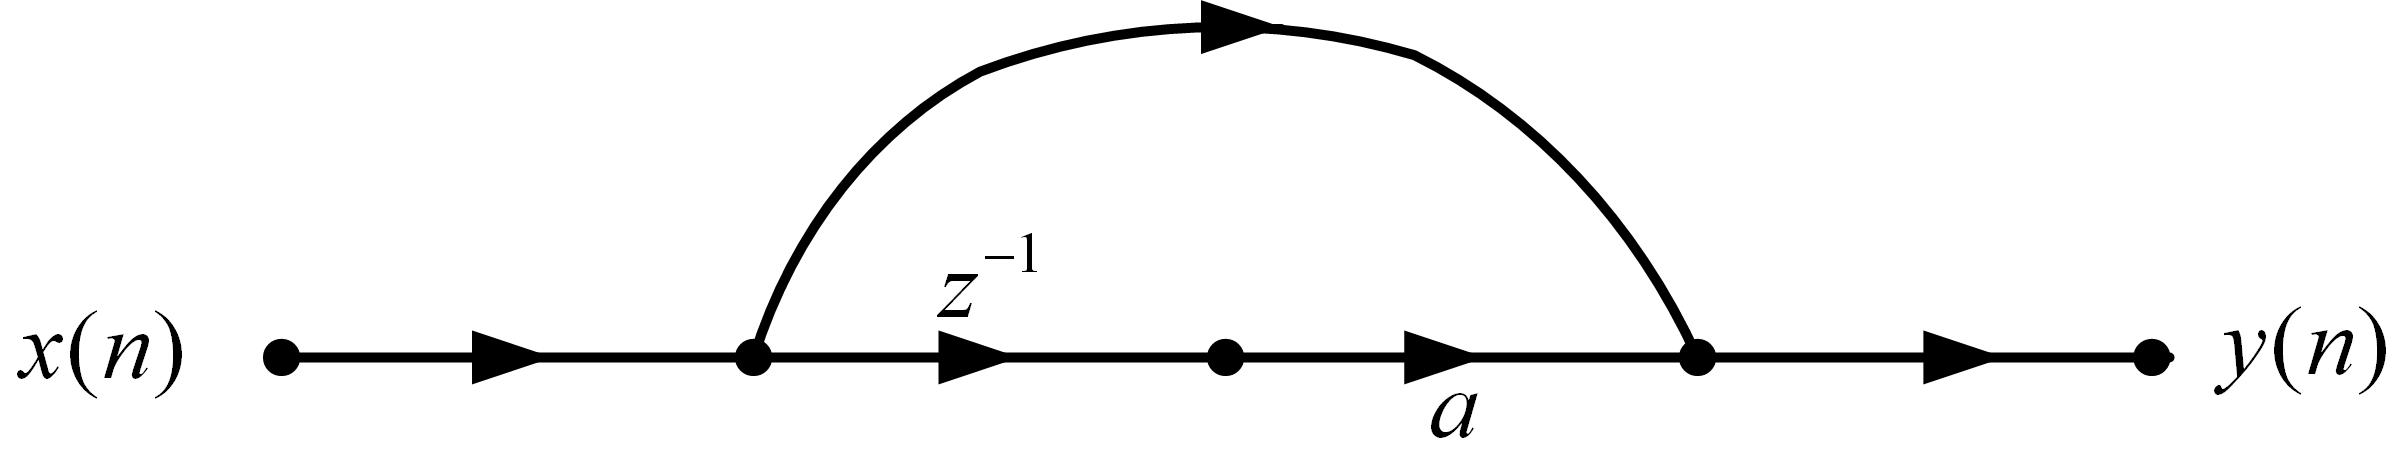
\includegraphics[width=0.8\textwidth]{feidigui.jpg}
    \caption{非递归型数字滤波器的信号流图}
    \label{chp5:jibenliutu}
    \end{figure}
\end{frame}
%%%%%%%%%%%%%%%%%%%%%%%%%%%%%%%%%%%%%%%%%%%%%%%%%%%%%%%%%%%%%%%%%%%%%%%%%%%%%%%%%%%%%%%%%%%%%%%%%%%%%%%%%%%%%%%%%%%%%%%%%%%%%%%%%%%%
%%%%%
%%%%%
%%%%%%%%%%%%%%%%%%%%%%%%%%%%%%%%%%%%%%%%%%%%%%%%%%%%%%%%%%%%%%%%%%%%%%%%%%%%%%%%%%%%%%%%%%%%%%%%%%%%%%%%%%%%%%%%%%%%%%%%%%%%%%%%%%%%
\begin{frame}\frametitle{递归型}%[allowframebreaks]
\par 在网络图中有反馈。
\begin{example}
$$H(z)=\frac{z}{z-a}=\frac{1}{1-az^{-1}}\quad\quad\quad\quad\quad\quad\quad\quad\quad\quad\quad\quad$$
\end{example}
\begin{figure}[h]
\centering
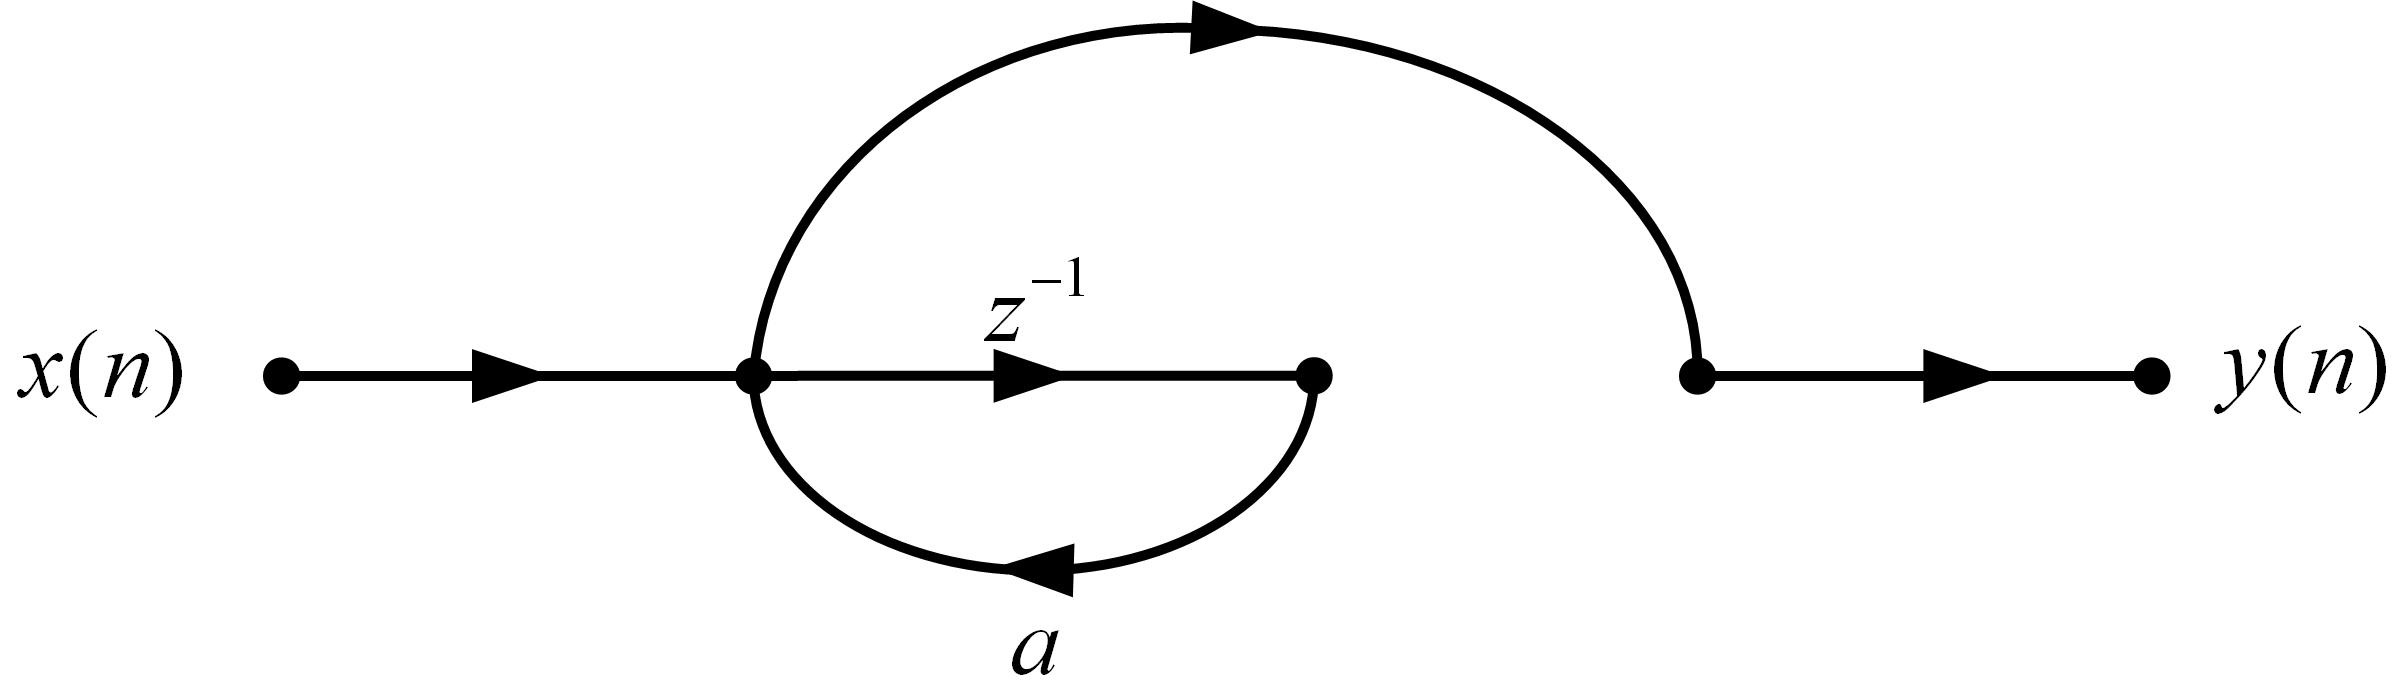
\includegraphics[width=0.8\textwidth]{digui.jpg}
\caption{递归型数字滤波器的信号流图}
\label{chp5:jibenliutu}
\end{figure}
\end{frame}
%%%%%%%%%%%%%%%%%%%%%%%%%%%%%%%%%%%%%%%%%%%%%%%%%%%%%%%%%%%%%%%%%%%%%%%%%%%%%%%%%%%%%%%%%%%%%%%%%%%%%%%%%%%%%%%%%%%%%%%%%%%%%%%%%%%%
%%%%%
%%%%%
%%%%%%%%%%%%%%%%%%%%%%%%%%%%%%%%%%%%%%%%%%%%%%%%%%%%%%%%%%%%%%%%%%%%%%%%%%%%%%%%%%%%%%%%%%%%%%%%%%%%%%%%%%%%%%%%%%%%%%%%%%%%%%%%%%%%
\begin{frame}\frametitle{滤波器的分类}%[allowframebreaks]
\par 目前有了两种分类方法:
$$
\left\{ \begin{aligned}
\mbox{递归型} &\quad   \mbox{和$\quad\quad$非递归型} \quad\quad\quad\quad\quad\quad\quad\quad\quad\quad\quad\quad\\
\mbox{FIR} &\quad \mbox{和$\quad\quad$IIR}
\end{aligned} \right.
$$

但其关系为:
$$
\left\{ \begin{aligned}
\mbox{1)} &\quad \mbox{非递归型一定是FIR} \quad\quad\quad\quad\quad\quad\quad\quad\quad\quad\quad\quad\\
\mbox{2)} &\quad \mbox{IIR一定是递归型结构}
\end{aligned} \right.
$$
\end{frame}
%%%%%%%%%%%%%%%%%%%%%%%%%%%%%%%%%%%%%%%%%%%%%%%%%%%%%%%%%%%%%%%%%%%%%%%%%%%%%%%%%%%%%%%%%%%%%%%%%%%%%%%%%%%%%%%%%%%%%%%%%%%%%%%%%%%%
%%%%%
%%%%%
%%%%%%%%%%%%%%%%%%%%%%%%%%%%%%%%%%%%%%%%%%%%%%%%%%%%%%%%%%%%%%%%%%%%%%%%%%%%%%%%%%%%%%%%%%%%%%%%%%%%%%%%%%%%%%%%%%%%%%%%%%%%%%%%%%%%
\begin{frame}[shrink]\frametitle{滤波器的分类}%[allowframebreaks]
\par 因为有一些FIR-DF也能用递归型网络结构实现,如例%\ref{exam:chp5exam5}
%\begin{example}
\label{exam:chp5exam5} $$H(z)=1+z^{-1}+z^{-2}\quad\quad\quad\quad\quad\quad\quad\mbox{为FIR}$$
\begin{figure}[h]
\centering
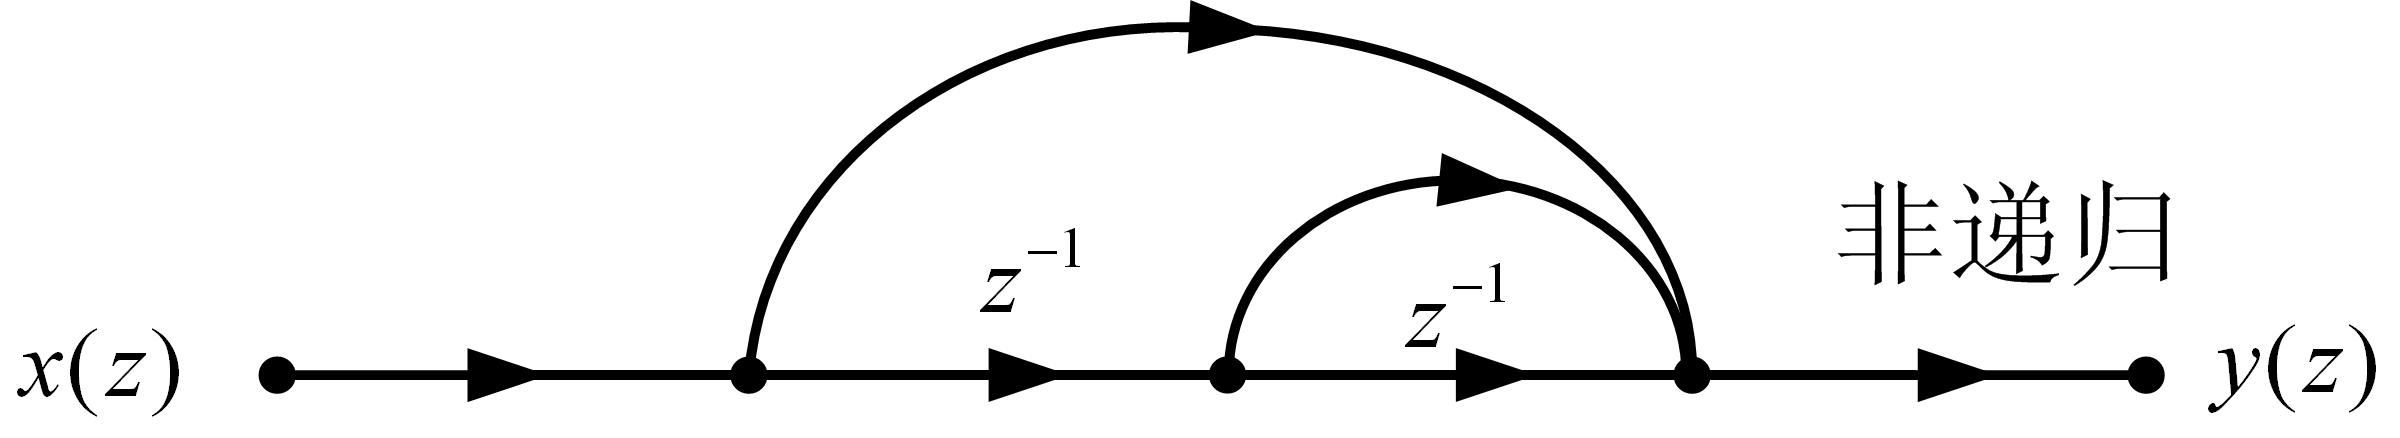
\includegraphics[width=0.6\textwidth]{firfeidigui.jpg}
\caption{非递归型信号流图}
\label{chp5:jibenliutu}
\end{figure}
\vspace{-0.5cm}
\par
$$H(z)=\frac{1-z^{-3}}{1-z^{-1}}\quad\quad\quad\quad\quad\quad\quad\mbox{为FIR}$$
\vspace{-0.3cm}
% $$\mbox{同时可写作}H(z)=\frac{1-z{-3}}{1-z^{-1}}\quad\quad\quad\quad\quad\quad\quad$$
\begin{figure}[h]
\centering
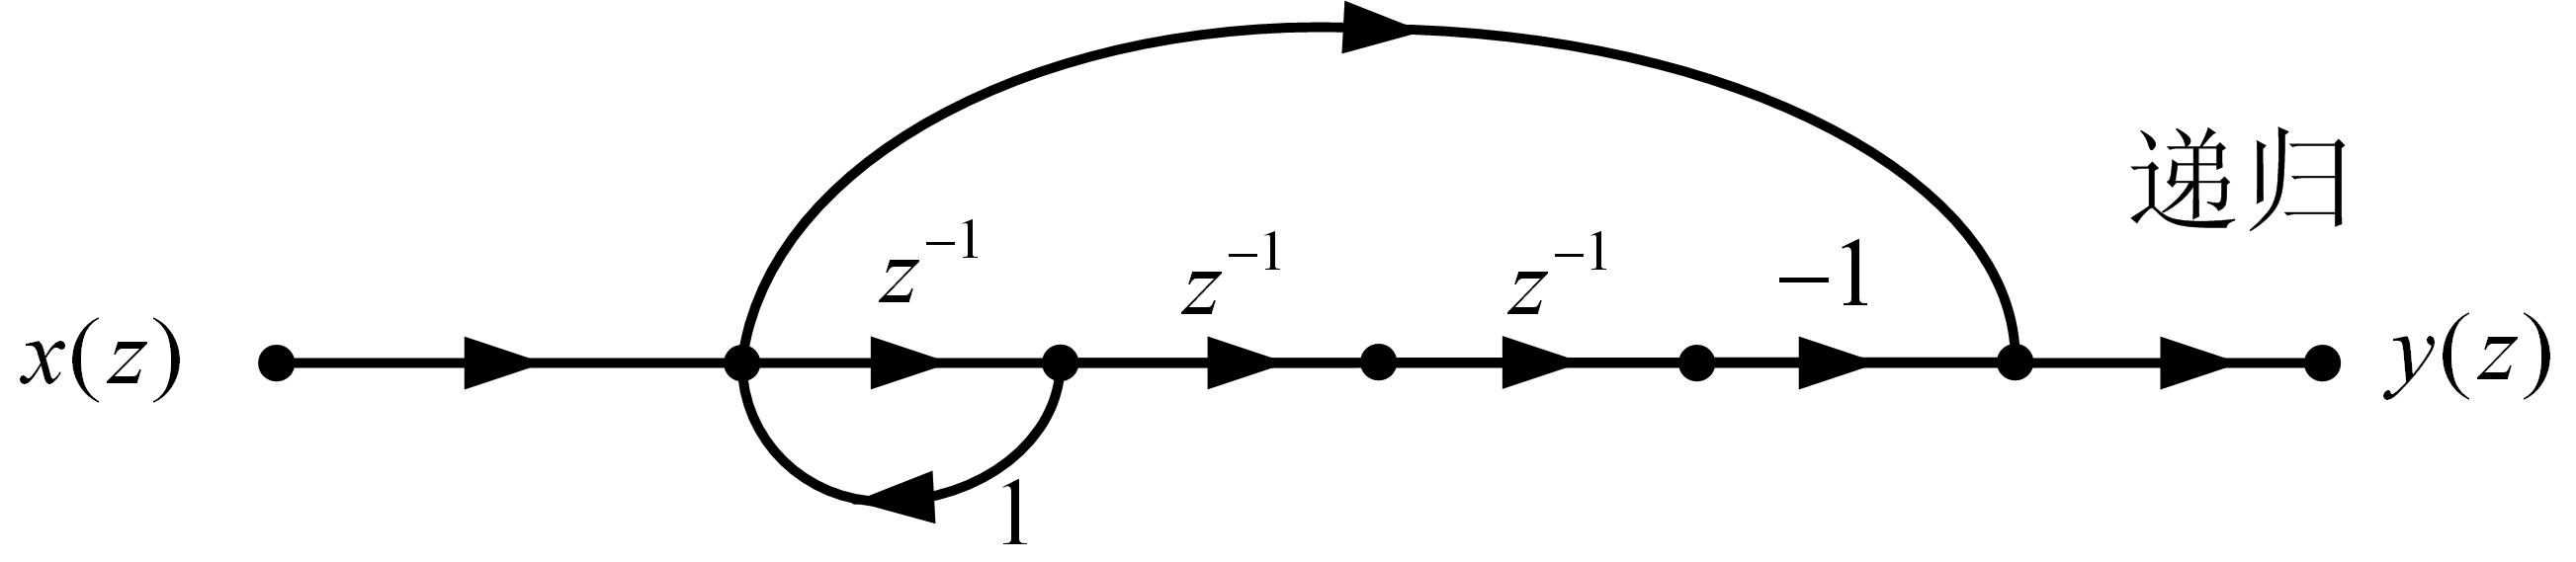
\includegraphics[width=0.6\textwidth]{firdigui.jpg}
\caption{递归型信号流图}
\label{chp5:jibenliutu}
\end{figure}
\vspace{-0.3cm}
\end{frame}
%%%%%%%%%%%%%%%%%%%%%%%%%%%%%%%%%%%%%%%%%%%%%%%%%%%%%%%%%%%%%%%%%%%%%%%%%%%%%%%%%%%%%%%%%%%%%%%%%%%%%%%%%%%%%%%%%%%%%%%%%%%%%%%%%%%%
%%%%%
%%%%%
%%%%%%%%%%%%%%%%%%%%%%%%%%%%%%%%%%%%%%%%%%%%%%%%%%%%%%%%%%%%%%%%%%%%%%%%%%%%%%%%%%%%%%%%%%%%%%%%%%%%%%%%%%%%%%%%%%%%%%%%%%%%%%%%%%%%

\section{5.3 IIR系统的基本网络结构}

\subsection{5.3.1 直接型}
%\subsubsection{直接I型}
%%%%%%%%%%%%%%%%%%%%%%%%%%%%%%%%%%%%%%%%%%%%%%%%%%%%%%%%%%%%%%%%%%%%%%%%%%%%%%%%%%%%%%%%%%%%%%%%%%%%%%%%%%%%%%%%%%%%%%%%%%%%%%%%%%%%
%%%%%
%%%%%
%%%%%%%%%%%%%%%%%%%%%%%%%%%%%%%%%%%%%%%%%%%%%%%%%%%%%%%%%%%%%%%%%%%%%%%%%%%%%%%%%%%%%%%%%%%%%%%%%%%%%%%%%%%%%%%%%%%%%%%%%%%%%%%%%%%%
\begin{frame}[shrink]\frametitle{一、直接I型}%[allowframebreaks]  [shrink]
其N阶差分方程重写如下:
\begin{equation}
\begin{split}
y(n) &= \sum_{i=0}^{M}b_ix(n-i) + \sum_{i=1}^{N}a_iy(n-i)\\
     &= [b_0x(n)+b_1x(n-1)+\cdots+b_Mx(n-M) \\
     &\quad\quad\quad\quad +a_1y(n-1)+\cdots+a_Ny(n-N)]
\end{split}
\end{equation}
对应系统函数为:
$$H(z)=\frac{\sum_{i=0}^{M}b_i z^{-i}}{1-\sum_{i=1}^{N}a_i z^{-i}}$$
\end{frame}
%%%%%%%%%%%%%%%%%%%%%%%%%%%%%%%%%%%%%%%%%%%%%%%%%%%%%%%%%%%%%%%%%%%%%%%%%%%%%%%%%%%%%%%%%%%%%%%%%%%%%%%%%%%%%%%%%%%%%%%%%%%%%%%%%%%%
%%%%%
%%%%%
%%%%%%%%%%%%%%%%%%%%%%%%%%%%%%%%%%%%%%%%%%%%%%%%%%%%%%%%%%%%%%%%%%%%%%%%%%%%%%%%%%%%%%%%%%%%%%%%%%%%%%%%%%%%%%%%%%%%%%%%%%%%%%%%%%%%
\begin{frame}\frametitle{}%[allowframebreaks]  [shrink]

直接I型结构流图如下:
\begin{figure}[h]
\centering
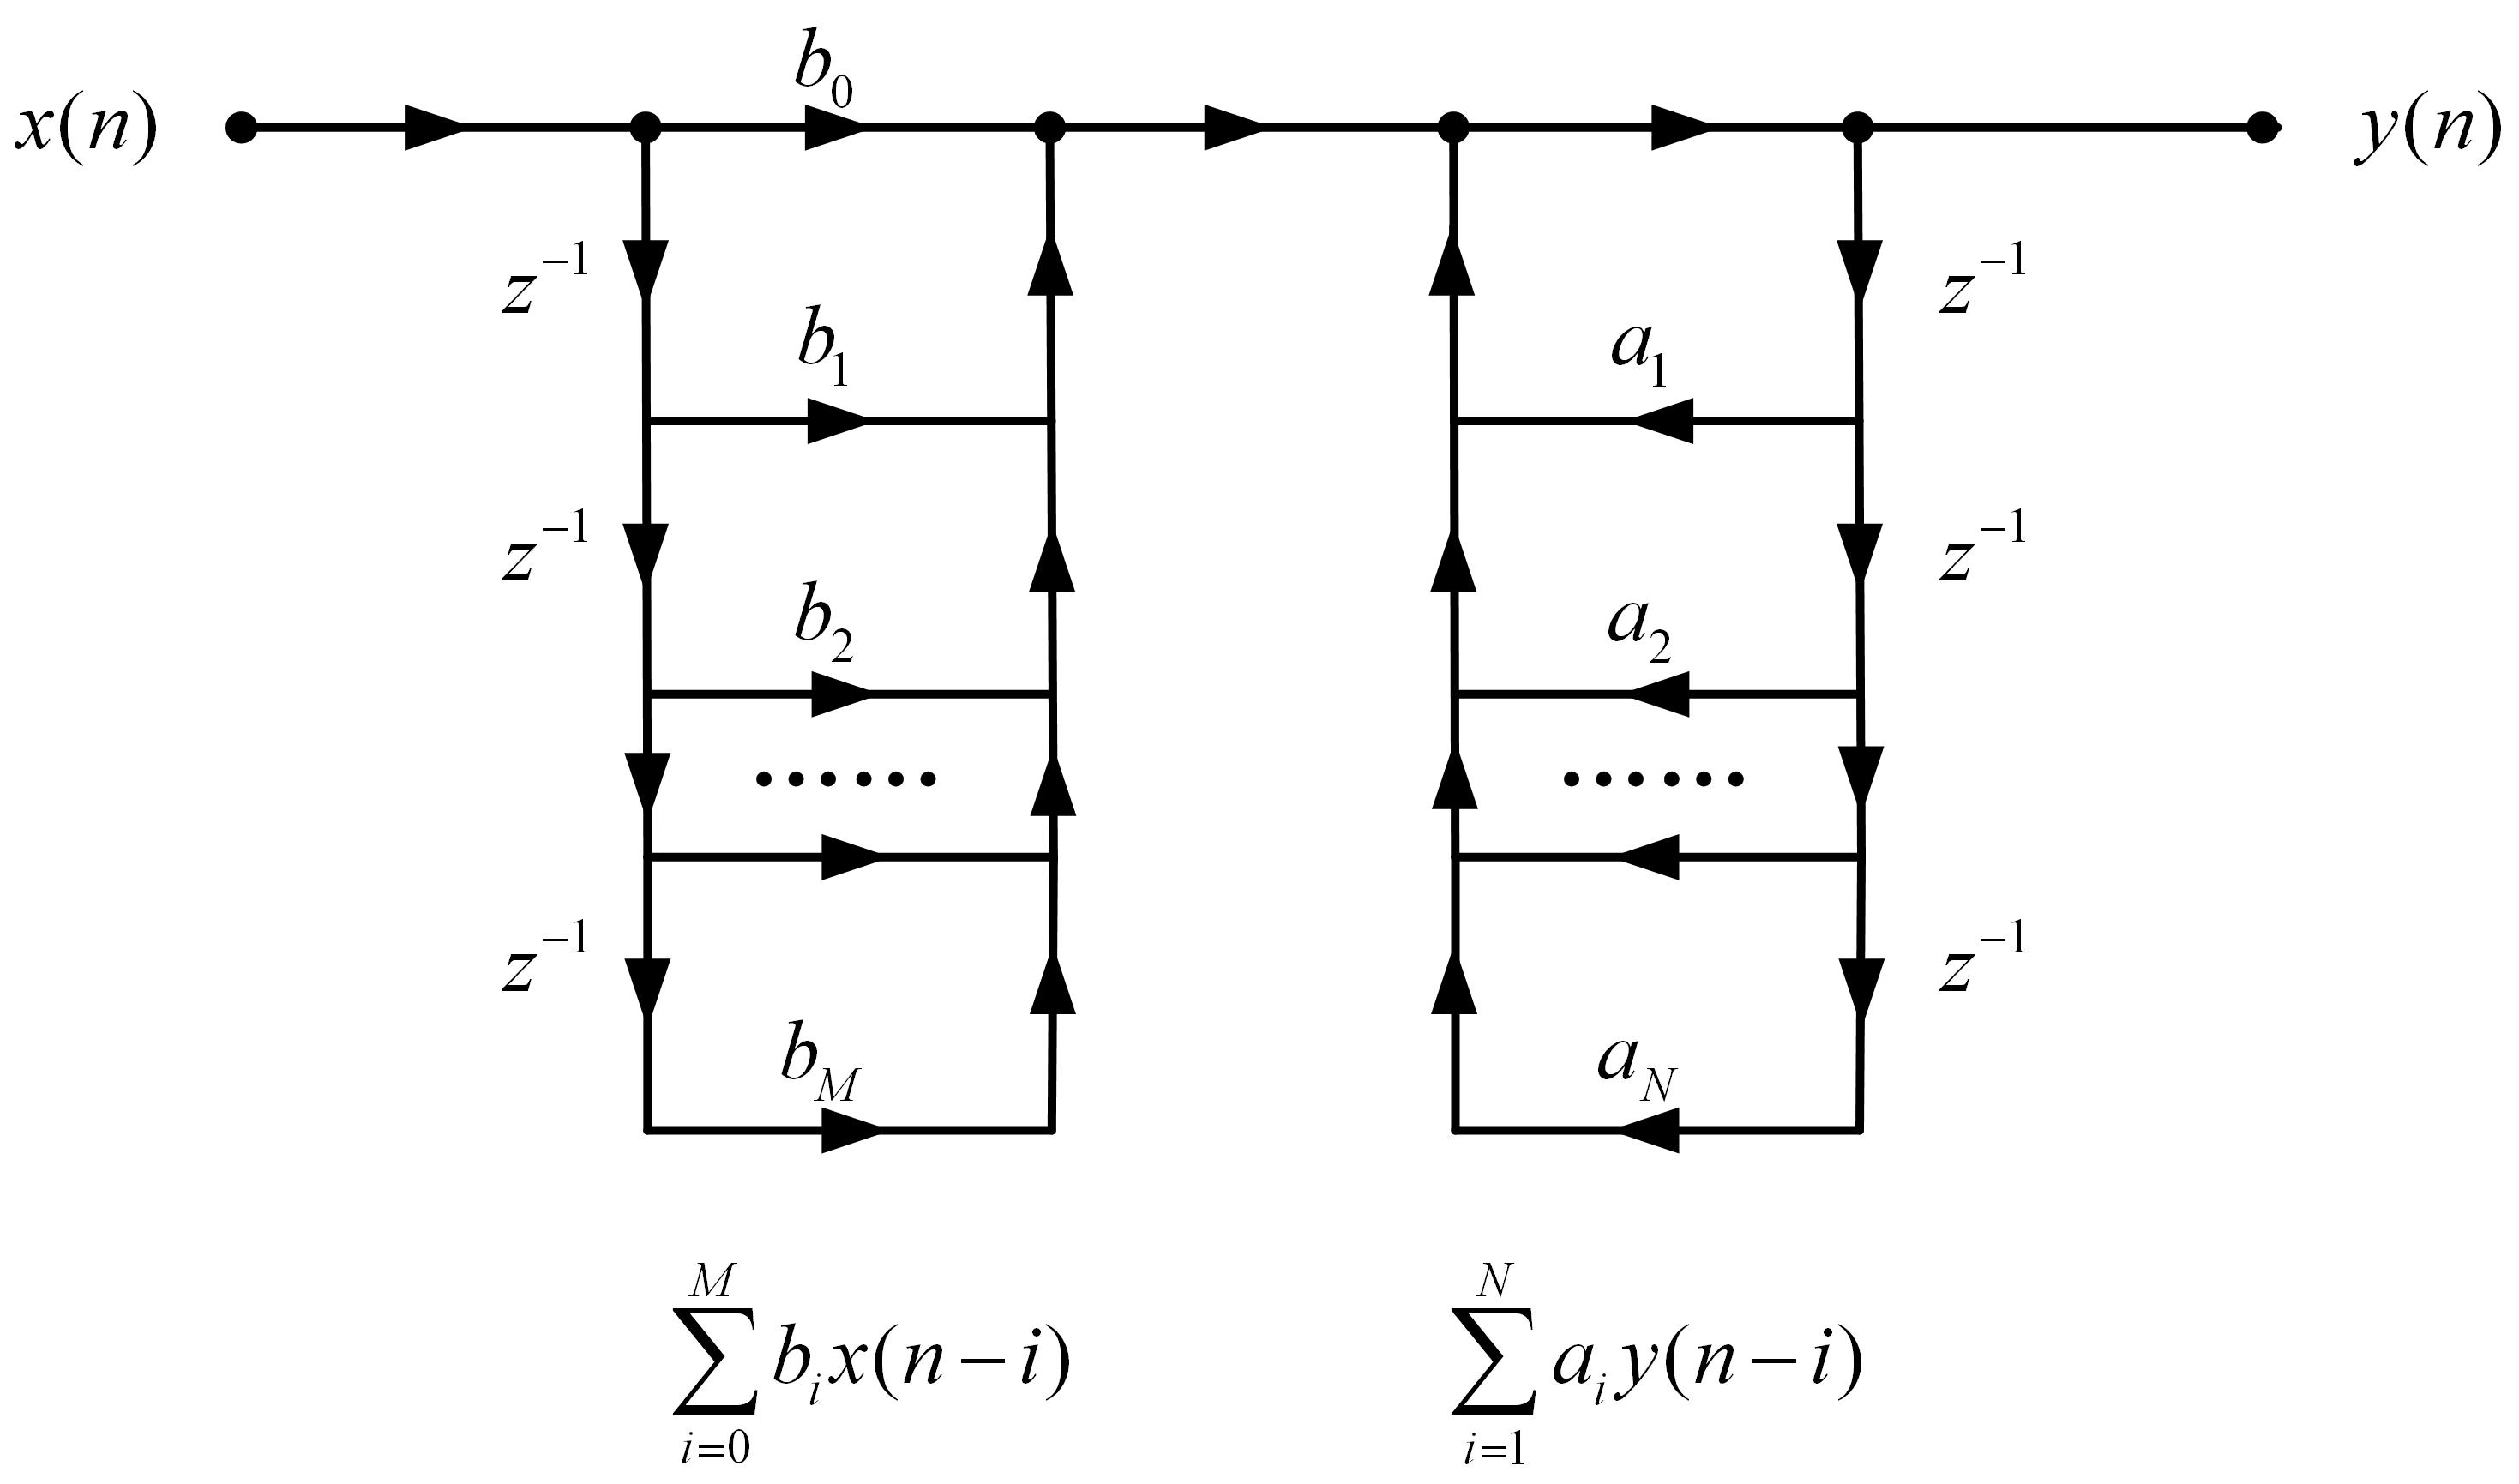
\includegraphics[width=0.95\textwidth]{zhijieyixing.jpg}
%\caption{直接I型结构流图}
%\label{chp5:jibenliutu}
\end{figure}
\end{frame}
%%%%%%%%%%%%%%%%%%%%%%%%%%%%%%%%%%%%%%%%%%%%%%%%%%%%%%%%%%%%%%%%%%%%%%%%%%%%%%%%%%%%%%%%%%%%%%%%%%%%%%%%%%%%%%%%%%%%%%%%%%%%%%%%%%%%
%%%%%
%%%%%
%%%%%%%%%%%%%%%%%%%%%%%%%%%%%%%%%%%%%%%%%%%%%%%%%%%%%%%%%%%%%%%%%%%%%%%%%%%%%%%%%%%%%%%%%%%%%%%%%%%%%%%%%%%%%%%%%%%%%%%%%%%%%%%%%%%%
\begin{frame}[shrink]\frametitle{二、直接II型}%[allowframebreaks]
$$H(z)=H_1(z)\cdot H_2(z)=H_2(z)\cdot H_1(z)$$
\par 直接I型的流图中左右两部分可交换位置,延时支路可以合并,以简化流图结构。
     直接II型结构流图如下:
\begin{figure}[h]
\centering
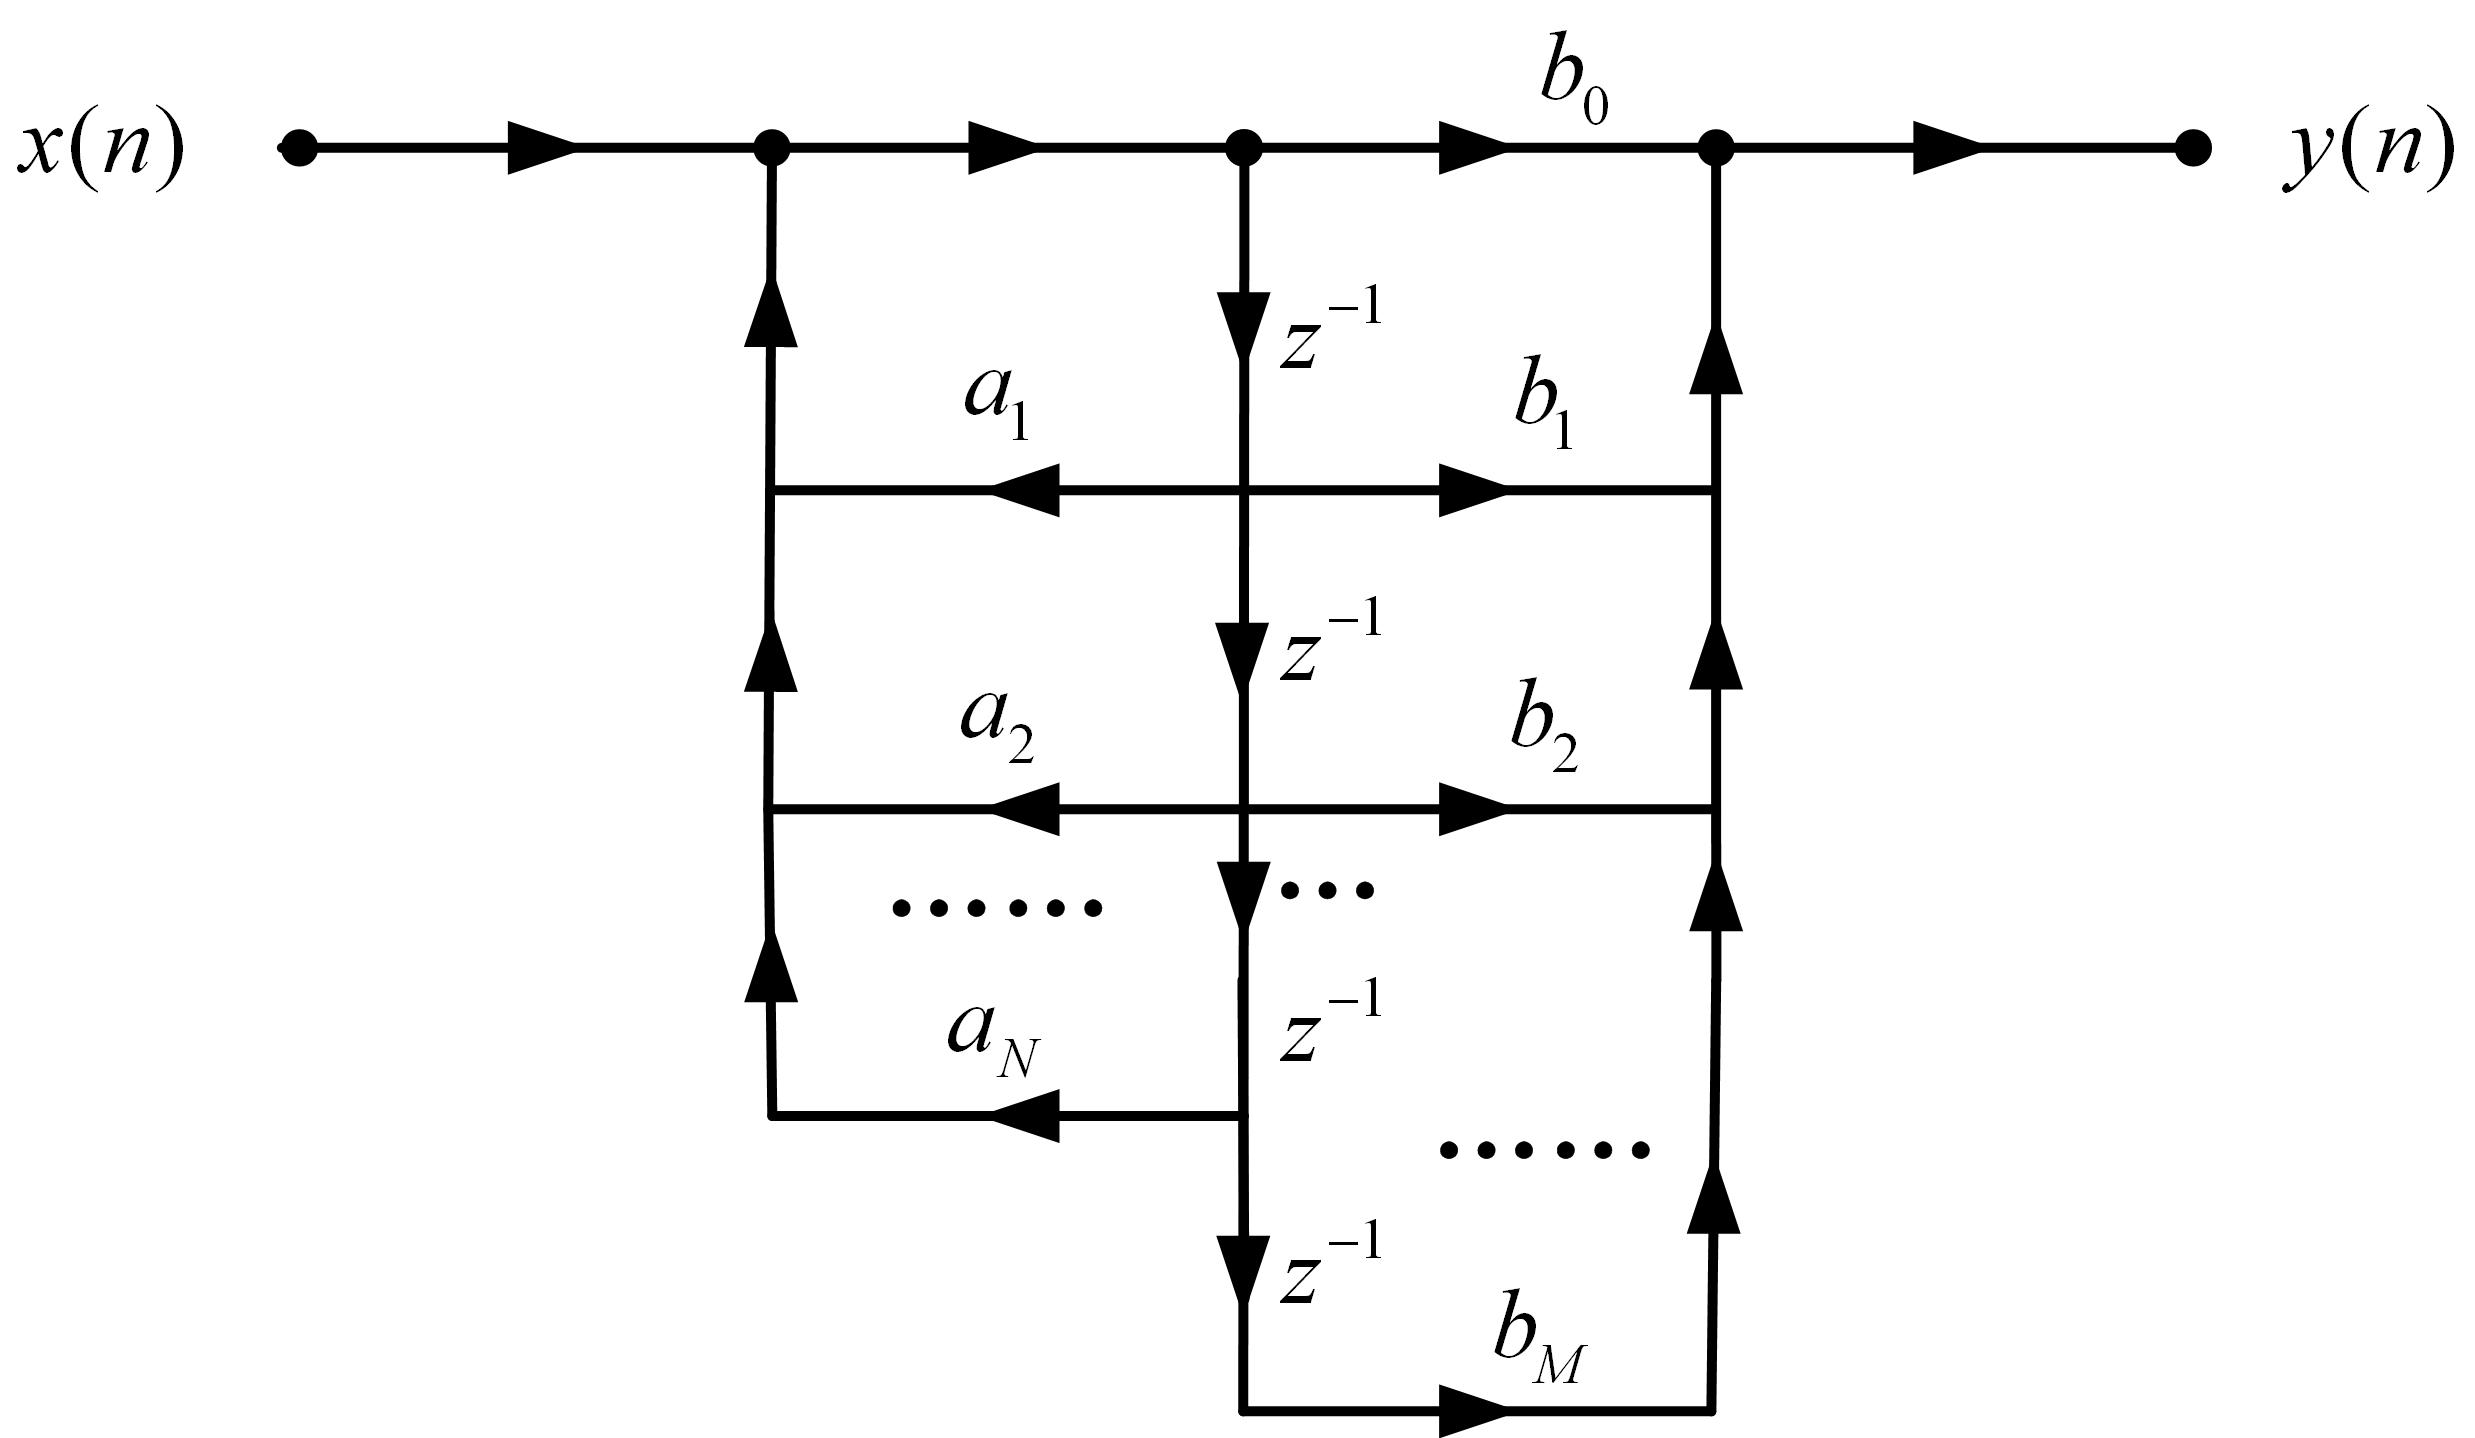
\includegraphics[width=0.75\textwidth]{zhijieerxing.jpg}
%\caption{直接II型结构流图}
\label{chp5:jibenliutu}
\end{figure}
\end{frame}
%%%%%%%%%%%%%%%%%%%%%%%%%%%%%%%%%%%%%%%%%%%%%%%%%%%%%%%%%%%%%%%%%%%%%%%%%%%%%%%%%%%%%%%%%%%%%%%%%%%%%%%%%%%%%%%%%%%%%%%%%%%%%%%%%%%%
%%%%%
%%%%%
%%%%%%%%%%%%%%%%%%%%%%%%%%%%%%%%%%%%%%%%%%%%%%%%%%%%%%%%%%%%%%%%%%%%%%%%%%%%%%%%%%%%%%%%%%%%%%%%%%%%%%%%%%%%%%%%%%%%%%%%%%%%%%%%%%%%
\begin{frame}[shrink]\frametitle{}%[allowframebreaks]
\begin{example}\label{exp:zhijieerxing}
设IIR数字滤波器的系统函数$H(z)$为:
$$H(z)=\frac{8z^3-4z^2+11z-2}{(z-0.25)(z^2-z+0.5)}$$
画出该滤波器的直接型网络结构
\end{example}
$$\mbox{解:}\quad\quad H(z)=\frac{8-4z^{-1}+11z^{-2}-2z^{-3}}{1-1.25z^{-1}+0.75z^{-2}-0.125z^{-3}}
\quad\quad\quad\quad\quad\quad\quad\quad$$
可化为差分方程对比一下。
\begin{equation*}
\begin{split}
y(n) &= 8x(n)-4x(n-1)+11x(n-2)-2x(n-3)\\
     &\quad\quad\quad\quad +1.25y(n-1)-0.75y(n-2)+0.125y(n-3)
\end{split}
\end{equation*}
\end{frame}
%%%%%%%%%%%%%%%%%%%%%%%%%%%%%%%%%%%%%%%%%%%%%%%%%%%%%%%%%%%%%%%%%%%%%%%%%%%%%%%%%%%%%%%%%%%%%%%%%%%%%%%%%%%%%%%%%%%%%%%%%%%%%%%%%%%%
%%%%%
%%%%%
%%%%%%%%%%%%%%%%%%%%%%%%%%%%%%%%%%%%%%%%%%%%%%%%%%%%%%%%%%%%%%%%%%%%%%%%%%%%%%%%%%%%%%%%%%%%%%%%%%%%%%%%%%%%%%%%%%%%%%%%%%%%%%%%%%%%
\begin{frame}[shrink]\frametitle{例题的直接II型结构流图}%[allowframebreaks]
$$H(z)=\frac{8-4z^{-1}+11z^{-2}-2z^{-3}}{1-1.25z^{-1}+0.75z^{-2}-0.125z^{-3}}$$
\begin{figure}[h]
\centering
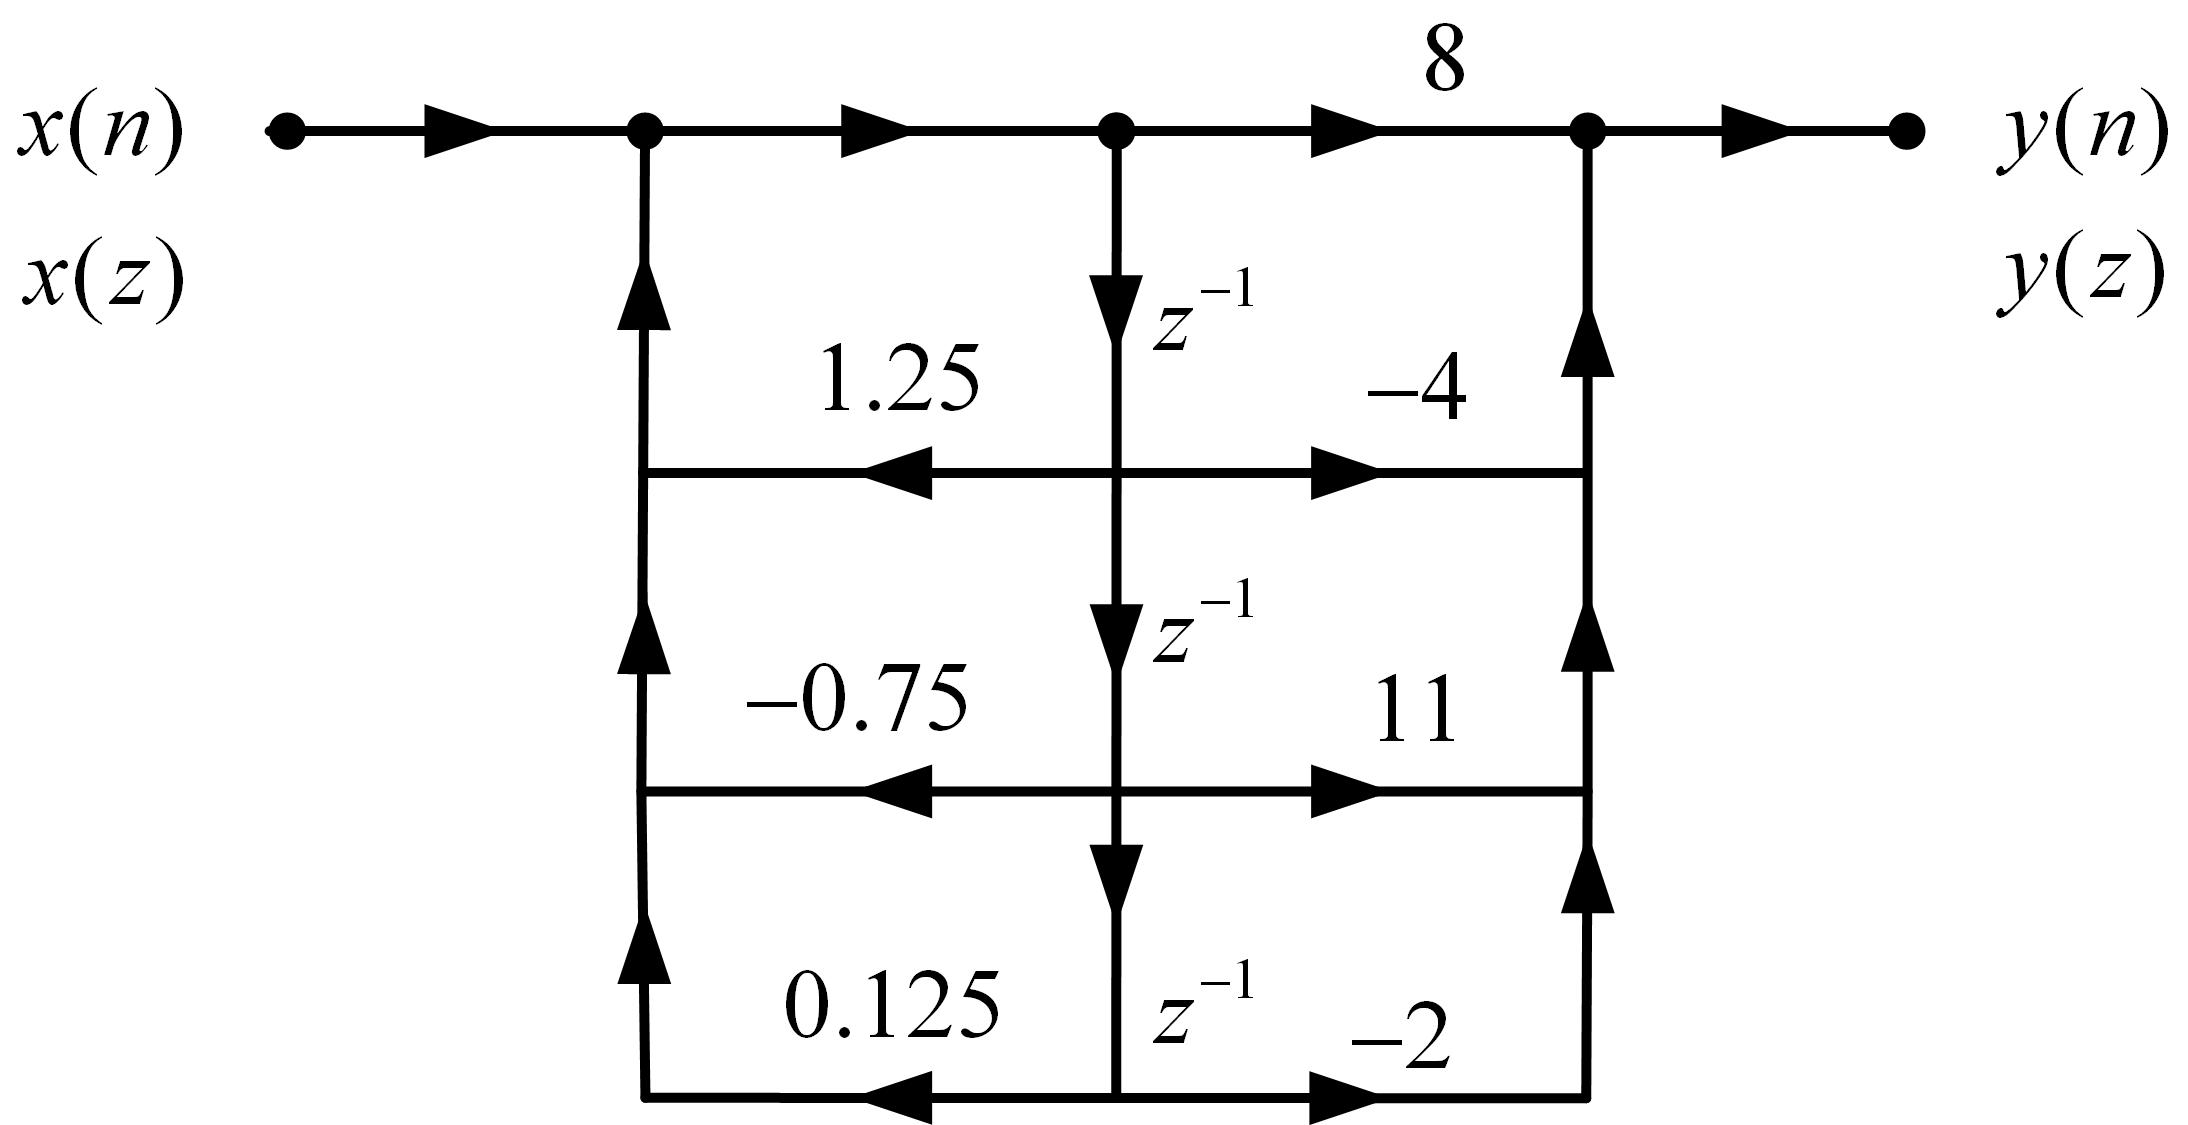
\includegraphics[width=0.80\textwidth]{zhijieerxingli.jpg}
%\caption{例题的直接II型结构流图}
%\label{chp5:jibenliutu}
\end{figure}
\textbf{注意:}
\begin{enumerate}
  \item  $H(z)$的分子代表前馈支路,分母代表反馈支路,且分母中各项系数在图中取负号。
 \end{enumerate}
\end{frame}
%%%%%%%%%%%%%%%%%%%%%%%%%%%%%%%%%%%%%%%%%%%%%%%%%%%%%%%%%%%%%%%%%%%%%%%%%%%%%%%%%%%%%%%%%%%%%%%%%%%%%%%%%%%%%%%%%%%%%%%%%%%%%%%%%%%%
%%%%%
%%%%%
%%%%%%%%%%%%%%%%%%%%%%%%%%%%%%%%%%%%%%%%%%%%%%%%%%%%%%%%%%%%%%%%%%%%%%%%%%%%%%%%%%%%%%%%%%%%%%%%%%%%%%%%%%%%%%%%%%%%%%%%%%%%%%%%%%%%
\subsection{5.3.2 级联型(串联型)}
%%%%%%%%%%%%%%%%%%%%%%%%%%%%%%%%%%%%%%%%%%%%%%%%%%%%%%%%%%%%%%%%%%%%%%%%%%%%%%%%%%%%%%%%%%%%%%%%%%%%%%%%%%%%%%%%%%%%%%%%%%%%%%%%%%%%
%%%%%
%%%%%
%%%%%%%%%%%%%%%%%%%%%%%%%%%%%%%%%%%%%%%%%%%%%%%%%%%%%%%%%%%%%%%%%%%%%%%%%%%%%%%%%%%%%%%%%%%%%%%%%%%%%%%%%%%%%%%%%%%%%%%%%%%%%%%%%%%%
\begin{frame}\frametitle{IIR-DF的级联型网络结构}%[allowframebreaks]
%
系统函数$H(z)$可分解为一阶或二阶的子系统函数积的形式:
$$H(z)=H_1(z)\cdot H_2(z)\cdots \cdot H_k(z)$$
而子系统阶数为1或2,子系统均采用直接型网络结构。
\begin{figure}[h]
\centering
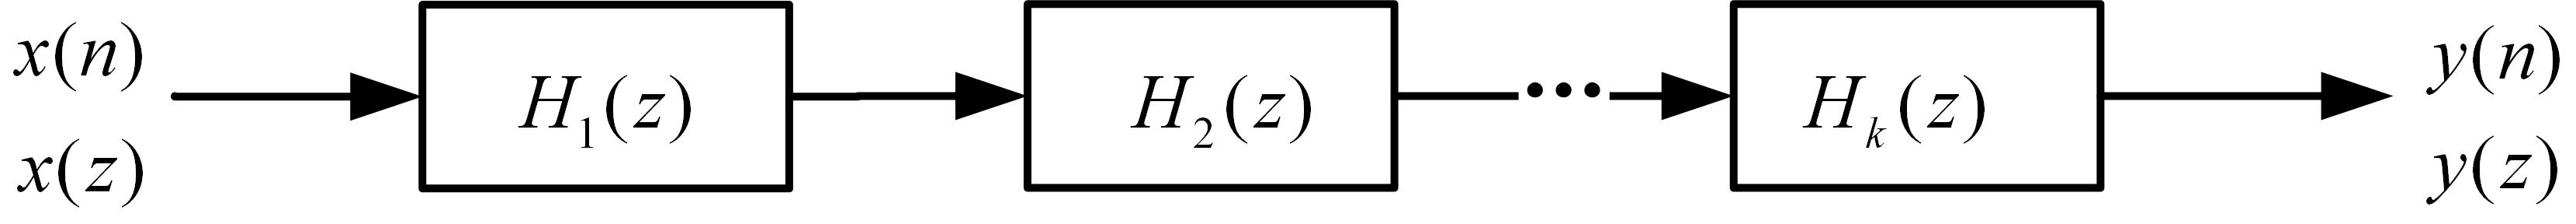
\includegraphics[width=0.9\textwidth]{jilianxing.jpg}
\caption{级联型结构示意图}
%\label{chp5:jibenliutu}
\end{figure}
\end{frame}
%%%%%%%%%%%%%%%%%%%%%%%%%%%%%%%%%%%%%%%%%%%%%%%%%%%%%%%%%%%%%%%%%%%%%%%%%%%%%%%%%%%%%%%%%%%%%%%%%%%%%%%%%%%%%%%%%%%%%%%%%%%%%%%%%%%%
%%%%%
%%%%%
%%%%%%%%%%%%%%%%%%%%%%%%%%%%%%%%%%%%%%%%%%%%%%%%%%%%%%%%%%%%%%%%%%%%%%%%%%%%%%%%%%%%%%%%%%%%%%%%%%%%%%%%%%%%%%%%%%%%%%%%%%%%%%%%%%%%
\subsection{5.3.3 并联型}
%%%%%%%%%%%%%%%%%%%%%%%%%%%%%%%%%%%%%%%%%%%%%%%%%%%%%%%%%%%%%%%%%%%%%%%%%%%%%%%%%%%%%%%%%%%%%%%%%%%%%%%%%%%%%%%%%%%%%%%%%%%%%%%%%%%%
%%%%%
%%%%%
%%%%%%%%%%%%%%%%%%%%%%%%%%%%%%%%%%%%%%%%%%%%%%%%%%%%%%%%%%%%%%%%%%%%%%%%%%%%%%%%%%%%%%%%%%%%%%%%%%%%%%%%%%%%%%%%%%%%%%%%%%%%%%%%%%%%
\begin{frame}\frametitle{IIR-DF的并联型网络结构}%[allowframebreaks]
%
系统函数$H(z)$可分解为一阶或二阶的子系统函数和的形式:
$$H(z)=H_1(z)+ H_2(z)+ \cdots + H_k(z)$$
而子系统阶数为1或2,子系统均采用直接型网络结构。
\begin{figure}[h]
\centering
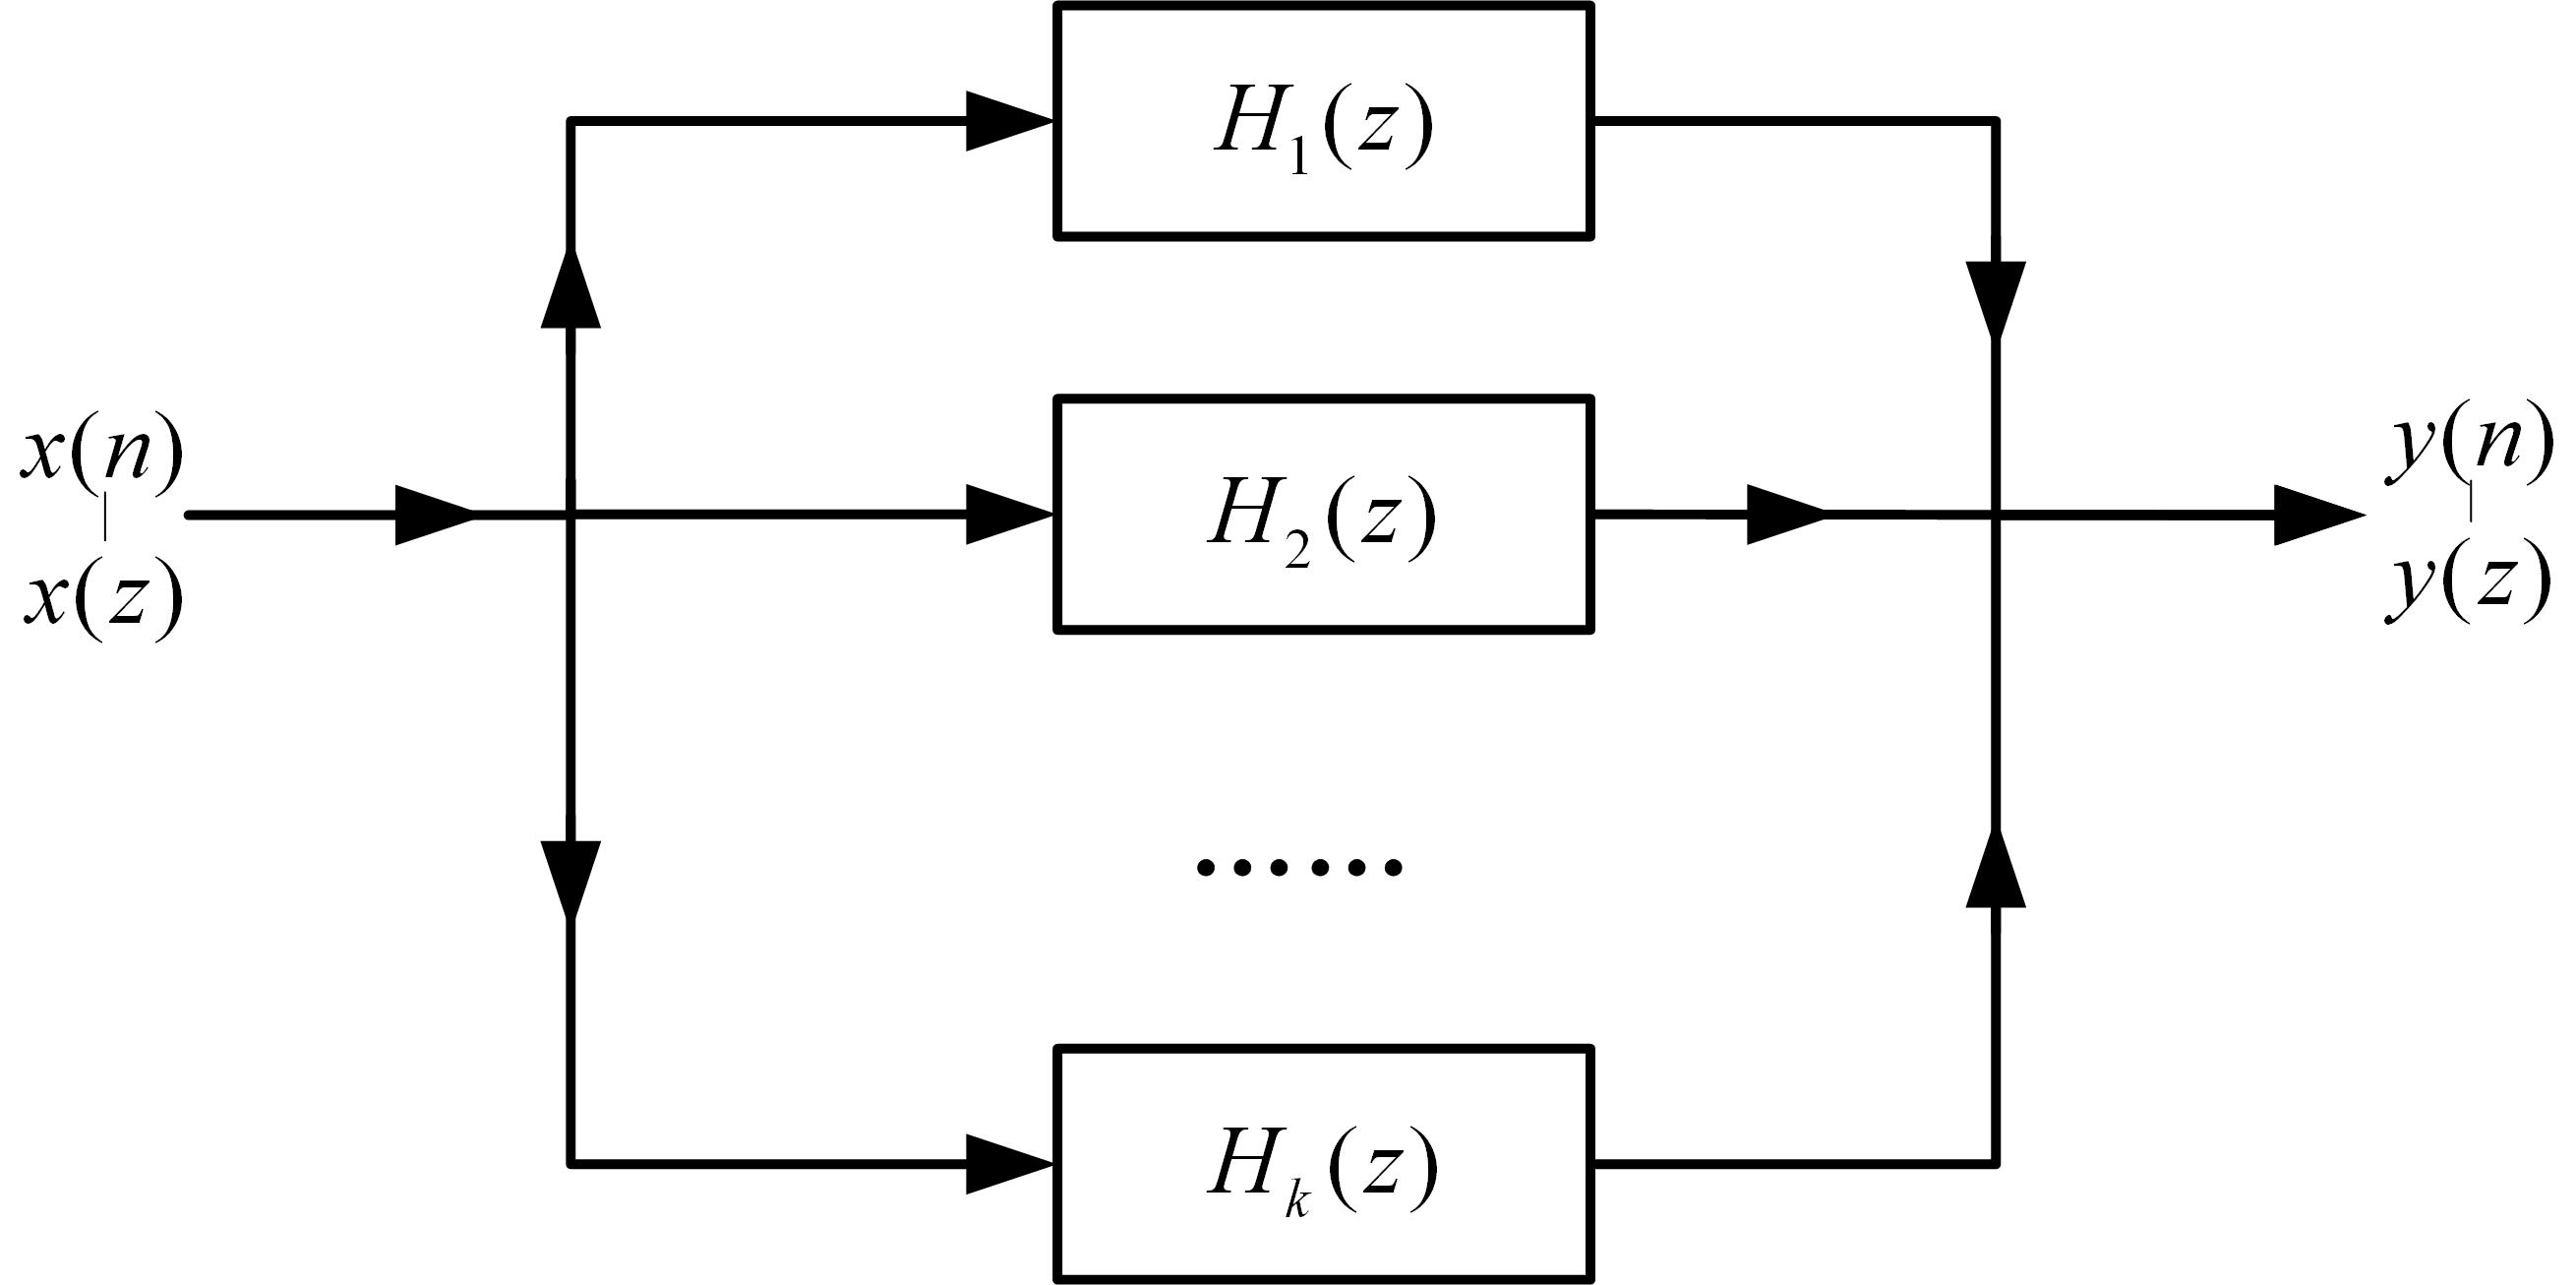
\includegraphics[width=0.7\textwidth]{binglianxing.jpg}
\caption{并联型结构示意图}
%\label{chp5:jibenliutu}
\end{figure}
\end{frame}
%%%%%%%%%%%%%%%%%%%%%%%%%%%%%%%%%%%%%%%%%%%%%%%%%%%%%%%%%%%%%%%%%%%%%%%%%%%%%%%%%%%%%%%%%%%%%%%%%%%%%%%%%%%%%%%%%%%%%%%%%%%%%%%%%%%%
%%%%%
%%%%%
%%%%%%%%%%%%%%%%%%%%%%%%%%%%%%%%%%%%%%%%%%%%%%%%%%%%%%%%%%%%%%%%%%%%%%%%%%%%%%%%%%%%%%%%%%%%%%%%%%%%%%%%%%%%%%%%%%%%%%%%%%%%%%%%%%%%
\begin{frame}\frametitle{}%[allowframebreaks]
\begin{example}\label{exp:jilian}
设系统函数$H(z)$为:
$$H(z)=\frac{8-4z^{-1}+11z^{-2}-2z^{-3}}{1-1.25z^{-1}+0.75z^{-2}-0.125z^{-3}}$$
分别画出其串联型网络结构和并联型网络结构。
\end{example}

\end{frame}
%%%%%%%%%%%%%%%%%%%%%%%%%%%%%%%%%%%%%%%%%%%%%%%%%%%%%%%%%%%%%%%%%%%%%%%%%%%%%%%%%%%%%%%%%%%%%%%%%%%%%%%%%%%%%%%%%%%%%%%%%%%%%%%%%%%%
%%%%%
%%%%%
%%%%%%%%%%%%%%%%%%%%%%%%%%%%%%%%%%%%%%%%%%%%%%%%%%%%%%%%%%%%%%%%%%%%%%%%%%%%%%%%%%%%%%%%%%%%%%%%%%%%%%%%%%%%%%%%%%%%%%%%%%%%%%%%%%%%
\begin{frame}\frametitle{解:(1)串联型结构}%[allowframebreaks]

对其进行因式分解,可得:
\begin{equation}
\begin{split}
H(z) &= \frac{(2-0.379z^{-1})(4-1.24z^{-1}+5.26z^{-2})}{(1-0.25z^{-1})(1-z^{-1}+0.5z^{-2})}\\
     &= \frac{2-0.379z^{-1}}{1-0.25z^{-1}}\cdot\frac{4-1.24z^{-1}+5.26z^{-2})}{1-z^{-1}+0.5z^{-2}}\\
\end{split}
\end{equation}

\begin{figure}[h]
\centering
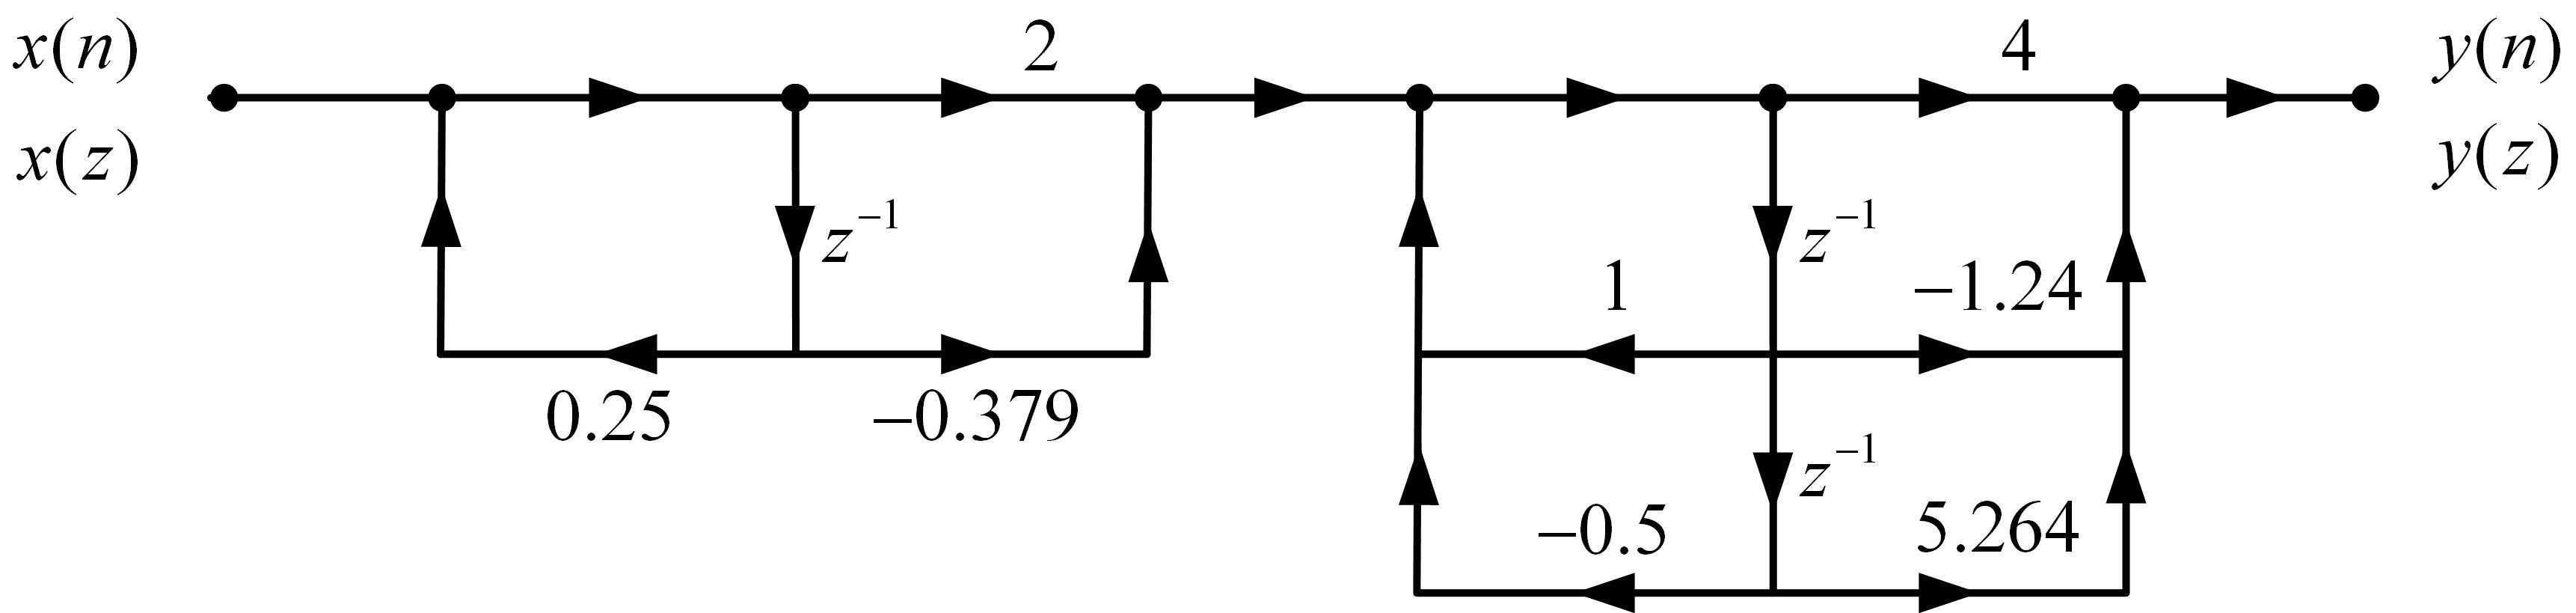
\includegraphics[width=0.95\textwidth]{jilianxingli.jpg}
\caption{例题的级联型结构示意图}
\label{chp5:jibenliutu}
\end{figure}

\end{frame}
%%%%%%%%%%%%%%%%%%%%%%%%%%%%%%%%%%%%%%%%%%%%%%%%%%%%%%%%%%%%%%%%%%%%%%%%%%%%%%%%%%%%%%%%%%%%%%%%%%%%%%%%%%%%%%%%%%%%%%%%%%%%%%%%%%%%
%%%%%
%%%%%
%%%%%%%%%%%%%%%%%%%%%%%%%%%%%%%%%%%%%%%%%%%%%%%%%%%%%%%%%%%%%%%%%%%%%%%%%%%%%%%%%%%%%%%%%%%%%%%%%%%%%%%%%%%%%%%%%%%%%%%%%%%%%%%%%%%%
\begin{frame}\frametitle{(2) 并联型结构}%[allowframebreaks]
对其进行因式分解得:
$$H(z) = 16 +\frac{8}{1-0.5z^{-1}}+\frac{-16 +20z^{-1}}{1-z^{-1}+0.5z^{-2}}$$
\pause
\begin{figure}[h]
\centering
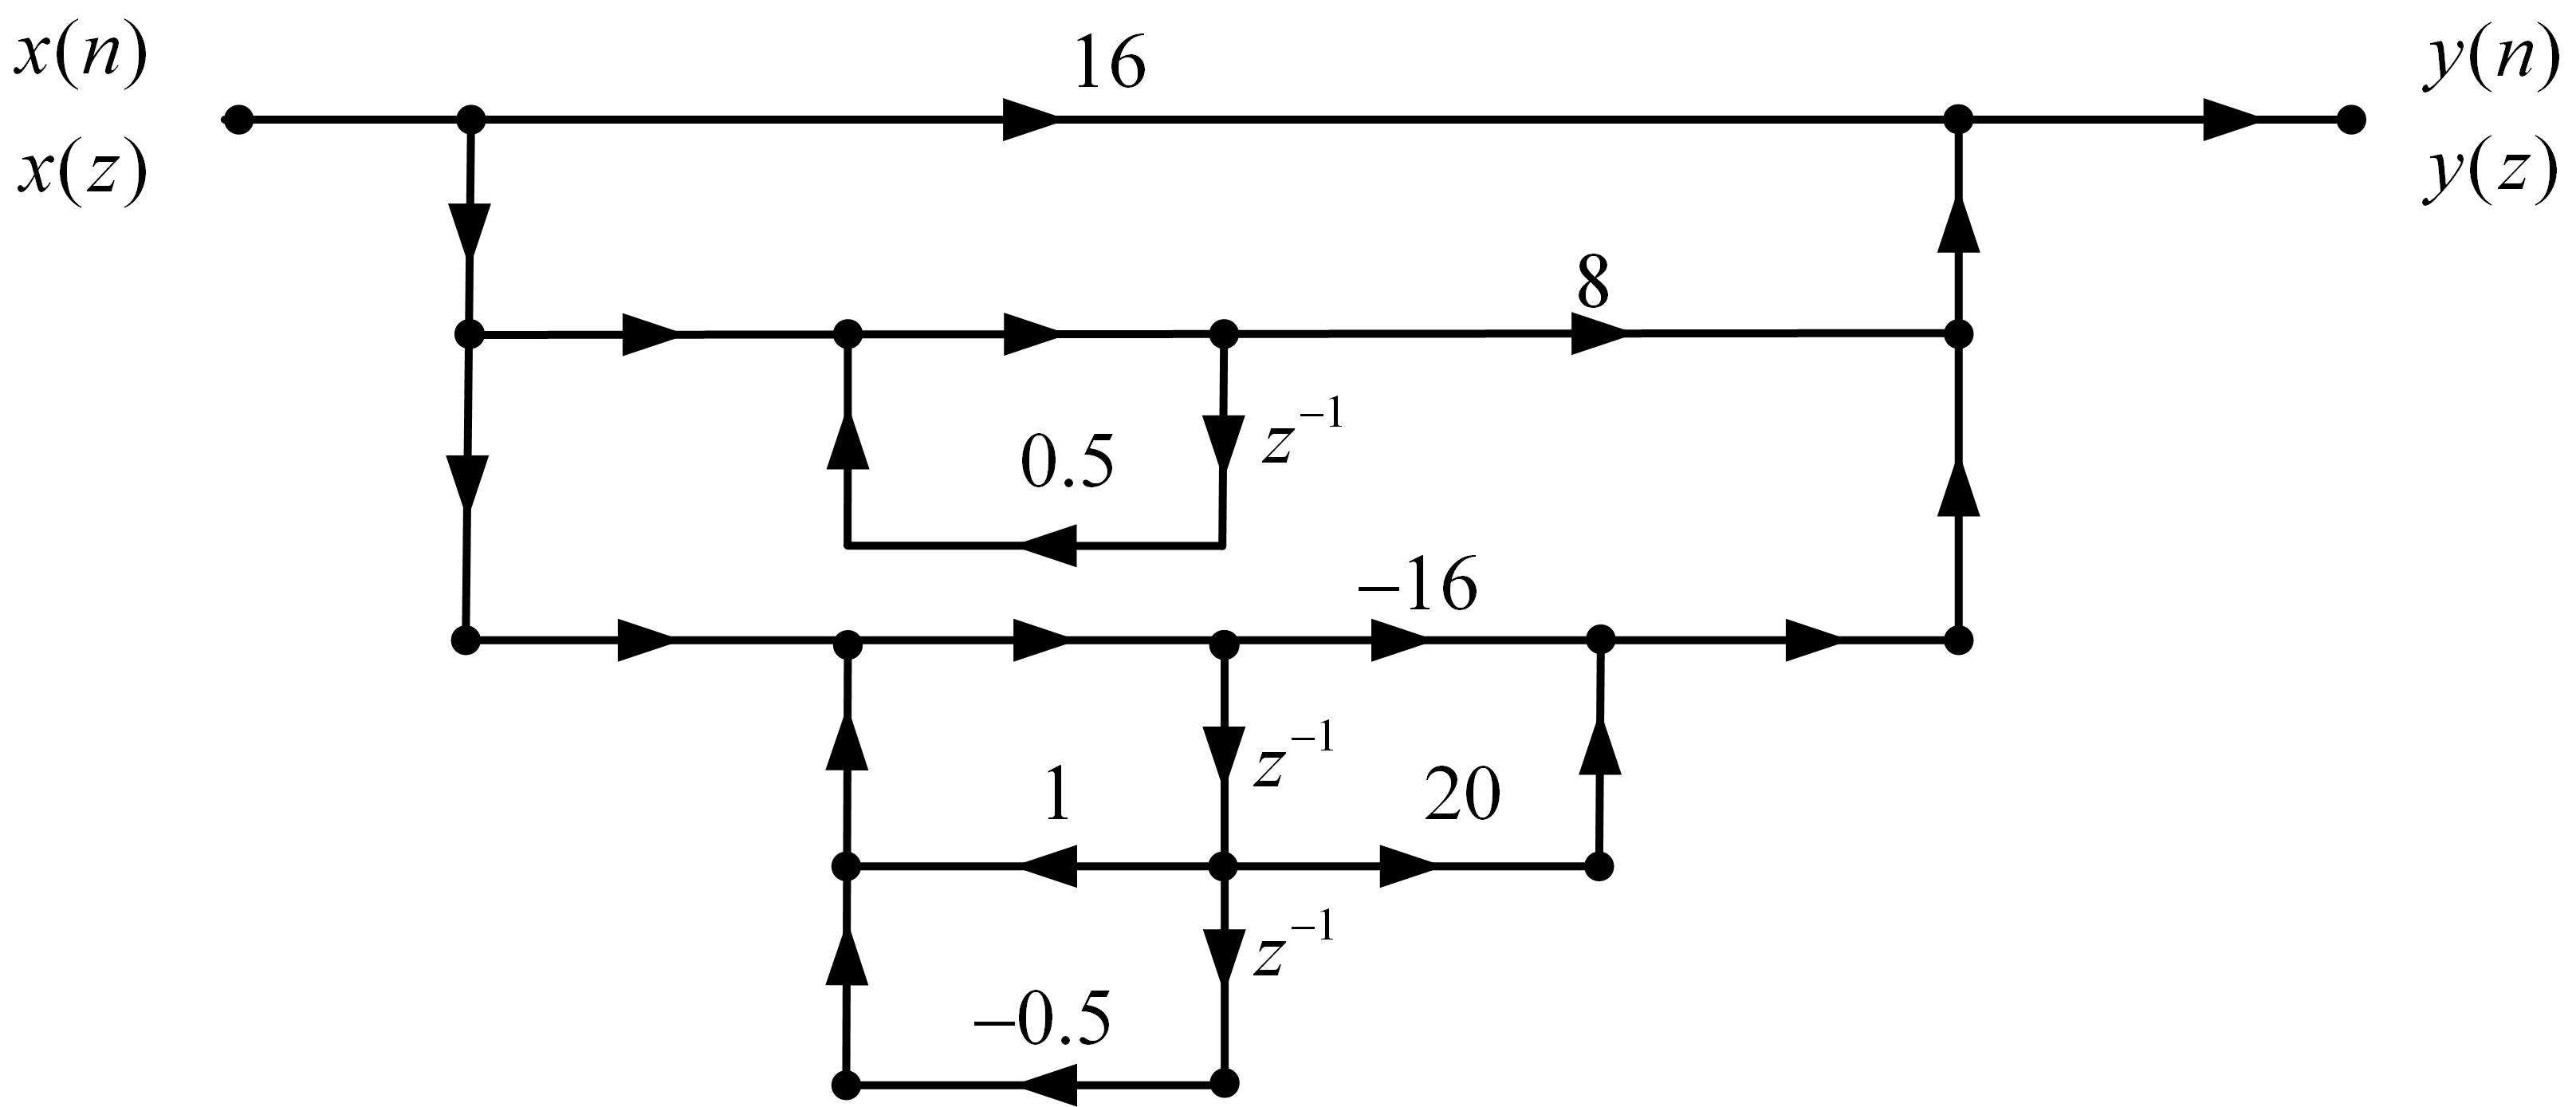
\includegraphics[width=0.85\textwidth]{binglianxingli.jpg}
\caption{例题的并联型结构示意图}
\label{chp5:jibenliutu}
\end{figure}
\end{frame}
%%%%%%%%%%%%%%%%%%%%%%%%%%%%%%%%%%%%%%%%%%%%%%%%%%%%%%%%%%%%%%%%%%%%%%%%%%%%%%%%%%%%%%%%%%%%%%%%%%%%%%%%%%%%%%%%%%%%%%%%%%%%%%%%%%%%
%%%%%
%%%%%
%%%%%%%%%%%%%%%%%%%%%%%%%%%%%%%%%%%%%%%%%%%%%%%%%%%%%%%%%%%%%%%%%%%%%%%%%%%%%%%%%%%%%%%%%%%%%%%%%%%%%%%%%%%%%%%%%%%%%%%%%%%%%%%%%%%%
\section{5.4 FIR系统的基本网络结构}
%%%%%%%%%%%%%%%%%%%%%%%%%%%%%%%%%%%%%%%%%%%%%%%%%%%%%%%%%%%%%%%%%%%%%%%%%%%%%%%%%%%%%%%%%%%%%%%%%%%%%%%%%%%%%%%%%%%%%%%%%%%%%%%%%%%%
%%%%%
%%%%%
%%%%%%%%%%%%%%%%%%%%%%%%%%%%%%%%%%%%%%%%%%%%%%%%%%%%%%%%%%%%%%%%%%%%%%%%%%%%%%%%%%%%%%%%%%%%%%%%%%%%%%%%%%%%%%%%%%%%%%%%%%%%%%%%%%%%
\begin{frame}\frametitle{FIR系统的基本网络结构的特点}%[allowframebreaks]

FIR网络结构特点是:\par

\textbf{没有反馈支路,即没有环路。}所以,其单位脉冲响应$h(n)$必定是有限长。
\newline

设其长度为N,则其系统函数为:
$$H(z) = \sum_{n=0}^{N-1}h(n)z^{-n}=\sum_{n=n_1}^{n_2}h(n)z^{-n}$$
%\par 可见$H(z)$是$z^{-1}$为自变量的N-1阶多项式。
%\par 即:
%$$H(z)=\frac{a_0z^{N-1}+a_1z^{N-2}+\cdots+a_{N-1}}{z^{N-1}}\quad\quad
%\quad\quad\quad\quad\quad\quad$$
%\par $\therefore\quad$$z=0$是$H(z)$的$N-1$阶极点。
第二章曾经指出,有限长序列的z变换,当$n_1\geq0,n_2>0$时,其收敛域为$0<|z|\leq\infty$。
可见其收敛域必然包括单位圆。
\newline
\pause
\begin{dablock}
 FIR-DF必定是稳定的,FIR-DF的设计不必考虑其稳定性。
\end{dablock}
\end{frame}
%%%%%%%%%%%%%%%%%%%%%%%%%%%%%%%%%%%%%%%%%%%%%%%%%%%%%%%%%%%%%%%%%%%%%%%%%%%%%%%%%%%%%%%%%%%%%%%%%%%%%%%%%%%%%%%%%%%%%%%%%%%%%%%%%%%%
%%%%%
%%%%%
%%%%%%%%%%%%%%%%%%%%%%%%%%%%%%%%%%%%%%%%%%%%%%%%%%%%%%%%%%%%%%%%%%%%%%%%%%%%%%%%%%%%%%%%%%%%%%%%%%%%%%%%%%%%%%%%%%%%%%%%%%%%%%%%%%%%
\subsection{5.4.1 直接型网络结构(卷积型)}
%%%%%%%%%%%%%%%%%%%%%%%%%%%%%%%%%%%%%%%%%%%%%%%%%%%%%%%%%%%%%%%%%%%%%%%%%%%%%%%%%%%%%%%%%%%%%%%%%%%%%%%%%%%%%%%%%%%%%%%%%%%%%%%%%%%%
%%%%%
%%%%%
%%%%%%%%%%%%%%%%%%%%%%%%%%%%%%%%%%%%%%%%%%%%%%%%%%%%%%%%%%%%%%%%%%%%%%%%%%%%%%%%%%%%%%%%%%%%%%%%%%%%%%%%%%%%%%%%%%%%%%%%%%%%%%%%%%%%
\begin{frame}\frametitle{直接型网络结构(卷积型)}%[allowframebreaks]

FIR-DF的差分方程为:
\begin{equation*}
\begin{split}
y(n)  &=x(n)*h(n)=\sum_{m=0}^{N-1}h(m)x(n-m)\\
     &= h(0)x(n) + h(1)x(n-1) +\cdots + H(N-1)x(n-(N-1))\\
\end{split}
\end{equation*}
其网络结构如下图所示:
\begin{figure}[h]
\centering
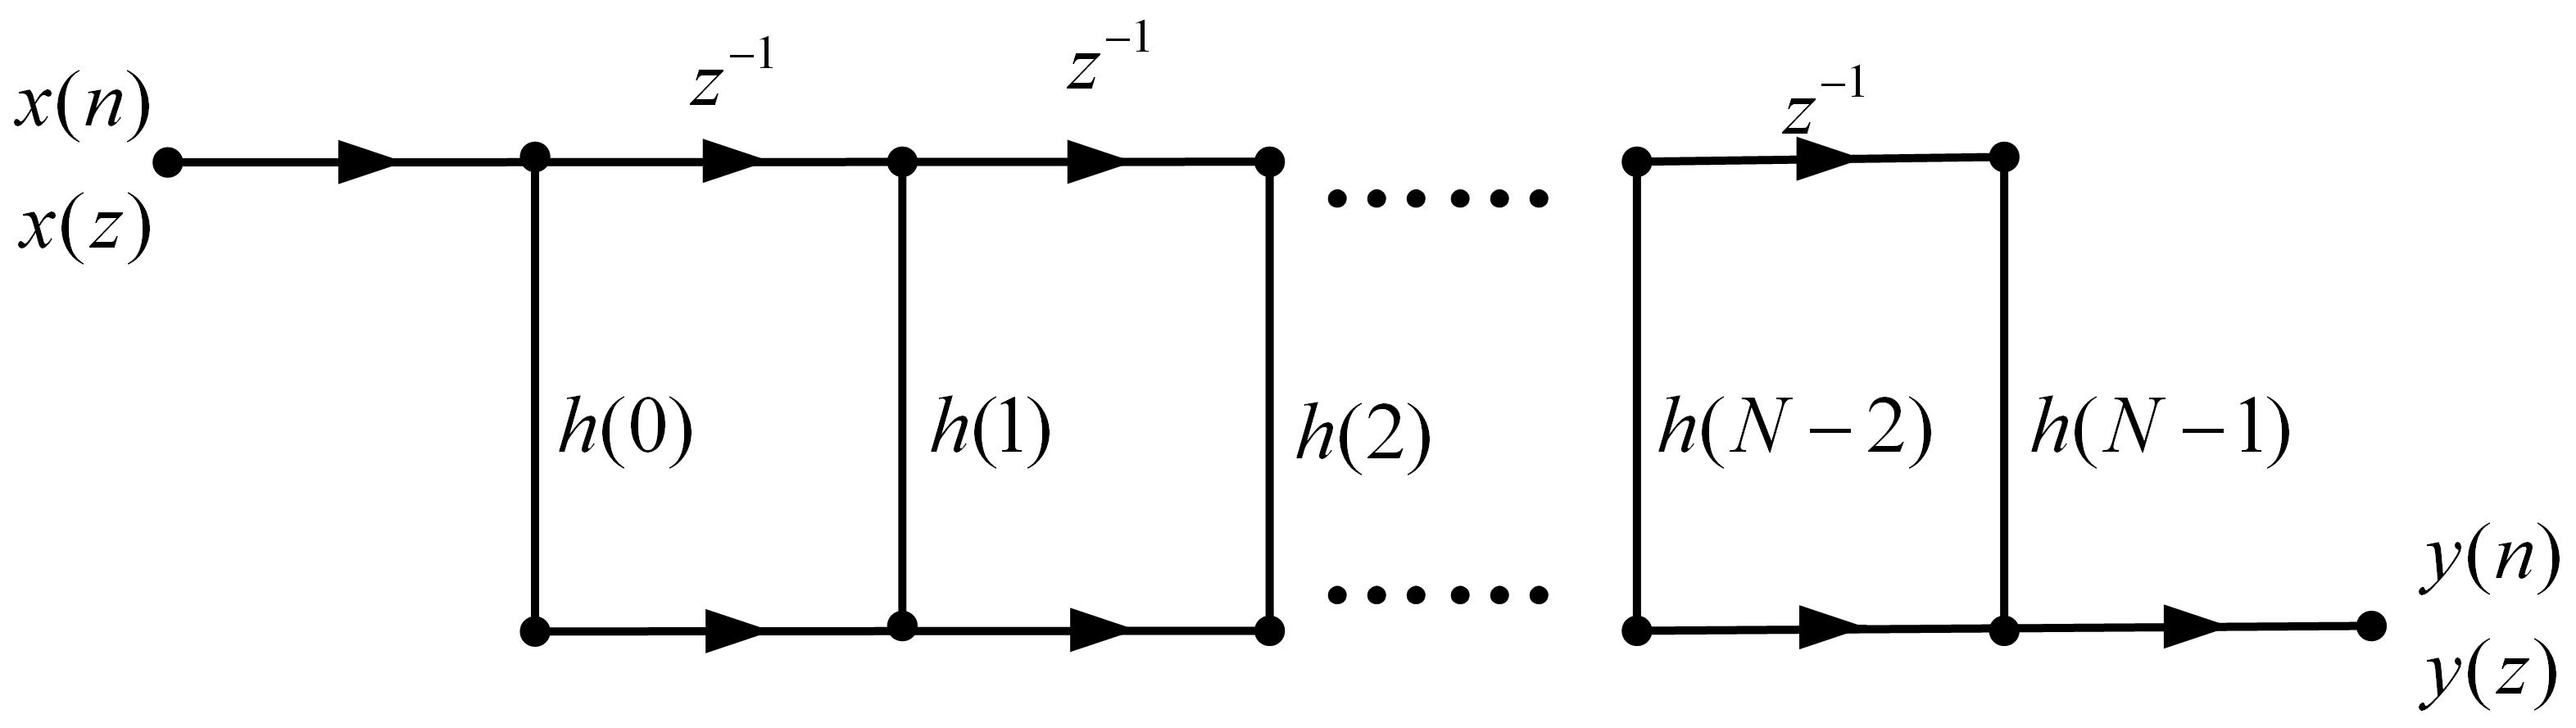
\includegraphics[width=0.9\textwidth]{firzhijie.jpg}
%\caption{直接型(卷积型)网络结构}
%\label{chp5:jibenliutu}
\end{figure}
\end{frame}
%%%%%%%%%%%%%%%%%%%%%%%%%%%%%%%%%%%%%%%%%%%%%%%%%%%%%%%%%%%%%%%%%%%%%%%%%%%%%%%%%%%%%%%%%%%%%%%%%%%%%%%%%%%%%%%%%%%%%%%%%%%%%%%%%%%%
%%%%%
%%%%%
%%%%%%%%%%%%%%%%%%%%%%%%%%%%%%%%%%%%%%%%%%%%%%%%%%%%%%%%%%%%%%%%%%%%%%%%%%%%%%%%%%%%%%%%%%%%%%%%%%%%%%%%%%%%%%%%%%%%%%%%%%%%%%%%%%%%
\begin{frame}\frametitle{直接型网络结构(卷积型)}%[allowframebreaks]
\par 也可通过其系统函数理解,FIR-DF的系统函数为:
\begin{equation*}
\begin{split}
H(z) &=\sum_{n=0}^{N-1}h(n)z^{-n}\\
     &= h(0) + h(1)z^{-1} + h(2)z^{-2} +\cdots + H(N-1)z^{-(N-1)}\\
\end{split}
\end{equation*}
\par 同样可以画出流图。
\begin{figure}[h]
\centering
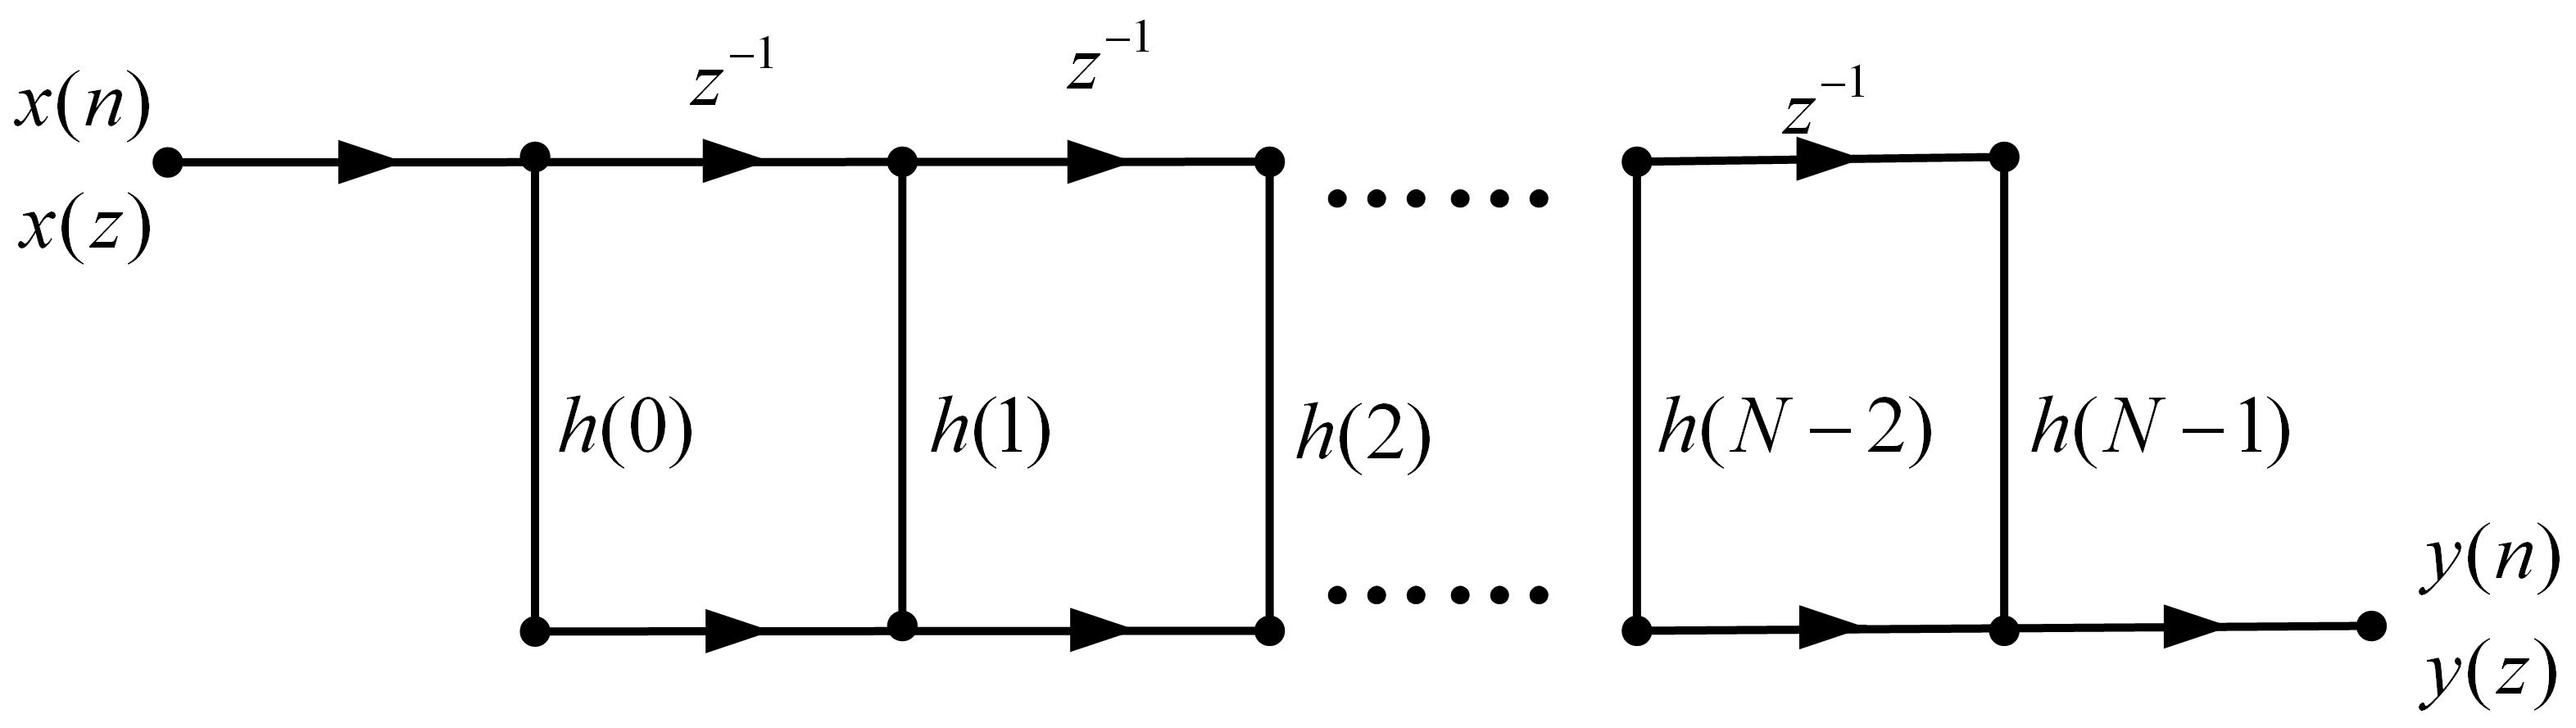
\includegraphics[width=0.9\textwidth]{firzhijie.jpg}
%\caption{直接型(卷积型)网络结构}
%\label{chp5:jibenliutu}
\end{figure}
\end{frame}
%%%%%%%%%%%%%%%%%%%%%%%%%%%%%%%%%%%%%%%%%%%%%%%%%%%%%%%%%%%%%%%%%%%%%%%%%%%%%%%%%%%%%%%%%%%%%%%%%%%%%%%%%%%%%%%%%%%%%%%%%%%%%%%%%%%%
%%%%%
%%%%%
%%%%%%%%%%%%%%%%%%%%%%%%%%%%%%%%%%%%%%%%%%%%%%%%%%%%%%%%%%%%%%%%%%%%%%%%%%%%%%%%%%%%%%%%%%%%%%%%%%%%%%%%%%%%%%%%%%%%%%%%%%%%%%%%%%%%
\subsection{5.4.2 级联型网络结构(串联型)}
%%%%%%%%%%%%%%%%%%%%%%%%%%%%%%%%%%%%%%%%%%%%%%%%%%%%%%%%%%%%%%%%%%%%%%%%%%%%%%%%%%%%%%%%%%%%%%%%%%%%%%%%%%%%%%%%%%%%%%%%%%%%%%%%%%%%
%%%%%
%%%%%
%%%%%%%%%%%%%%%%%%%%%%%%%%%%%%%%%%%%%%%%%%%%%%%%%%%%%%%%%%%%%%%%%%%%%%%%%%%%%%%%%%%%%%%%%%%%%%%%%%%%%%%%%%%%%%%%%%%%%%%%%%%%%%%%%%%%
\begin{frame}\frametitle{级联型网络结构(串联型)}%[allowframebreaks]
将系统函数$H(z)$因式分解为一阶或二阶的因子,每一个因式都用直接型实现。
$$H(z)=H_1(z)\cdot H_2(z) \cdots H_k(z)$$
    \begin{example}
        \par 已知:$H(z) = 0.96+2z^{-1}+2.8z^{-2}+1.5z^{-3}$,画出其卷积型与级联型网络结构。
    \end{example}
%\newline\newline\newline\newline
\end{frame}
%%%%%%%%%%%%%%%%%%%%%%%%%%%%%%%%%%%%%%%%%%%%%%%%%%%%%%%%%%%%%%%%%%%%%%%%%%%%%%%%%%%%%%%%%%%%%%%%%%%%%%%%%%%%%%%%%%%%%%%%%%%%%%%%%%%%
%%%%%
%%%%%
%%%%%%%%%%%%%%%%%%%%%%%%%%%%%%%%%%%%%%%%%%%%%%%%%%%%%%%%%%%%%%%%%%%%%%%%%%%%%%%%%%%%%%%%%%%%%%%%%%%%%%%%%%%%%%%%%%%%%%%%%%%%%%%%%%%%
\begin{frame}\frametitle{(1)卷积型网络结构}%[allowframebreaks]
    \begin{example}
        \par 已知:$H(z) = 0.96+2z^{-1}+2.8z^{-2}+1.5z^{-3}$,画出其卷积型与级联型网络结构。
    \end{example}
    \begin{answer}
        卷积型网络结构为
        \begin{figure}[h]
            \centering
            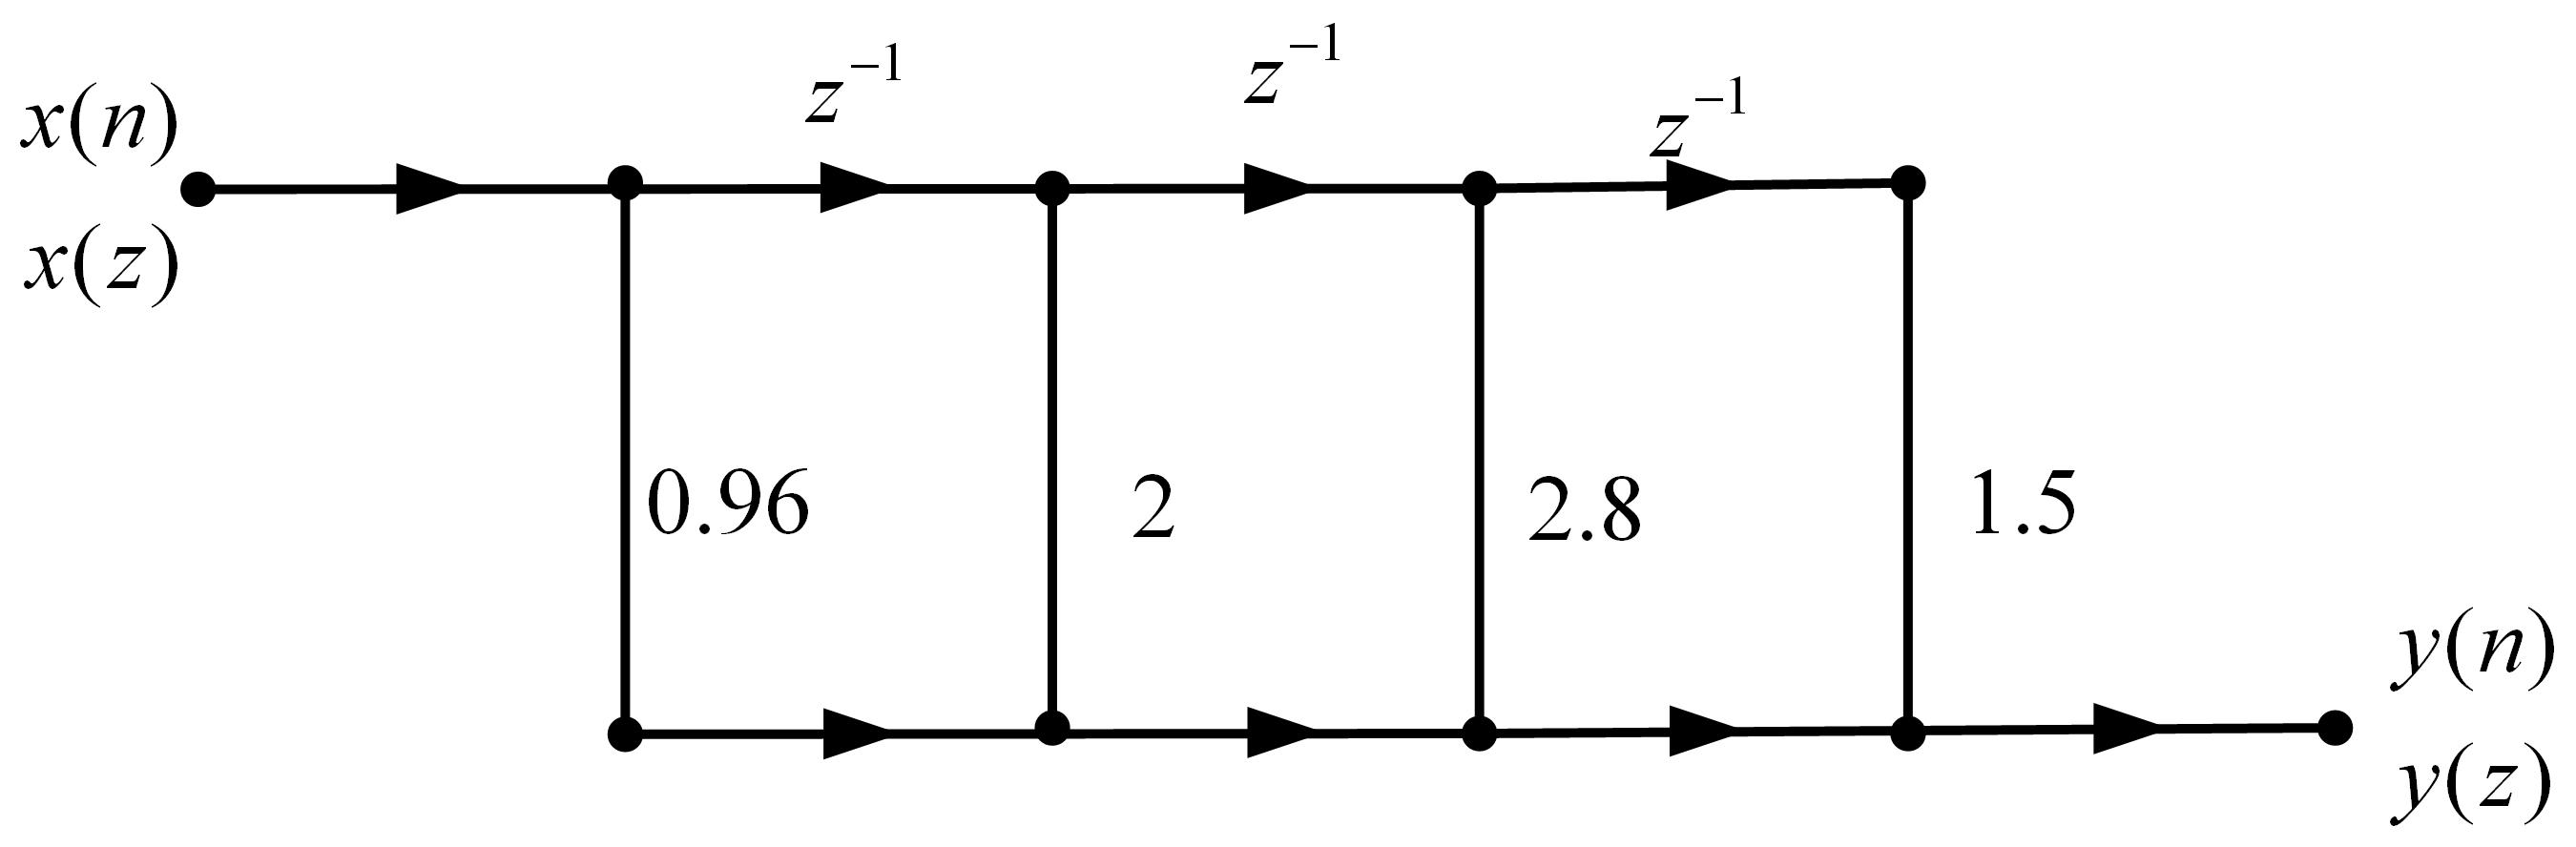
\includegraphics[width=0.6\textwidth]{lijuanjixing.jpg}
            %\caption{例题的卷积型网络结构}
            %\label{chp5:jibenliutu}
        \end{figure}
     \vspace{0.2cm}
    \end{answer}
\end{frame}
%%%%%%%%%%%%%%%%%%%%%%%%%%%%%%%%%%%%%%%%%%%%%%%%%%%%%%%%%%%%%%%%%%%%%%%%%%%%%%%%%%%%%%%%%%%%%%%%%%%%%%%%%%%%%%%%%%%%%%%%%%%%%%%%%%%%
%%%%%
%%%%%
%%%%%%%%%%%%%%%%%%%%%%%%%%%%%%%%%%%%%%%%%%%%%%%%%%%%%%%%%%%%%%%%%%%%%%%%%%%%%%%%%%%%%%%%%%%%%%%%%%%%%%%%%%%%%%%%%%%%%%%%%%%%%%%%%%%%
\begin{frame}[shrink]\frametitle{(2)级联型网络结构}%[allowframebreaks]
\begin{example}
已知:$H(z) = 0.96+2z^{-1}+2.8z^{-2}+1.5z^{-3}$,画出其卷积型与级联型网络结构。
\end{example}
\begin{answer}
因式分解可得:
$$H(z) = (0.6+0.5z^{-1})(1.6+2z^{-1}+3z^{-2})=H_1(z)\cdot H_2(z)$$
\begin{figure}[h]
\centering
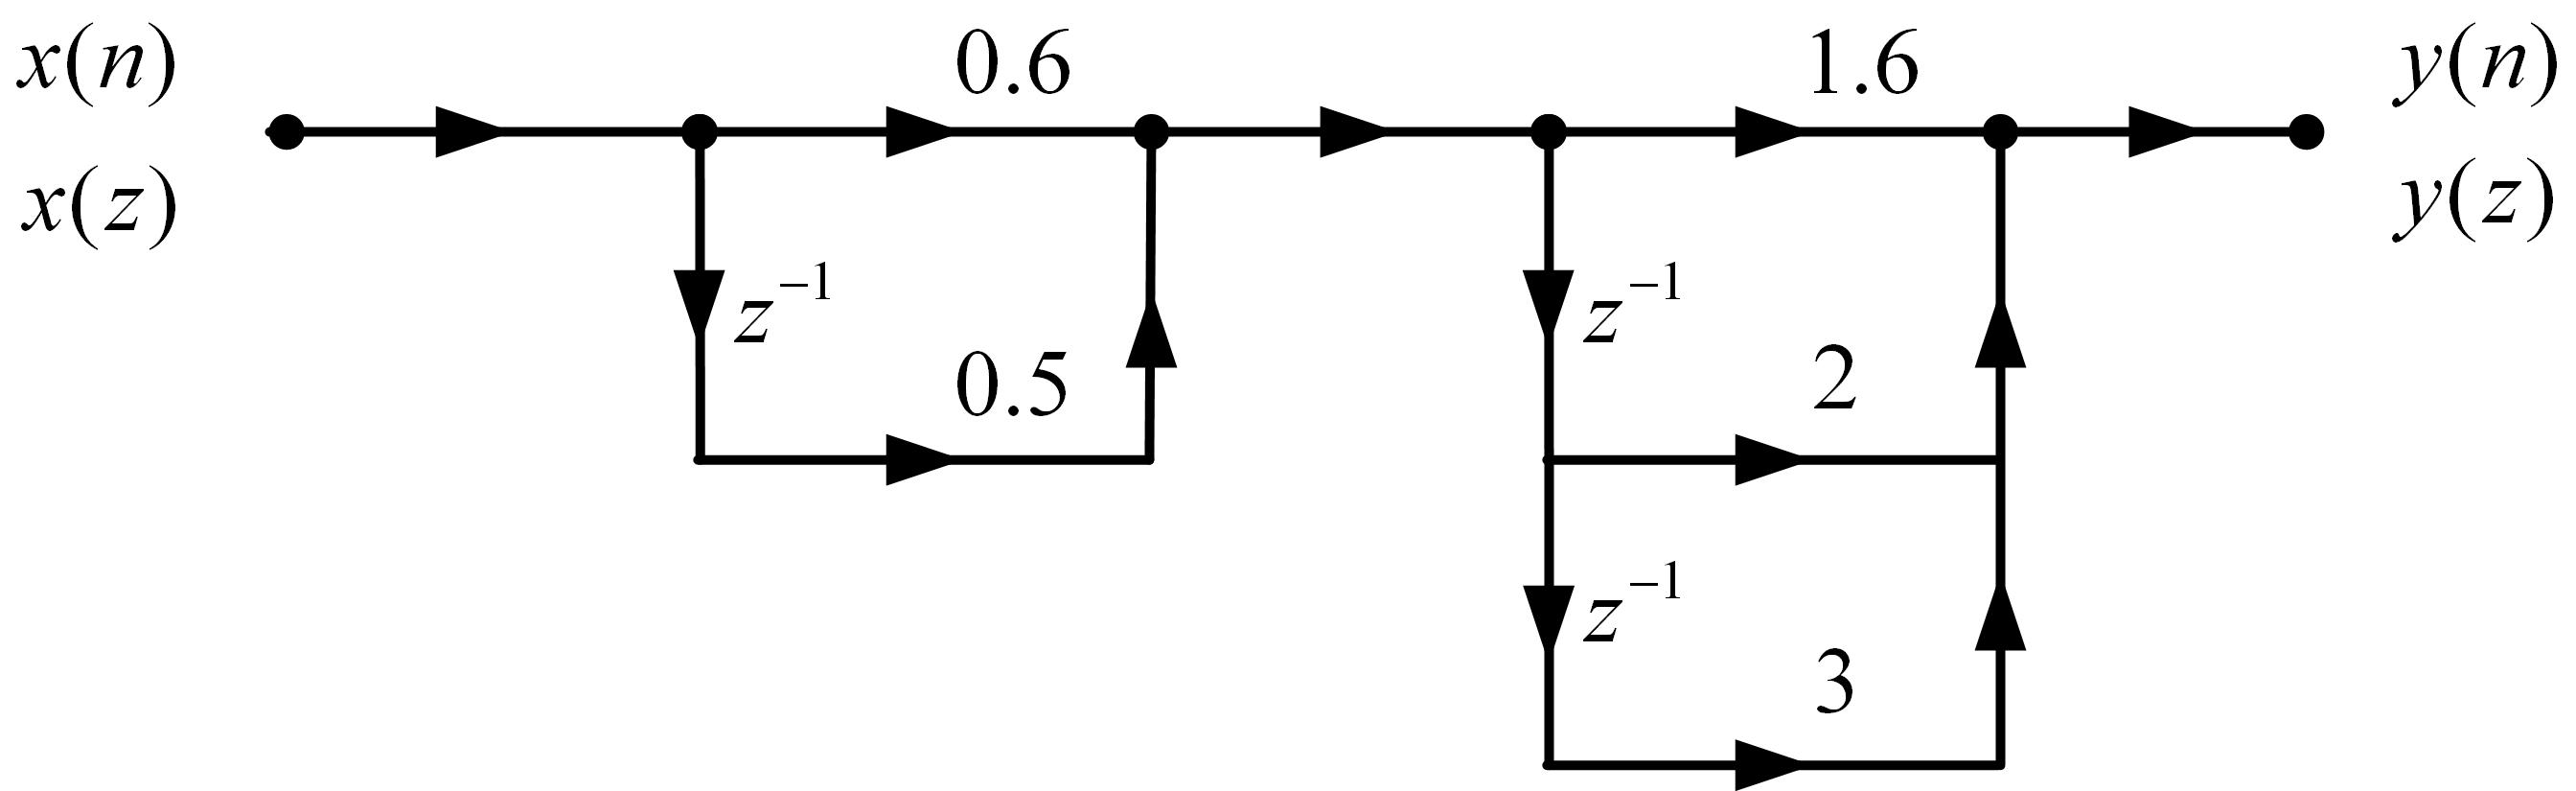
\includegraphics[width=0.7\textwidth]{lijilianxing.jpg}
%\caption{例题的级联网络结构}
%\label{chp5:jibenliutu}
\end{figure}
%\vspace{0.1cm}
\end{answer}
\end{frame}
%%%%%%%%%%%%%%%%%%%%%%%%%%%%%%%%%%%%%%%%%%%%%%%%%%%%%%%%%%%%%%%%%%%%%%%%%%%%%%%%%%%%%%%%%%%%%%%%%%%%%%%%%%%%%%%%%%%%%%%%%%%%%%%%%%%%
%%%%%
%%%%%
%%%%%%%%%%%%%%%%%%%%%%%%%%%%%%%%%%%%%%%%%%%%%%%%%%%%%%%%%%%%%%%%%%%%%%%%%%%%%%%%%%%%%%%%%%%%%%%%%%%%%%%%%%%%%%%%%%%%%%%%%%%%%%%%%%%%
\subsection{5.4.3 线性相位结构}
%%%%%%%%%%%%%%%%%%%%%%%%%%%%%%%%%%%%%%%%%%%%%%%%%%%%%%%%%%%%%%%%%%%%%%%%%%%%%%%%%%%%%%%%%%%%%%%%%%%%%%%%%%%%%%%%%%%%%%%%%%%%%%%%%%%%
%%%%%
%%%%%
%%%%%%%%%%%%%%%%%%%%%%%%%%%%%%%%%%%%%%%%%%%%%%%%%%%%%%%%%%%%%%%%%%%%%%%%%%%%%%%%%%%%%%%%%%%%%%%%%%%%%%%%%%%%%%%%%%%%%%%%%%%%%%%%%%%%
\begin{frame}\frametitle{线性相位结构}%[allowframebreaks]
\begin{enumerate}
  \item 线性相位结构是FIR系统的直接型结构的简化,特点是网络具有线性相位特性,
比直接型结构节约了近一半的乘法器。
  \item FIR-DF的频率响应特性较易于设计为线性相位结构。
\end{enumerate}



\end{frame}
%%%%%%%%%%%%%%%%%%%%%%%%%%%%%%%%%%%%%%%%%%%%%%%%%%%%%%%%%%%%%%%%%%%%%%%%%%%%%%%%%%%%%%%%%%%%%%%%%%%%%%%%%%%%%%%%%%%%%%%%%%%%%%%%%%%%
%%%%%
%%%%%
%%%%%%%%%%%%%%%%%%%%%%%%%%%%%%%%%%%%%%%%%%%%%%%%%%%%%%%%%%%%%%%%%%%%%%%%%%%%%%%%%%%%%%%%%%%%%%%%%%%%%%%%%%%%%%%%%%%%%%%%%%%%%%%%%%%%
\subsubsection{线性相位结构的概念}
%%%%%%%%%%%%%%%%%%%%%%%%%%%%%%%%%%%%%%%%%%%%%%%%%%%%%%%%%%%%%%%%%%%%%%%%%%%%%%%%%%%%%%%%%%%%%%%%%%%%%%%%%%%%%%%%%%%%%%%%%%%%%%%%%%%%
%%%%%
%%%%%
%%%%%%%%%%%%%%%%%%%%%%%%%%%%%%%%%%%%%%%%%%%%%%%%%%%%%%%%%%%%%%%%%%%%%%%%%%%%%%%%%%%%%%%%%%%%%%%%%%%%%%%%%%%%%%%%%%%%%%%%%%%%%%%%%%%%
\begin{frame}\frametitle{线性相位结构的概念}%[allowframebreaks]
%\textbf{一、线性相位结构的概念}


我们知道,一个滤波器的描述方式有三种:
$$\underbrace{h(n)}_{\mbox{单位脉冲响应}}\Longleftrightarrow \underbrace{H(z)}_{\mbox{系统函数}}\Longleftrightarrow \underbrace{H(e^{j\omega})}_{\mbox{频率响应函数}}$$
且有:
$$H(e^{j\omega})=H(z)|_{z=e^{j\omega}}$$
同时有:
%$$H(e^{j\omega})=\underbrace{|H(e^{j\omega})|}_{\mbox{幅频特性函数}}\cdot \underbrace{e^{j\varphi(\omega)}}_{\mbox{相频特性函数}}$$
$$H(e^{j\omega})= |H(e^{j\omega})|\cdot e^{j\varphi(\omega)}$$

\par $|H(e^{j\omega})|$称为幅频特性函数。
\par $\varphi(\omega)$称为相频特性函数。
\par \textbf{所谓线性相位,就是指$\varphi(\omega)$是$\omega$的线性函数。}
\end{frame}
%%%%%%%%%%%%%%%%%%%%%%%%%%%%%%%%%%%%%%%%%%%%%%%%%%%%%%%%%%%%%%%%%%%%%%%%%%%%%%%%%%%%%%%%%%%%%%%%%%%%%%%%%%%%%%%%%%%%%%%%%%%%%%%%%%%%
%%%%%
%%%%%
%%%%%%%%%%%%%%%%%%%%%%%%%%%%%%%%%%%%%%%%%%%%%%%%%%%%%%%%%%%%%%%%%%%%%%%%%%%%%%%%%%%%%%%%%%%%%%%%%%%%%%%%%%%%%%%%%%%%%%%%%%%%%%%%%%%%
\subsubsection{FIR-DF的线性相位结构}
%%%%%%%%%%%%%%%%%%%%%%%%%%%%%%%%%%%%%%%%%%%%%%%%%%%%%%%%%%%%%%%%%%%%%%%%%%%%%%%%%%%%%%%%%%%%%%%%%%%%%%%%%%%%%%%%%%%%%%%%%%%%%%%%%%%%
%%%%%
%%%%%
%%%%%%%%%%%%%%%%%%%%%%%%%%%%%%%%%%%%%%%%%%%%%%%%%%%%%%%%%%%%%%%%%%%%%%%%%%%%%%%%%%%%%%%%%%%%%%%%%%%%%%%%%%%%%%%%%%%%%%%%%%%%%%%%%%%%
\begin{frame}\frametitle{线性相位结构FIR-DF的单位脉冲响应$h(n)$的特点}%[allowframebreaks]
可以证明,如果一个FIR-DF具有线性相位结构,其单位脉冲响应$h(n)$应满足下面公式:
$$h(n)=\pm h(N-1-n)$$
式中
\par “+”代表第一类线性相位结构,
\par “-”代表第二类线性相位结构。
\end{frame}
%%%%%%%%%%%%%%%%%%%%%%%%%%%%%%%%%%%%%%%%%%%%%%%%%%%%%%%%%%%%%%%%%%%%%%%%%%%%%%%%%%%%%%%%%%%%%%%%%%%%%%%%%%%%%%%%%%%%%%%%%%%%%%%%%%%%
%%%%%
%%%%%
%%%%%%%%%%%%%%%%%%%%%%%%%%%%%%%%%%%%%%%%%%%%%%%%%%%%%%%%%%%%%%%%%%%%%%%%%%%%%%%%%%%%%%%%%%%%%%%%%%%%%%%%%%%%%%%%%%%%%%%%%%%%%%%%%%%%
\begin{frame}\frametitle{(1)设N为偶数,且$h(n)= h(N-1-n)$}%[allowframebreaks]
%设N为偶数,且$h(n)= h(N-1-n)$
    \begin{equation*}
        \begin{split}
        H(z) &= \sum_{n=0}^{N-1}h(n)z^{-n}\\
             &= \sum_{n=0}^{\frac{N}{2}-1}h(n)z^{-n}+ \sum_{n=\frac{N}{2}}^{N-1}h(n)z^{-n}\\
             &= \sum_{n=0}^{\frac{N}{2}-1}h(n)z^{-n}+\underbrace{
                \sum_{m=0}^{\frac{N}{2}-1}h(N-1-m)z^{-(N-1-m)}}_{\mbox{令$m=N-1-n$}}\\
%             &= \sum_{n=0}^{\frac{N}{2}-1}h(n)z^{-n}+\underbrace{
%                \sum_{n=0}^{\frac{N}{2}-1}h(N-1-n)z^{-(N-1-n)}}_{\mbox{将m换为n}} \\    %\newpage
%             &= \sum_{n=0}^{\frac{N}{2}-1}h(n)z^{-n}+\sum_{n=0}^{\frac{N}{2}-1}h(n)z^{-(N-1-n)}\\
%             &= \sum_{n=0}^{\frac{N}{2}-1}h(n)\left[ z^{-n}+z^{-(N-1-n)}\right]
        \end{split}
    \end{equation*}
    %可见,乘法次数减半,结构更优化。
\end{frame}
%%%%%%%%%%%%%%%%%%%%%%%%%%%%%%%%%%%%%%%%%%%%%%%%%%%%%%%%%%%%%%%%%%%%%%%%%%%%%%%%%%%%%%%%%%%%%%%%%%%%%%%%%%%%%%%%%%%%%%%%%%%%%%%%%%%%
%%%%%
%%%%%
%%%%%%%%%%%%%%%%%%%%%%%%%%%%%%%%%%%%%%%%%%%%%%%%%%%%%%%%%%%%%%%%%%%%%%%%%%%%%%%%%%%%%%%%%%%%%%%%%%%%%%%%%%%%%%%%%%%%%%%%%%%%%%%%%%%%
\begin{frame}[shrink]\frametitle{(1)设N为偶数,且$h(n)= h(N-1-n)$}%[allowframebreaks]
%设N为偶数,且$h(n)= h(N-1-n)$
    \begin{equation*}
        \begin{split}
%        H(z) &= \sum_{n=0}^{N-1}h(n)z^{-n}\\
%             &= \sum_{n=0}^{\frac{N}{2}-1}h(n)z^{-n}+\underbrace{
%                \sum_{n=\frac{N}{2}}^{N-1}h(n)z^{-n}}_{\mbox{令$m=N-1-n$}}\\
        H(z)  &= \sum_{n=0}^{\frac{N}{2}-1}h(n)z^{-n}+\underbrace{\sum_{n=0}^{\frac{N}{2}-1}h(N-1-n)z^{-(N-1-n)}}_{\mbox{将m换为n之后}} \\    %\newpage
%              &= \sum_{n=0}^{\frac{N}{2}-1}h(n)z^{-n}+\sum_{n=0}^{\frac{N}{2}-1}h(N-1-n)z^{-(N-1-n)} \\    %\newpage
              &= \sum_{n=0}^{\frac{N}{2}-1}h(n)z^{-n}+\sum_{n=0}^{\frac{N}{2}-1}h(n)z^{-(N-1-n)}\\
              &= \sum_{n=0}^{\frac{N}{2}-1}h(n)\left[ z^{-n}+z^{-(N-1-n)}\right]
        \end{split}
    \end{equation*}
    \par 可见,乘法次数减半,结构更优化。
\end{frame}
%%%%%%%%%%%%%%%%%%%%%%%%%%%%%%%%%%%%%%%%%%%%%%%%%%%%%%%%%%%%%%%%%%%%%%%%%%%%%%%%%%%%%%%%%%%%%%%%%%%%%%%%%%%%%%%%%%%%%%%%%%%%%%%%%%%%
%%%%%
%%%%%
%%%%%%%%%%%%%%%%%%%%%%%%%%%%%%%%%%%%%%%%%%%%%%%%%%%%%%%%%%%%%%%%%%%%%%%%%%%%%%%%%%%%%%%%%%%%%%%%%%%%%%%%%%%%%%%%%%%%%%%%%%%%%%%%%%%%
\begin{frame}[shrink]\frametitle{}%[allowframebreaks]
%\begin{example}
    例如,当N=8,则
%$H(z) = \sum_{n=0}^{3}h(n)\left[ z^{-n}+z^{-(7-n)}\right]$
%$$H(z) = h(0)(z^0+z^{-7})+h(1)(z^{-1}+z^{-6})+h(2)(z^{-2}+z^{-5})+h(3)(z^{-3}+z^{-4})$$
\begin{equation*} \label{eq:1}
\begin{split}
H(z) &= \sum_{n=0}^{3}h(n)\left[ z^{-n}+z^{-(7-n)}\right] \\
     &= h(0)(z^0+z^{-7})+h(1)(z^{-1}+z^{-6})+h(2)(z^{-2}+z^{-5}) \\
     &\quad +h(3)(z^{-3}+z^{-4})
\end{split}
\end{equation*}

%\end{example}
    \begin{figure}[h]
        \centering
        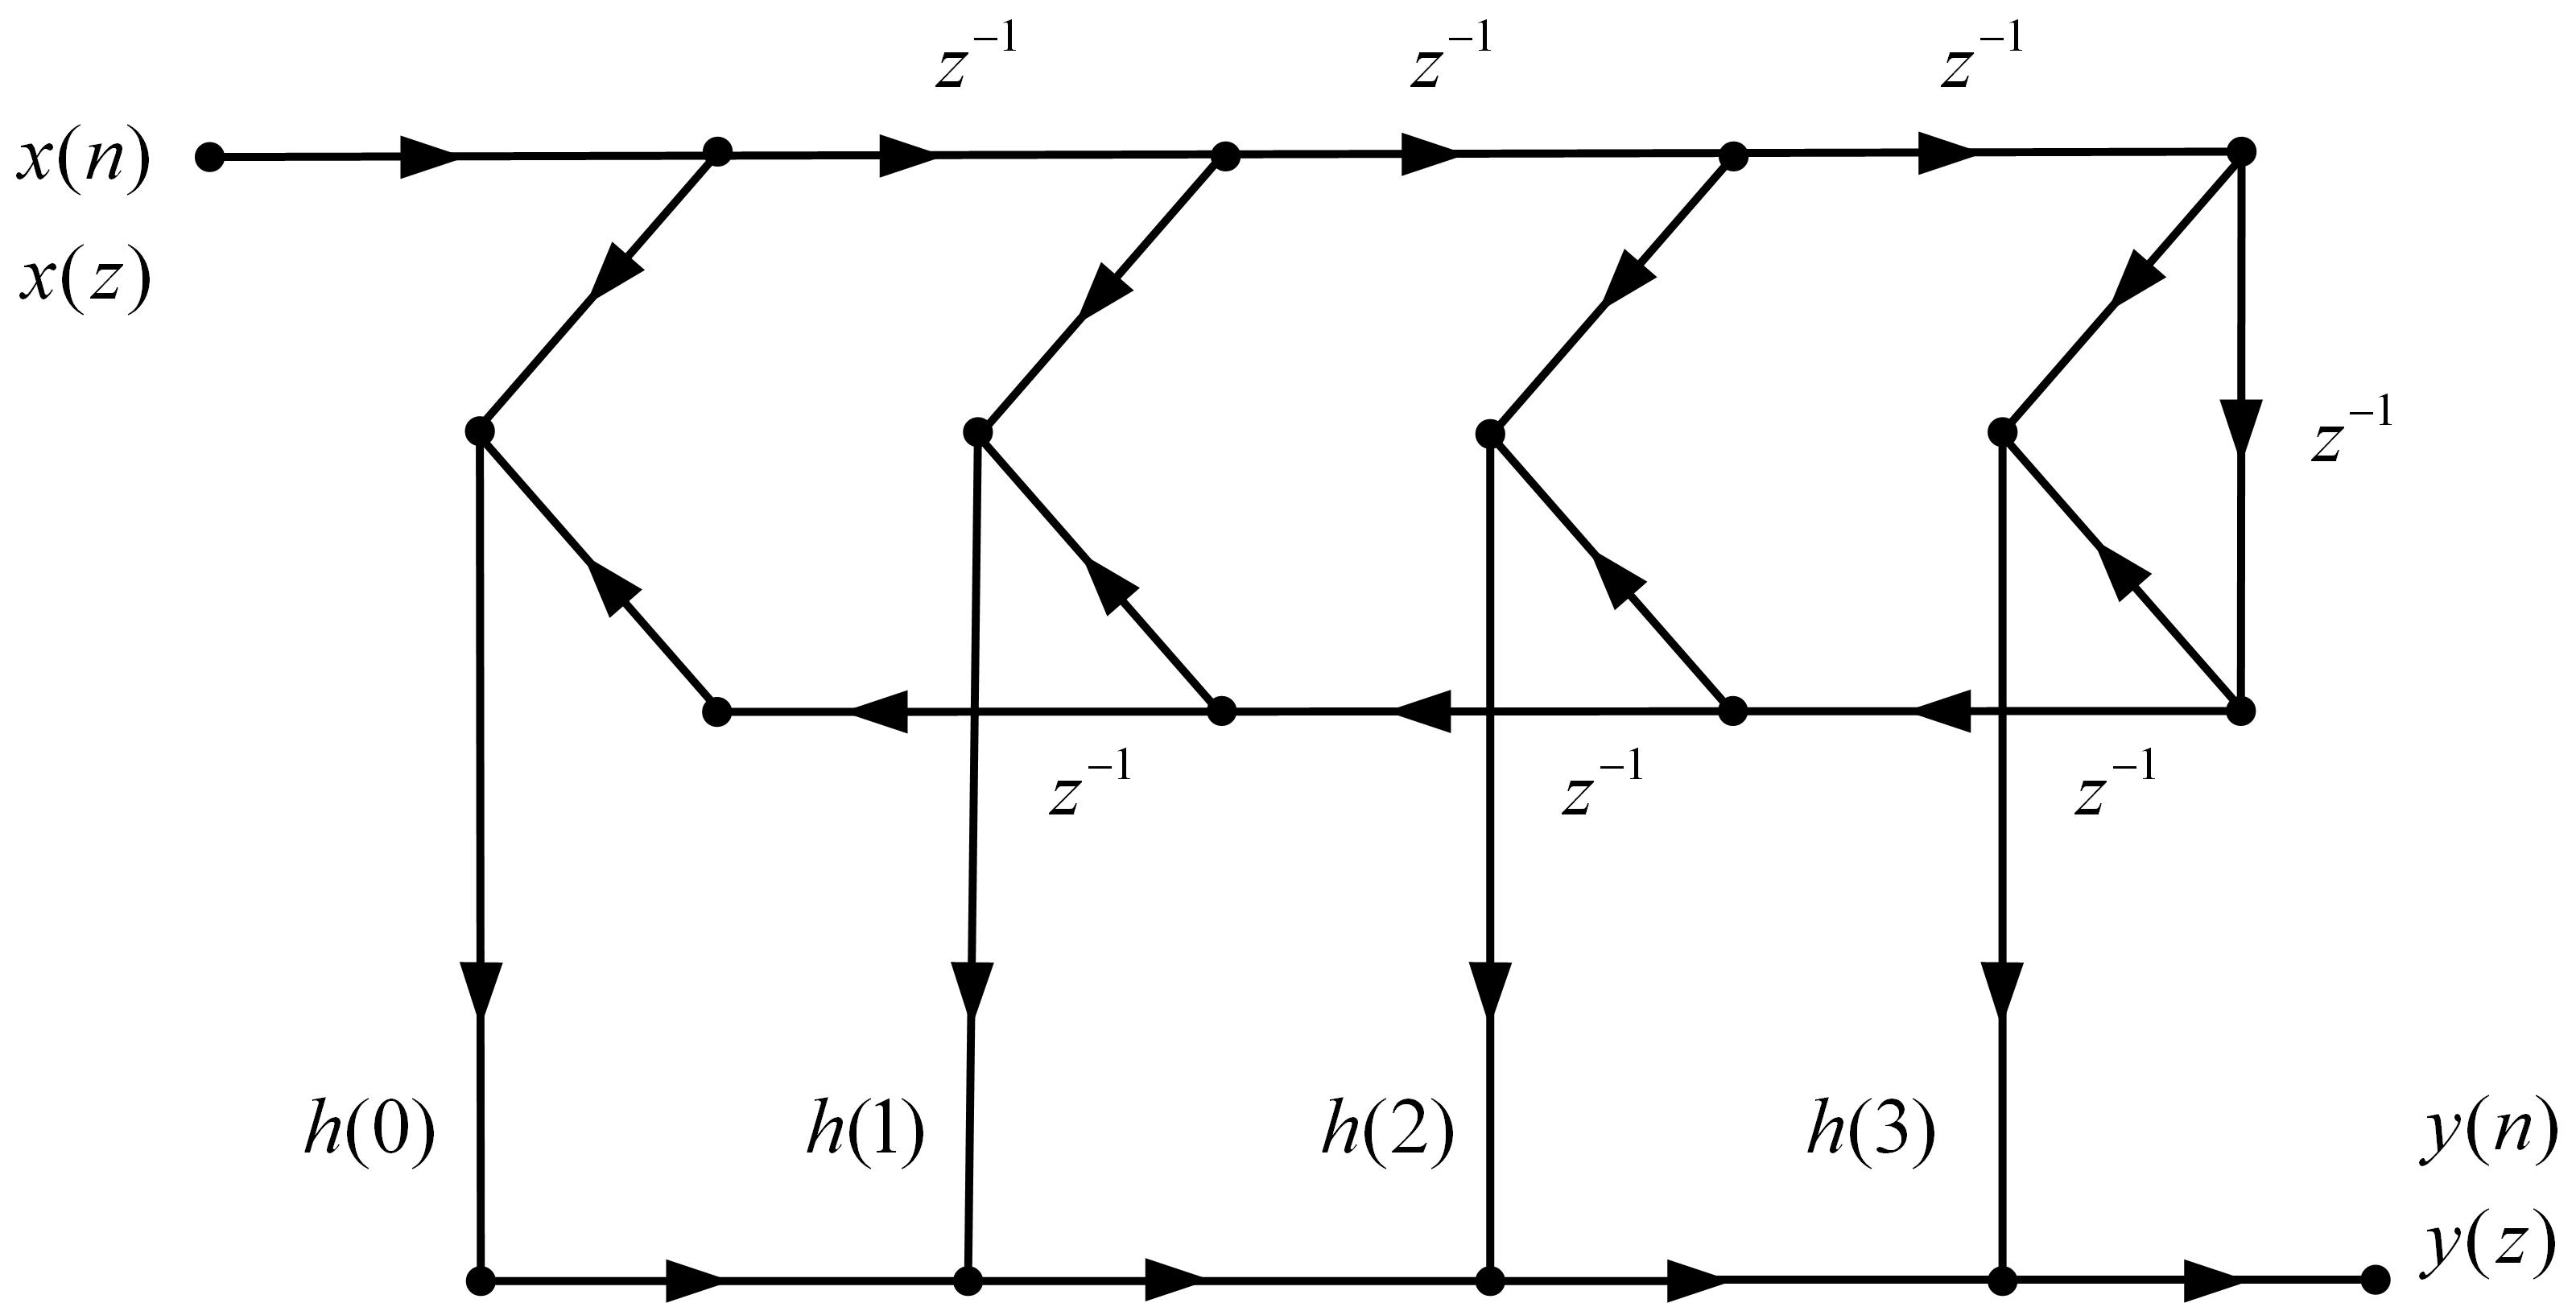
\includegraphics[width=0.75\textwidth]{osxxxw.jpg}
        %\caption{例题的第一类线性相位网络结构流图}
        %\label{chp5:jibenliutu}
    \end{figure}
\end{frame}
%%%%%%%%%%%%%%%%%%%%%%%%%%%%%%%%%%%%%%%%%%%%%%%%%%%%%%%%%%%%%%%%%%%%%%%%%%%%%%%%%%%%%%%%%%%%%%%%%%%%%%%%%%%%%%%%%%%%%%%%%%%%%%%%%%%%
%%%%%
%%%%%
%%%%%%%%%%%%%%%%%%%%%%%%%%%%%%%%%%%%%%%%%%%%%%%%%%%%%%%%%%%%%%%%%%%%%%%%%%%%%%%%%%%%%%%%%%%%%%%%%%%%%%%%%%%%%%%%%%%%%%%%%%%%%%%%%%%%
\begin{frame}\frametitle{(2)当N为偶数,且$h(n)= -h(N-1-n)$}%[allowframebreaks]
显然有:
    $$H(z) =\sum_{n=0}^{\frac{N}{2}-1}h(n)\left[ z^{-n}-z^{-(N-1-n)}\right]$$

\end{frame}
%%%%%%%%%%%%%%%%%%%%%%%%%%%%%%%%%%%%%%%%%%%%%%%%%%%%%%%%%%%%%%%%%%%%%%%%%%%%%%%%%%%%%%%%%%%%%%
\begin{frame}\frametitle{(3)当N为奇数,且$h(n)= h(N-1-n)$}%[allowframebreaks]
%当N为奇数,且$h(n)= h(N-1-n)$
\begin{equation*} \label{eq:1}
\begin{split}
H(z) &= \sum_{n=0}^{N-1}h(n)z^{-n}\\
&= \sum_{n=0}^{\frac{N-1}{2}-1}h(n)z^{-n}+ h(\frac{N-1}{2})z^{-\frac{N-1}{2}}+
\sum_{n=\frac{N-1}{2}+1}^{N-1}h(n)z^{-n}\\
&= \sum_{n=0}^{\frac{N-1}{2}-1}h(n)\left[ z^{-n}+z^{-(N-1-n)}\right]+h(\frac{N-1}{2})z^{-\frac{N-1}{2}}
\end{split}
\end{equation*}
\end{frame}

%%%%%%%%%%%%%%%%%%%%%%%%%%%%%%%%%%%%%%%%%%%%%%%%%%%%%%%%%%%%%%%%%%%%%%%%%%%%%%%%%%%%%%%%%%%%%%%%%%%%%%%%%%%%%%%%%%%%%%%%%%%%%%%%%%%%
%%%%%
%%%%%
%%%%%%%%%%%%%%%%%%%%%%%%%%%%%%%%%%%%%%%%%%%%%%%%%%%%%%%%%%%%%%%%%%%%%%%%%%%%%%%%%%%%%%%%%%%%%%%%%%%%%%%%%%%%%%%%%%%%%%%%%%%%%%%%%%%%
\begin{frame}\frametitle{}%[allowframebreaks]

\begin{example}
当N=9,则
%$$H(z) = h(0)(z^0+z^{-8})+h(1)(z^{-1}+z^{-7})+h(2)(z^{-2}+z^{-6})
%+h(3)(z^{-3}+z^{-5})+h(4)z^{-4}$$
\begin{equation*} \label{eq:1}
\begin{split}
H(z) &= h(0)(z^0+z^{-8})+h(1)(z^{-1}+z^{-7})+h(2)(z^{-2}+z^{-6})\\
     &\quad\quad +h(3)(z^{-3}+z^{-5})+h(4)z^{-4}
\end{split}
\end{equation*}
\end{example}
\begin{figure}[ht]
\centering
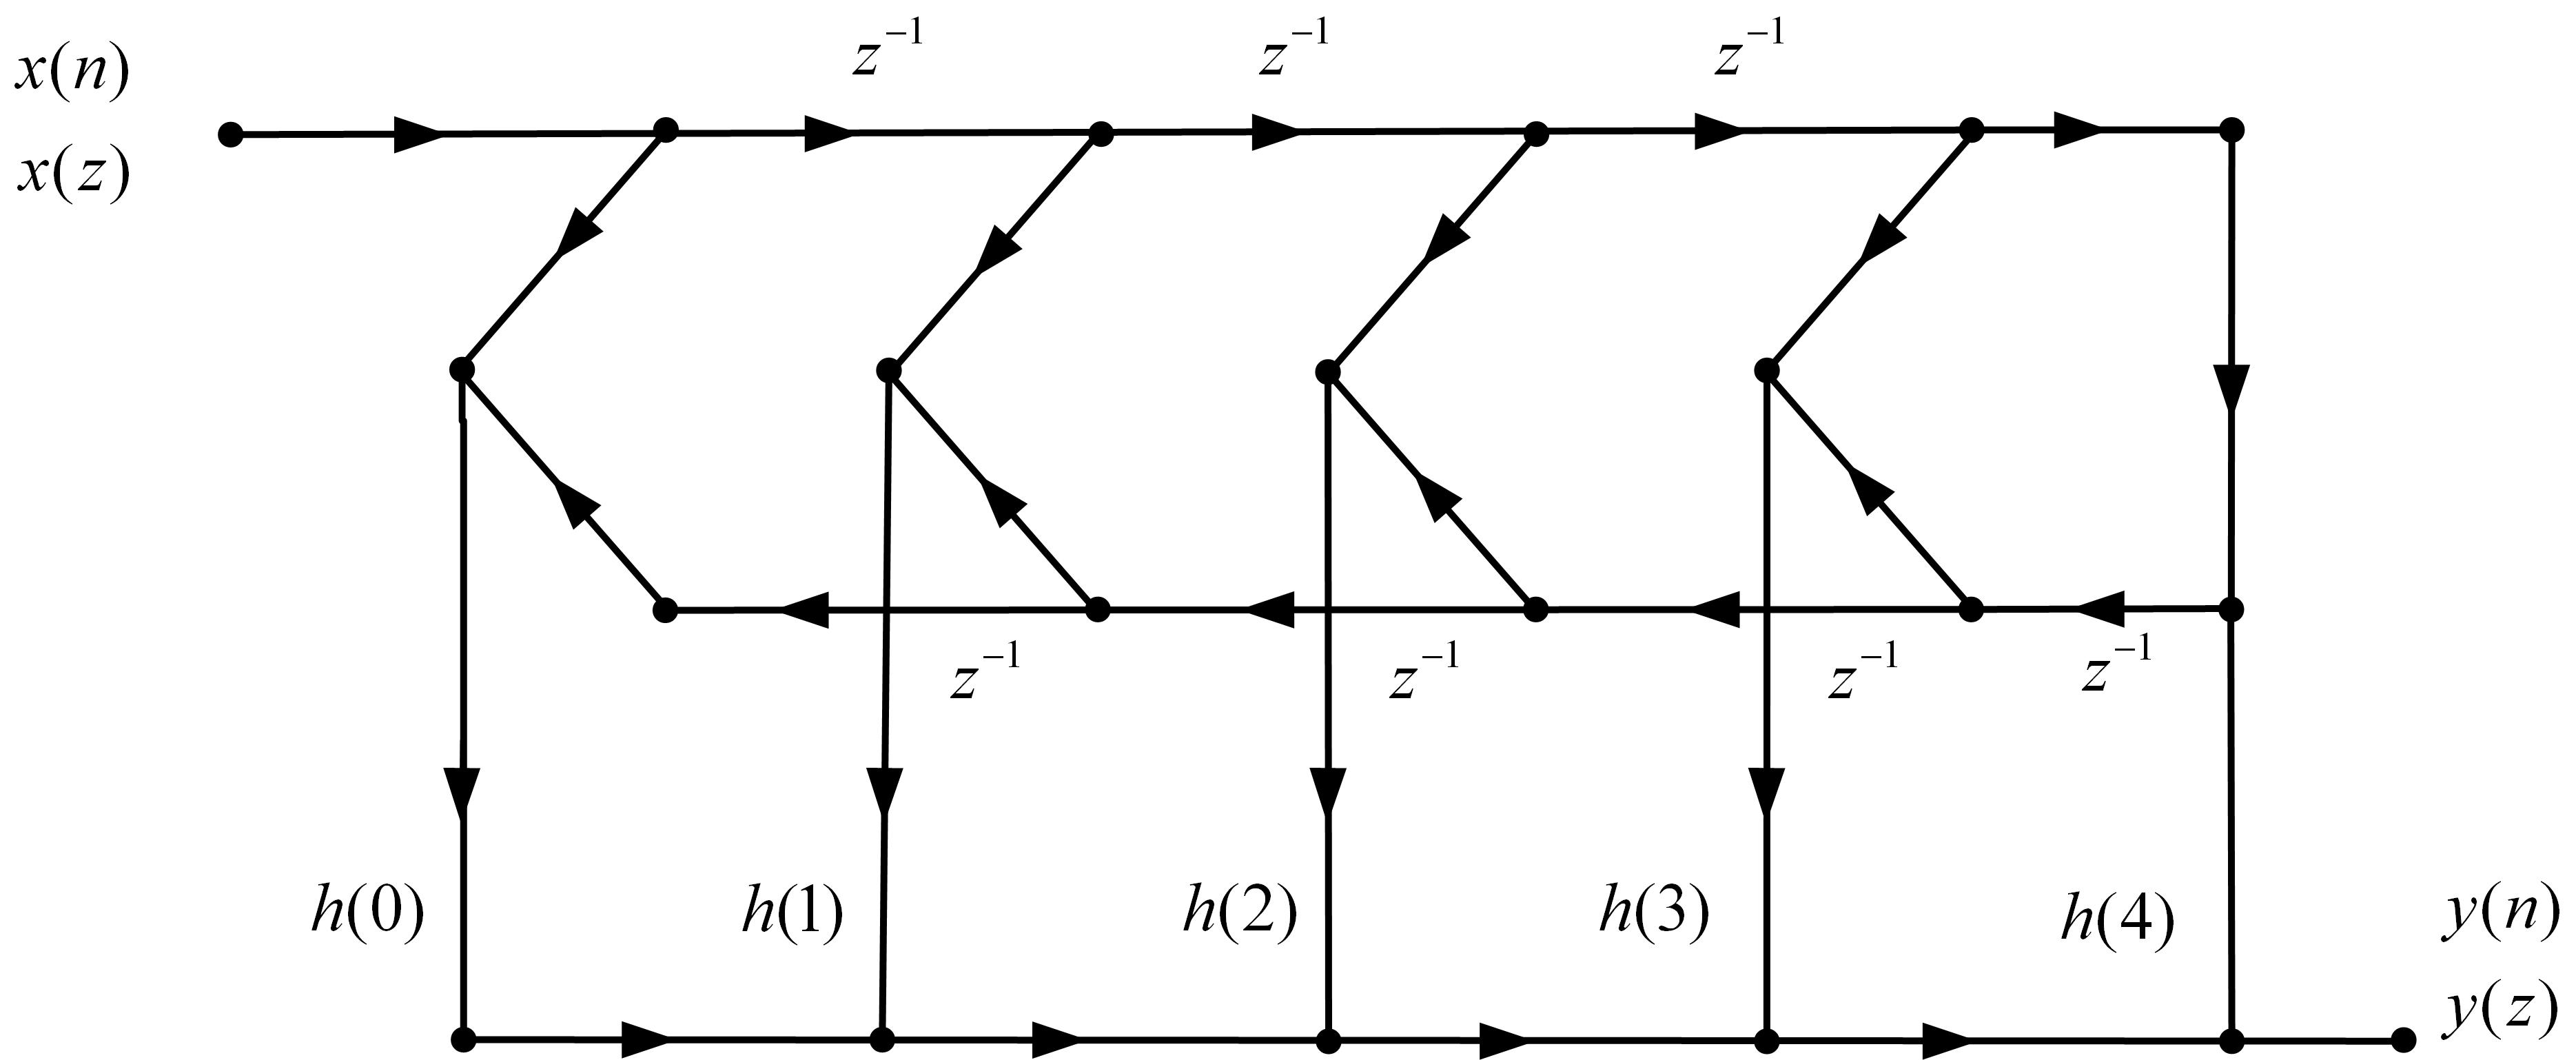
\includegraphics[width=0.85\textwidth]{jsxxxw.jpg}
%\caption{例题的第二类线性相位网络结构流图}
%\label{chp5:jibenliutu}
\end{figure}

\end{frame}
%%%%%%%%%%%%%%%%%%%%%%%%%%%%%%%%%%%%%%%%%%%%%%%%%%%%%%%%%%%%%%%%%%%%%%%%%%%%%%%%%%%%%%%%%%%%%%%%%%%%%%%%%%%%%%%%%%%%%%%%%%%%%%%%%%%%
%%%%%
%%%%%
%%%%%%%%%%%%%%%%%%%%%%%%%%%%%%%%%%%%%%%%%%%%%%%%%%%%%%%%%%%%%%%%%%%%%%%%%%%%%%%%%%%%%%%%%%%%%%%%%%%%%%%%%%%%%%%%%%%%%%%%%%%%%%%%%%%%
\begin{frame}\frametitle{(4)当N为奇数,且$h(n)= -h(N-1-n)$}%[allowframebreaks]
当N为奇数,且$h(n)= -h(N-1-n)$

    $$H(z)=\sum_{n=0}^{\frac{N}{2}-1}h(n)\left[ z^{-n}-z^{-(N-1-n)}\right]+
    h(\frac{N-1}{2})z^{-\frac{N-1}{2}}$$
\end{frame}
%%%%%%%%%%%%%%%%%%%%%%%%%%%%%%%%%%%%%%%%%%%%%%%%%%%%%%%%%%%%%%%%%%%%%%%%%%%%%%%%%%%%%%%%%%%%%%%%%%%%%%%%%%%%%%%%%%%%%%%%%%%%%%%%%%%%
%%%%%
%%%%%
%%%%%%%%%%%%%%%%%%%%%%%%%%%%%%%%%%%%%%%%%%%%%%%%%%%%%%%%%%%%%%%%%%%%%%%%%%%%%%%%%%%%%%%%%%%%%%%%%%%%%%%%%%%%%%%%%%%%%%%%%%%%%%%%%%%%
\subsubsection{线性相位结构的零点分布特性}
%%%%%%%%%%%%%%%%%%%%%%%%%%%%%%%%%%%%%%%%%%%%%%%%%%%%%%%%%%%%%%%%%%%%%%%%%%%%%%%%%%%%%%%%%%%%%%%%%%%%%%%%%%%%%%%%%%%%%%%%%%%%%%%%%%%%
%%%%%
%%%%%
%%%%%%%%%%%%%%%%%%%%%%%%%%%%%%%%%%%%%%%%%%%%%%%%%%%%%%%%%%%%%%%%%%%%%%%%%%%%%%%%%%%%%%%%%%%%%%%%%%%%%%%%%%%%%%%%%%%%%%%%%%%%%%%%%%%%
\begin{frame}[shrink]\frametitle{线性相位结构的零点分布特性}%[allowframebreaks]
%以第一类线性相位为例:设$h(n) = h(N-1-n)$
%$$\mbox{则:}\quad\quad H(z) = \sum_{n=0}^{N-1}h(n)z^{-n}\quad\quad\quad\quad\quad\quad\quad\quad\quad\quad\quad\quad$$
%令$m=N-1-n$,则:
\begin{equation*}
\begin{split}
H(z) &= \sum_{n=0}^{N-1}h(n)z^{-n} \\
     &= \sum_{m=0}^{N-1}h(N-1-m)z^{-(N-1-m)} \quad\quad(\mbox{令$m=N-1-n$}) \\
     &= \sum_{n=0}^{N-1}h(N-1-n)z^{-[(N-1)-n]} \quad\quad(\mbox{将m换为n})\\
     &= \sum_{n=0}^{N-1}h(n)z^{-(N-1)}\cdot z^{n}\quad\quad\quad\quad\quad  ( h(n) = h(N-1-n)\quad)\\
%     &= \left[\sum_{n=0}^{N-1}h(n)(z^{-1})^{-n}\right]z^{-(N-1)}\\
%     &= H(z^{-1})\cdot z^{-(N-1)}\\
\end{split}
\end{equation*}
%$$\mbox{即:}\quad\quad H(z) = z^{-(N-1)}\cdot H(z^{-1})$$
\end{frame}
%%%%%%%%%%%%%%%%%%%%%%%%%%%%%%%%%%%%%%%%%%%%%%%%%%%%%%%%%%%%%%%%%%%%%%%%%%%%%%%%%%%%%%%%%%%%%%%%%%%%%%%%%%%%%%%%%%%%%%%%%%%%%%%%%%%%
%%%%%
%%%%%
%%%%%%%%%%%%%%%%%%%%%%%%%%%%%%%%%%%%%%%%%%%%%%%%%%%%%%%%%%%%%%%%%%%%%%%%%%%%%%%%%%%%%%%%%%%%%%%%%%%%%%%%%%%%%%%%%%%%%%%%%%%%%%%%%%%%
\begin{frame}\frametitle{线性相位结构的零点分布特性}%[allowframebreaks]
以第一类线性相位为例:设$h(n) = h(N-1-n)$
%$$\mbox{则:}\quad\quad H(z) = \sum_{n=0}^{N-1}h(n)z^{-n}\quad\quad\quad\quad\quad\quad\quad\quad\quad\quad\quad\quad$$
%令$m=N-1-n$,则:
\begin{equation*}
\begin{split}
H(z) &= \sum_{n=0}^{N-1}h(n)z^{-n} \\
%     &= \sum_{m=0}^{N-1}h(N-1-m)z^{-(N-1-m)} \quad\quad(\mbox{令$m=N-1-n$}) \\
%     &= \sum_{n=0}^{N-1}h(N-1-n)z^{-[(N-1)-n]} \quad\quad(\mbox{将m换为n})\\
%     &= \sum_{n=0}^{N-1}h(n)z^{-(N-1)}\cdot z^{n}\quad\quad\quad\quad\quad  ( h(n) = h(N-1-n)\quad)\\
     &= \left[\sum_{n=0}^{N-1}h(n)(z^{-1})^{-n}\right]z^{-(N-1)}\\
     &= H(z^{-1})\cdot z^{-(N-1)}\\
\end{split}
\end{equation*}
$$\mbox{即:}\quad\quad H(z) = z^{-(N-1)}\cdot H(z^{-1})$$

\end{frame}
%%%%%
%%%%%
%%%%%%%%%%%%%%%%%%%%%%%%%%%%%%%%%%%%%%%%%%%%%%%%%%%%%%%%%%%%%%%%%%%%%%%%%%%%%%%%%%%%%%%%%%%%%%%%%%%%%%%%%%%%%%%%%%%%%%%%%%%%%%%%%%%%
\begin{frame}[shrink]\frametitle{讨论}%[allowframebreaks]
%\textbf{讨论}]
\begin{enumerate}
  \item [(1)] 对于线性相位结构,其零点关于倒数成对出现。
\end{enumerate}
%\item
设$z=z_0$是$H(z)$的任一零点,显然有$H(z_0)=0$
又,
$$H(z) = z^{-(N-1)}\cdot H(z^{-1})$$
$$\therefore\quad\quad H(z_0^{-1})=0$$
$\therefore,\quad\quad z_0^{-1}$也是$H(z)$的零点。

对于线性相位结构,其零点关于倒数成对出现。
\end{frame}


\begin{frame}[shrink]\frametitle{讨论}%[allowframebreaks]
%\item
\begin{enumerate}
  \item [(2)] 对于线性相位结构,假设$h(n)$是实数,则其零点一定是共轭成对出现。
\end{enumerate}
%又假设$h(n)$是实数,则其零点一定是共轭成对出现。

%如$H(z_0)=0$,则:
%$$H(z)   = \sum_{n=-\infty}^{\infty}h(n)z^{-n}$$
$$H(z^{*}) = \sum_{n=-\infty}^{\infty}h(n)(z^{*})^{-n}
= \underbrace{ \left[\sum_{n=-\infty}^{\infty}h(n)z^{-n}\right]^*}_{\mbox{$h(n)$是实数}}
= \left[H(z)\right]^{*}$$
如$H(z_0)=0$,则:
$$H(z_0^*) = 0$$
\end{frame}
%%%%%%%%%%%%%%%%%%%%%%%%%%%%%%%%%%%%%%%%%%%%%%%%%%%%%%%%%%%%%%%%%%%%%%%%%%%%%%%%%%%%%%%%%%%%%%%%%%%%%%%%%%%%%%%%%%%%%%%%%%%%%%%%%%%%
%%%%%
%%%%%
%%%%%%%%%%%%%%%%%%%%%%%%%%%%%%%%%%%%%%%%%%%%%%%%%%%%%%%%%%%%%%%%%%%%%%%%%%%%%%%%%%%%%%%%%%%%%%%%%%%%%%%%%%%%%%%%%%%%%%%%%%%%%%%%%%%%
\begin{frame}[shrink]\frametitle{结论}%[allowframebreaks]
对于实$h(n)$,线性相位结构数字滤波器的零点以
$$z_0,\quad\frac{1}{z_0},\quad z_0^*,\quad\frac{1}{z_0^*}$$
成组成对的形式出现,有一个是零点,其余的都是零点。
%\begin{figure}[h]
%\centering
%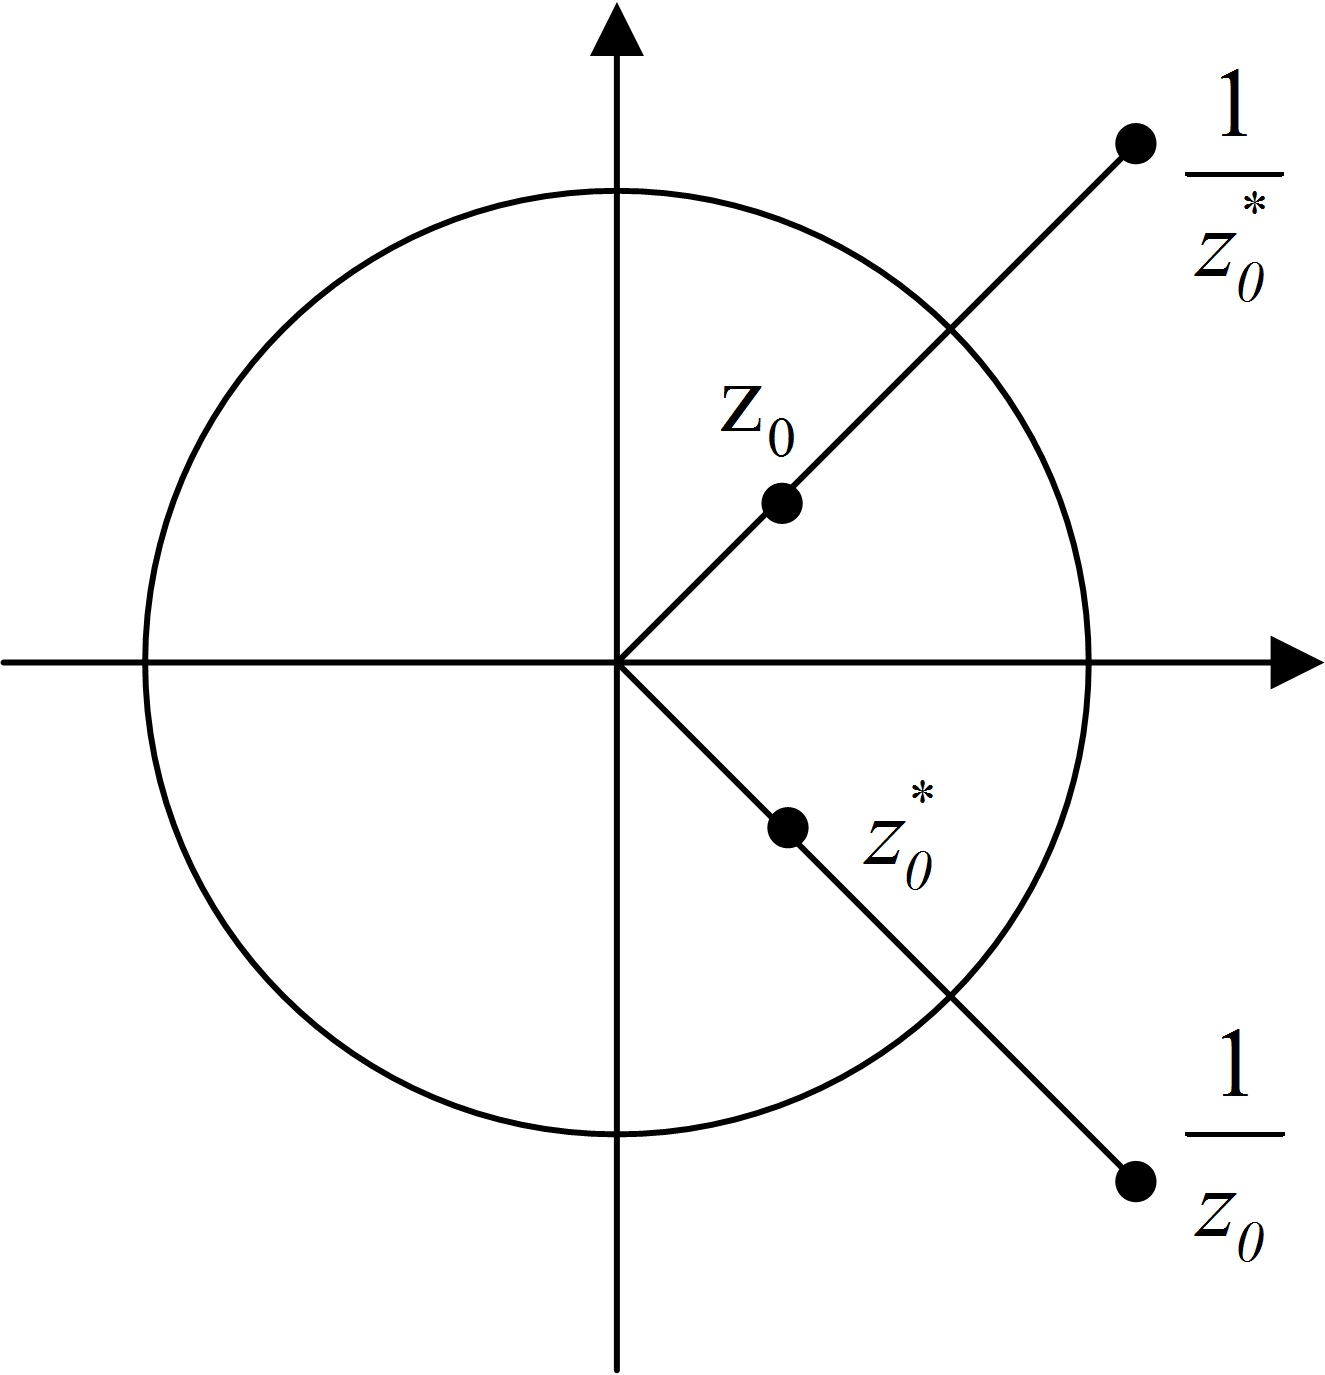
\includegraphics[width=0.35\textwidth]{xxxwldsyt.jpg}
%%\caption{线性相位结构的零点分布图}
%%\label{}
%\end{figure}
\end{frame}
%%%%%%%%%%%%%%%%%%%%%%%%%%%%%%%%%%%%%%%%%%%%%%%%%%%%%%%%%%%%%%%%%%%%%%%%%%%%%%%%%%%%%%%%%%%%%%%%%%%%%%%%%%%%%%%%%%%%%%%%%%%%%%%%%%%%
%%%%%
%%%%%
%%%%%%%%%%%%%%%%%%%%%%%%%%%%%%%%%%%%%%%%%%%%%%%%%%%%%%%%%%%%%%%%%%%%%%%%%%%%%%%%%%%%%%%%%%%%%%%%%%%%%%%%%%%%%%%%%%%%%%%%%%%%%%%%%%%%
\begin{frame}[shrink]\frametitle{零点分布的特点}%[allowframebreaks]
设$z_0= a+bi$,则
\begin{enumerate}
\item
$z_0^* = a-bi,\quad$与$z_0$关于实轴对称。
\item 有:
$$\frac{1}{z_0} = \frac{1}{a+bi} = \frac{1}{a^2+b^2}(a-bi)=
\frac{z_0^*}{a^2+b^2}$$
$\frac{1}{z_0}$与$z_0^*$同向,如$z_0^*$在单位圆内,则$\frac{1}{z_0}$在
单位圆内外。
\item 又有:
$$\frac{1}{z_0^*} = \frac{1}{a-bi} = \frac{a+bi}{a^2+b^2}
= \frac{z_0}{a^2+b^2}$$
所以,与$\frac{1}{z_0^*}$与$z_0$同向,在单位圆外。
\end{enumerate}
\end{frame}
%%%%%%%%%%%%%%%%%%%%%%%%%%%%%%%%%%%%%%%%%%%%%%%%%%%%%%%%%%%%%%%%%%%%%%%%%%%%%%%%%%%%%%%%%%%%%%%%%%%%%%%%%%%%%%%%%%%%%%%%%%%%%%%%%%%%
%%%%%
%%%%%
%%%%%%%%%%%%%%%%%%%%%%%%%%%%%%%%%%%%%%%%%%%%%%%%%%%%%%%%%%%%%%%%%%%%%%%%%%%%%%%%%%%%%%%%%%%%%%%%%%%%%%%%%%%%%%%%%%%%%%%%%%%%%%%%%%%%
\begin{frame}\frametitle{线性相位结构的零点分布图}%[allowframebreaks]
\begin{figure}[h]
\centering
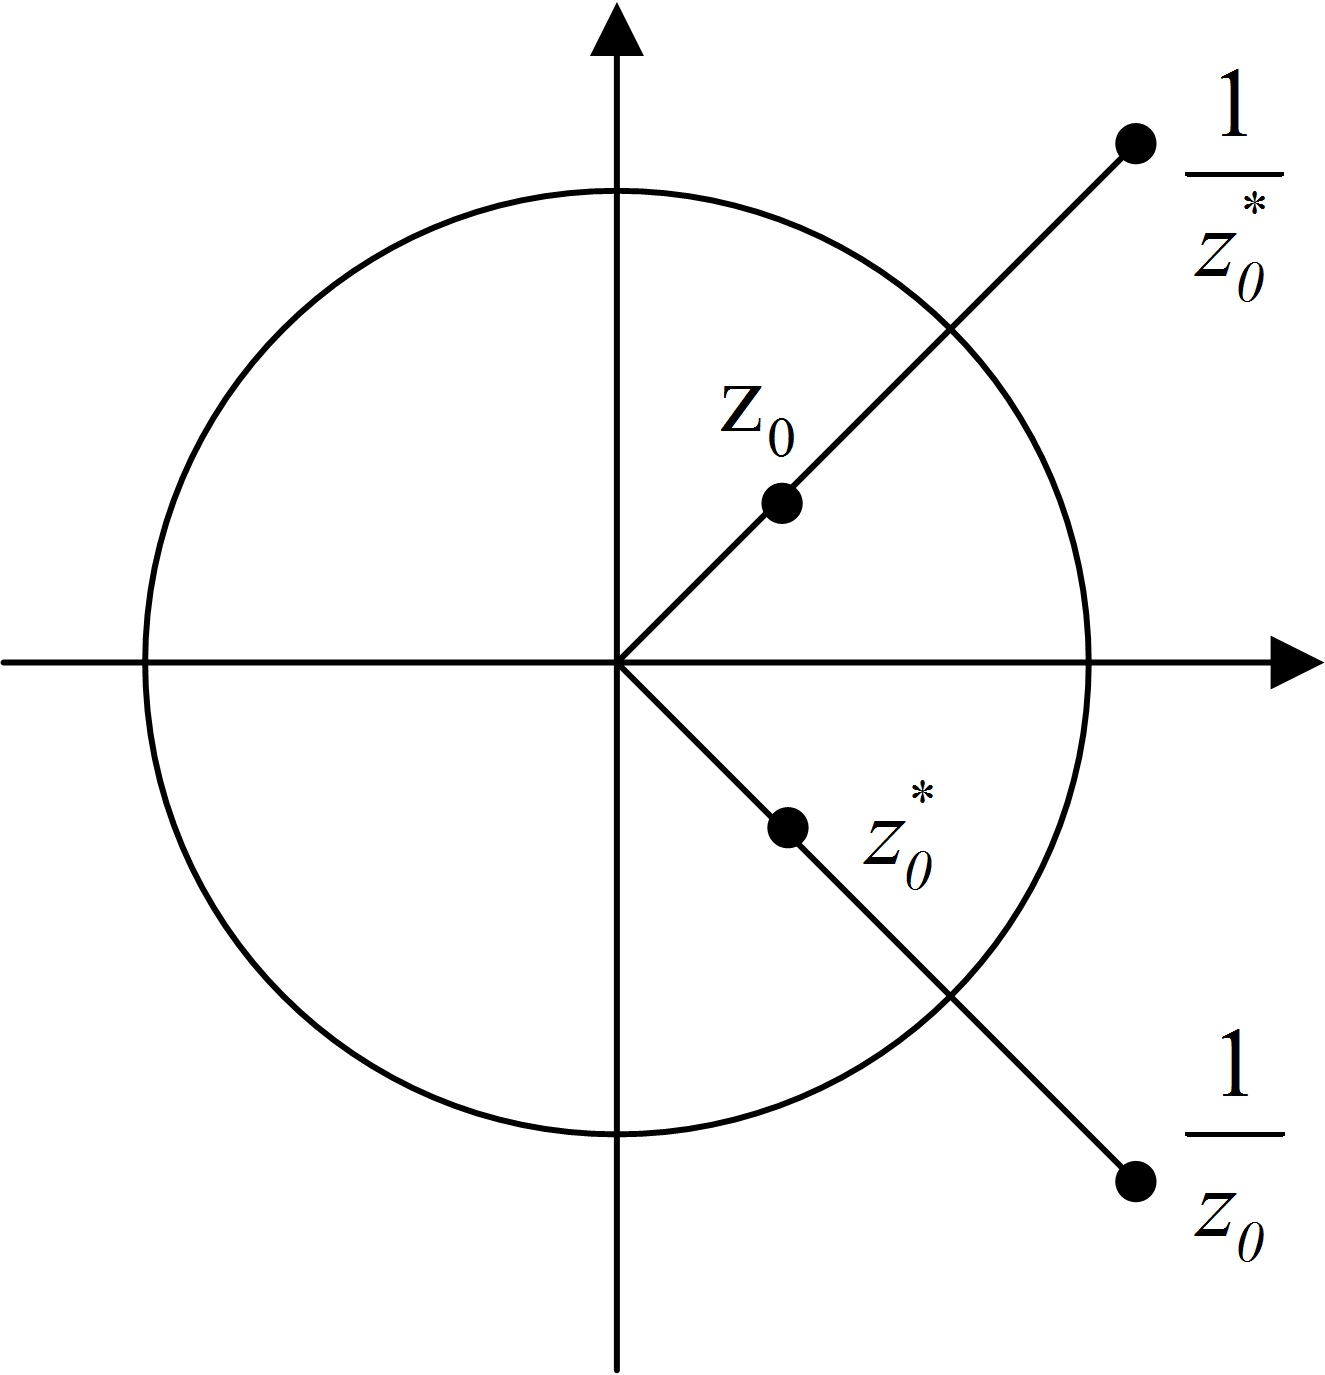
\includegraphics[width=0.6\textwidth]{xxxwldsyt.jpg}
%\caption{线性相位结构的零点分布图}
%\label{}
\end{figure}
\end{frame}
%%%%%%%%%%%%%%%%%%%%%%%%%%%%%%%%%%%%%%%%%%%%%%%%%%%%%%%%%%%%%%%%%%%%%%%%%%%%%%%%%%%%%%%%%%%%%%%%%%%%%%%%%%%%%%%%%%%%%%%%%%%%%%%%%%%%
%%%%%
%%%%%
%%%%%%%%%%%%%%%%%%%%%%%%%%%%%%%%%%%%%%%%%%%%%%%%%%%%%%%%%%%%%%%%%%%%%%%%%%%%%%%%%%%%%%%%%%%%%%%%%%%%%%%%%%%%%%%%%%%%%%%%%%%%%%%%%%%%
\begin{frame}\frametitle{进一步讨论}%[allowframebreaks]
进一步讨论
\begin{enumerate}
\item 一般情况下,4个零点的位置均不同;
\item 如$z_0$为实数,且$z_0$在横坐标上,只有两个零点;
\item 如$z_0$为虚数,且在单位圆上,只有2个零点;
\item 如$z_0$为实数,且在单位圆上,只有1个零点;
\end{enumerate}
\end{frame}
%%%%%%%%%%%%%%%%%%%%%%%%%%%%%%%%%%%%%%%%%%%%%%%%%%%%%%%%%%%%%%%%%%%%%%%%%%%%%%%%%%%%%%%%%%%%%%


\end{document}

